% Options for packages loaded elsewhere
\PassOptionsToPackage{unicode}{hyperref}
\PassOptionsToPackage{hyphens}{url}
\PassOptionsToPackage{dvipsnames,svgnames,x11names}{xcolor}
%
\documentclass[
  letterpaper,
  DIV=11,
  numbers=noendperiod]{scrreprt}

\usepackage{amsmath,amssymb}
\usepackage{lmodern}
\usepackage{iftex}
\ifPDFTeX
  \usepackage[T1]{fontenc}
  \usepackage[utf8]{inputenc}
  \usepackage{textcomp} % provide euro and other symbols
\else % if luatex or xetex
  \usepackage{unicode-math}
  \defaultfontfeatures{Scale=MatchLowercase}
  \defaultfontfeatures[\rmfamily]{Ligatures=TeX,Scale=1}
\fi
% Use upquote if available, for straight quotes in verbatim environments
\IfFileExists{upquote.sty}{\usepackage{upquote}}{}
\IfFileExists{microtype.sty}{% use microtype if available
  \usepackage[]{microtype}
  \UseMicrotypeSet[protrusion]{basicmath} % disable protrusion for tt fonts
}{}
\makeatletter
\@ifundefined{KOMAClassName}{% if non-KOMA class
  \IfFileExists{parskip.sty}{%
    \usepackage{parskip}
  }{% else
    \setlength{\parindent}{0pt}
    \setlength{\parskip}{6pt plus 2pt minus 1pt}}
}{% if KOMA class
  \KOMAoptions{parskip=half}}
\makeatother
\usepackage{xcolor}
\setlength{\emergencystretch}{3em} % prevent overfull lines
\setcounter{secnumdepth}{5}
% Make \paragraph and \subparagraph free-standing
\ifx\paragraph\undefined\else
  \let\oldparagraph\paragraph
  \renewcommand{\paragraph}[1]{\oldparagraph{#1}\mbox{}}
\fi
\ifx\subparagraph\undefined\else
  \let\oldsubparagraph\subparagraph
  \renewcommand{\subparagraph}[1]{\oldsubparagraph{#1}\mbox{}}
\fi

\usepackage{color}
\usepackage{fancyvrb}
\newcommand{\VerbBar}{|}
\newcommand{\VERB}{\Verb[commandchars=\\\{\}]}
\DefineVerbatimEnvironment{Highlighting}{Verbatim}{commandchars=\\\{\}}
% Add ',fontsize=\small' for more characters per line
\usepackage{framed}
\definecolor{shadecolor}{RGB}{241,243,245}
\newenvironment{Shaded}{\begin{snugshade}}{\end{snugshade}}
\newcommand{\AlertTok}[1]{\textcolor[rgb]{0.68,0.00,0.00}{#1}}
\newcommand{\AnnotationTok}[1]{\textcolor[rgb]{0.37,0.37,0.37}{#1}}
\newcommand{\AttributeTok}[1]{\textcolor[rgb]{0.40,0.45,0.13}{#1}}
\newcommand{\BaseNTok}[1]{\textcolor[rgb]{0.68,0.00,0.00}{#1}}
\newcommand{\BuiltInTok}[1]{\textcolor[rgb]{0.00,0.23,0.31}{#1}}
\newcommand{\CharTok}[1]{\textcolor[rgb]{0.13,0.47,0.30}{#1}}
\newcommand{\CommentTok}[1]{\textcolor[rgb]{0.37,0.37,0.37}{#1}}
\newcommand{\CommentVarTok}[1]{\textcolor[rgb]{0.37,0.37,0.37}{\textit{#1}}}
\newcommand{\ConstantTok}[1]{\textcolor[rgb]{0.56,0.35,0.01}{#1}}
\newcommand{\ControlFlowTok}[1]{\textcolor[rgb]{0.00,0.23,0.31}{#1}}
\newcommand{\DataTypeTok}[1]{\textcolor[rgb]{0.68,0.00,0.00}{#1}}
\newcommand{\DecValTok}[1]{\textcolor[rgb]{0.68,0.00,0.00}{#1}}
\newcommand{\DocumentationTok}[1]{\textcolor[rgb]{0.37,0.37,0.37}{\textit{#1}}}
\newcommand{\ErrorTok}[1]{\textcolor[rgb]{0.68,0.00,0.00}{#1}}
\newcommand{\ExtensionTok}[1]{\textcolor[rgb]{0.00,0.23,0.31}{#1}}
\newcommand{\FloatTok}[1]{\textcolor[rgb]{0.68,0.00,0.00}{#1}}
\newcommand{\FunctionTok}[1]{\textcolor[rgb]{0.28,0.35,0.67}{#1}}
\newcommand{\ImportTok}[1]{\textcolor[rgb]{0.00,0.46,0.62}{#1}}
\newcommand{\InformationTok}[1]{\textcolor[rgb]{0.37,0.37,0.37}{#1}}
\newcommand{\KeywordTok}[1]{\textcolor[rgb]{0.00,0.23,0.31}{#1}}
\newcommand{\NormalTok}[1]{\textcolor[rgb]{0.00,0.23,0.31}{#1}}
\newcommand{\OperatorTok}[1]{\textcolor[rgb]{0.37,0.37,0.37}{#1}}
\newcommand{\OtherTok}[1]{\textcolor[rgb]{0.00,0.23,0.31}{#1}}
\newcommand{\PreprocessorTok}[1]{\textcolor[rgb]{0.68,0.00,0.00}{#1}}
\newcommand{\RegionMarkerTok}[1]{\textcolor[rgb]{0.00,0.23,0.31}{#1}}
\newcommand{\SpecialCharTok}[1]{\textcolor[rgb]{0.37,0.37,0.37}{#1}}
\newcommand{\SpecialStringTok}[1]{\textcolor[rgb]{0.13,0.47,0.30}{#1}}
\newcommand{\StringTok}[1]{\textcolor[rgb]{0.13,0.47,0.30}{#1}}
\newcommand{\VariableTok}[1]{\textcolor[rgb]{0.07,0.07,0.07}{#1}}
\newcommand{\VerbatimStringTok}[1]{\textcolor[rgb]{0.13,0.47,0.30}{#1}}
\newcommand{\WarningTok}[1]{\textcolor[rgb]{0.37,0.37,0.37}{\textit{#1}}}

\providecommand{\tightlist}{%
  \setlength{\itemsep}{0pt}\setlength{\parskip}{0pt}}\usepackage{longtable,booktabs,array}
\usepackage{calc} % for calculating minipage widths
% Correct order of tables after \paragraph or \subparagraph
\usepackage{etoolbox}
\makeatletter
\patchcmd\longtable{\par}{\if@noskipsec\mbox{}\fi\par}{}{}
\makeatother
% Allow footnotes in longtable head/foot
\IfFileExists{footnotehyper.sty}{\usepackage{footnotehyper}}{\usepackage{footnote}}
\makesavenoteenv{longtable}
\usepackage{graphicx}
\makeatletter
\def\maxwidth{\ifdim\Gin@nat@width>\linewidth\linewidth\else\Gin@nat@width\fi}
\def\maxheight{\ifdim\Gin@nat@height>\textheight\textheight\else\Gin@nat@height\fi}
\makeatother
% Scale images if necessary, so that they will not overflow the page
% margins by default, and it is still possible to overwrite the defaults
% using explicit options in \includegraphics[width, height, ...]{}
\setkeys{Gin}{width=\maxwidth,height=\maxheight,keepaspectratio}
% Set default figure placement to htbp
\makeatletter
\def\fps@figure{htbp}
\makeatother

\usepackage{booktabs}
\usepackage{siunitx}

  \newcolumntype{d}{S[
    input-open-uncertainty=,
    input-close-uncertainty=,
    parse-numbers = false,
    table-align-text-pre=false,
    table-align-text-post=false
  ]}
  
\usepackage{longtable}
\usepackage{array}
\usepackage{multirow}
\usepackage{wrapfig}
\usepackage{float}
\usepackage{colortbl}
\usepackage{pdflscape}
\usepackage{tabu}
\usepackage{threeparttable}
\usepackage{threeparttablex}
\usepackage[normalem]{ulem}
\usepackage{makecell}
\usepackage{xcolor}
\KOMAoption{captions}{tableheading}
\makeatletter
\makeatother
\makeatletter
\@ifpackageloaded{bookmark}{}{\usepackage{bookmark}}
\makeatother
\makeatletter
\@ifpackageloaded{caption}{}{\usepackage{caption}}
\AtBeginDocument{%
\ifdefined\contentsname
  \renewcommand*\contentsname{Table of contents}
\else
  \newcommand\contentsname{Table of contents}
\fi
\ifdefined\listfigurename
  \renewcommand*\listfigurename{List of Figures}
\else
  \newcommand\listfigurename{List of Figures}
\fi
\ifdefined\listtablename
  \renewcommand*\listtablename{List of Tables}
\else
  \newcommand\listtablename{List of Tables}
\fi
\ifdefined\figurename
  \renewcommand*\figurename{Figure}
\else
  \newcommand\figurename{Figure}
\fi
\ifdefined\tablename
  \renewcommand*\tablename{Table}
\else
  \newcommand\tablename{Table}
\fi
}
\@ifpackageloaded{float}{}{\usepackage{float}}
\floatstyle{ruled}
\@ifundefined{c@chapter}{\newfloat{codelisting}{h}{lop}}{\newfloat{codelisting}{h}{lop}[chapter]}
\floatname{codelisting}{Listing}
\newcommand*\listoflistings{\listof{codelisting}{List of Listings}}
\usepackage{amsthm}
\theoremstyle{definition}
\newtheorem{exercise}{Exercise}[chapter]
\theoremstyle{remark}
\renewcommand*{\proofname}{Proof}
\newtheorem*{remark}{Remark}
\newtheorem*{solution}{Solution}
\makeatother
\makeatletter
\@ifpackageloaded{caption}{}{\usepackage{caption}}
\@ifpackageloaded{subcaption}{}{\usepackage{subcaption}}
\makeatother
\makeatletter
\@ifpackageloaded{tcolorbox}{}{\usepackage[many]{tcolorbox}}
\makeatother
\makeatletter
\@ifundefined{shadecolor}{\definecolor{shadecolor}{rgb}{.97, .97, .97}}
\makeatother
\makeatletter
\makeatother
\ifLuaTeX
  \usepackage{selnolig}  % disable illegal ligatures
\fi
\IfFileExists{bookmark.sty}{\usepackage{bookmark}}{\usepackage{hyperref}}
\IfFileExists{xurl.sty}{\usepackage{xurl}}{} % add URL line breaks if available
\urlstyle{same} % disable monospaced font for URLs
\hypersetup{
  pdftitle={Forkurs for kvantitativ metode},
  pdfauthor={Torbjørn Skardhamar},
  colorlinks=true,
  linkcolor={blue},
  filecolor={Maroon},
  citecolor={Blue},
  urlcolor={Blue},
  pdfcreator={LaTeX via pandoc}}

\title{Forkurs for kvantitativ metode}
\usepackage{etoolbox}
\makeatletter
\providecommand{\subtitle}[1]{% add subtitle to \maketitle
  \apptocmd{\@title}{\par {\large #1 \par}}{}{}
}
\makeatother
\subtitle{Forkurs til SOS4020}
\author{Torbjørn Skardhamar}
\date{8/9/23}

\begin{document}
\maketitle
\ifdefined\Shaded\renewenvironment{Shaded}{\begin{tcolorbox}[interior hidden, borderline west={3pt}{0pt}{shadecolor}, boxrule=0pt, sharp corners, breakable, enhanced, frame hidden]}{\end{tcolorbox}}\fi

\renewcommand*\contentsname{Table of contents}
{
\hypersetup{linkcolor=}
\setcounter{tocdepth}{2}
\tableofcontents
}
\bookmarksetup{startatroot}

\hypertarget{forord}{%
\chapter*{Forord}\label{forord}}
\addcontentsline{toc}{chapter}{Forord}

\markboth{Forord}{Forord}

Dette materialet er beregnet på et forkurs for masterstudenter i
sosiologi ved universitet i Oslo som skal ta emnet
\href{https://www.uio.no/studier/emner/sv/iss/SOS4020/}{SOS4020
Kvantitative metoder}. Forkurset dekker de mest sentrale elementene fra
BA-nivået som trengs for å ta SOS4020.

Det anbefales å repetere materiale fra kurs i kvantitative metoder på
bachelornivå. Forkurset er en oppfrisker av det aller viktigste
materialet fra
\href{https://www.uio.no/studier/emner/sv/iss/SOSGEO1120/}{SOSGEO1120}.

De som lært annen statistikksoftware enn R på bachelornivå vil ha særlig
nytte av dette kurset. Har man tatt bachelorgrad annet sted enn ved UiO
kan man ha lært å bruke Stata, SPSS eller noe slikt. Da trenger du en
introduksjon til R, men hva vi skal gjøre vil være tilsvarende.

En av de store forskjellene fra SPSS og Stata er at R \textbf{ikke} har
muligheten for menybaserte analyser. Du kan altså ikke gjøre analyser
med ``pek-og-klikk''! Det bør du jo egentlig uansett ikke gjøre i annen
software heller. R er altså et programmeringsspråk, og det er viktig å
lære å skrive kode både for databehandling og analyse. I tillegg til
programmeringsspråket skal du lære å lage en hensiktsmessig
mappestruktur og lese inn datasett i R.

Datasettet som skal brukes i SOS4020 er tilgangsbegrenset så det er litt
formaliteter som må på plass først. Det skal vi gå på plass her slik at
dere har lovlig tilgang til dataene. Men gjennomgangen og eksempler i
det følgende vil basere seg på det samme datasett som brukes
gjennomgående i SOSGEO1120. Til hvert kapittel er det oppgaver. Først og
fremst skal dere kunne gjøre de samme operasjonene på egen datamaskin.
Dernest skal dere bruke NorLAG til å gjøre noe mer selvstendige analyser
med de samme teknikkene.

Dette heftet inneholder også bittelitt mer informasjon enn du trenger
(f.eks. appendiks), men som du kan ha bruk for hvis du skal gjøre mer
selvstendige analyser senere.

\hypertarget{muxe5lsettinger-for-forkurset}{%
\section*{Målsettinger for
forkurset}\label{muxe5lsettinger-for-forkurset}}
\addcontentsline{toc}{section}{Målsettinger for forkurset}

\markright{Målsettinger for forkurset}

Overordnet sett skal du denne uken bli kjent med hvordan du bruker R til
dataanalyse og repetert grunnleggende statistikk. Du jobber i eget
tempo. Bruk tid på det som er krevende og hopp gjerne over deler du
synes er enkelt. Så ber du om hjelp når du trenger det. Lærere er
tilstede to timer på starten av dagen, og stikker antakeligvis innom en
tur på slutten av dagen også. Bruk oss!

Husk at det er ingen eksamen og krav på et slikt forkurs, så det er opp
til deg å bruke tiden som er best for deg. Det blir vesentlig enklere å
ta kurset SOS4020 hvis du har det grunnleggende rimelig på plass først.

Her er en tentativ plan for hva du bør gjennom disse dagene:

\textbf{Dag 1}

\begin{itemize}
\tightlist
\item
  R og Rstudio er installert riktig på egen maskin.
\item
  Mappestruktur og opprettet Rstudio-project.
\item
  Tilgang til NorLAG og avtale for bruk, regler for datalagring
\item
  Innlesning av data i .rds og .dta format
\item
  Startet med praktisk grafikk
\end{itemize}

\textbf{Dag 2}

\begin{itemize}
\tightlist
\item
  Grafikk og tabeller.
\item
  Grunnleggende om objekter og dplyr-verb, inkludert pipe-operator.
\end{itemize}

\textbf{Dag 3}

\begin{itemize}
\tightlist
\item
  Grunnleggende regresjon.
\item
  Sannsynlighet: standardfeil, p-verdier og konfidensintervall
\end{itemize}

\textbf{Dag 4}

\begin{itemize}
\tightlist
\item
  Sannsynlighet (forts.)
\item
  \emph{Anvende} standardfeil, p-verdier og konfidensintervall sammen
  med teknikker gjennomgått første dag (tabeller og regresjon)
\end{itemize}

\part{Del 1: Kom igang}

\hypertarget{oppgaver}{%
\chapter{Oppgaver}\label{oppgaver}}

Man lærer aller best ved å jobbe selv og få hjelp underveis. Dette
forkurset er derfor lagt opp til at du skal jobbe på egenhånd, og det
blir ingen forelesninger. Dette heftet går gjennom hvordan man gjør en
rekke praktiske oppgaver med bruk av softwaren R, og dekker dermed
grafikk, deskriptiv statistikk, regresjonsmodeller, og statistisk
tolkning. Tilhørende er grunnleggende databehandling som jo også trengs.

\hypertarget{gjuxf8r-det-puxe5-egen-datamaskin}{%
\section{Gjør det på egen
datamaskin}\label{gjuxf8r-det-puxe5-egen-datamaskin}}

Heftet bruker gjennomgående et enkelt datasett \emph{abu89} og viser
R-koden illustrerer dermed hvordan ting gjøres. Det første du skal gjøre
er dermed å gjøre det samme på egen datamaskin og sjekke at du får samme
resultat. Dette kan gjøres som en enkel ``klipp-og-lim'' som du neppe
lærer så veldig mye av hvis du ikke tenker litt samtidig, men du får i
hvert fall sjekket at koden fungerer. For hver operasjon bør du gjøre
noen endringer i koden og se hva som skjer. I kapittelet om grafikk kan
du f.eks. eksperimentere med å bytte om på variable, endre farger og
annet. Slik får du en bedre forståelse av hva de ulike funksjonene og
argumentene betyr. En god måte å finne ut av hvordan ting fungerer er å
gjøre endringer og se hva som skjer.

\hypertarget{gjuxf8r-tilsvarende-med-datasettet-norlag}{%
\section{Gjør tilsvarende med datasettet
NorLAG}\label{gjuxf8r-tilsvarende-med-datasettet-norlag}}

Jo mer du tenker aktivt selv, jo mer lærer du. Bruk et annet datasett og
gjør tilsvarende operasjoner som er vist med \emph{abu89}. Dere får
tilgang til et stort datasett fra undersøkelsen NorLAG og kan da
undersøke mange muligheter.

Du kan gjerne prøve å replikere noen tidligere studier som du finner i
\href{https://norlag.nsd.no/publications}{denne
publikasjonslista}.\^{}(OBS! Å replikere andres studier nøyaktig er
langt mer krevende enn man skulle tro. Normalt trenger du at forfatter
deler originalt script, men det er ikke alltid lett tilgjengelig,
skrevet i et annet programmeringsspråk, inkluderer langt mer avanserte
teknikker enn du har lært om, eller bare er generelt uryddig. Så ikke
sett det som ambisjon, men få heller inspirasjon til å finne et tema som
er litt interessant og søk opp aktuelle variable.) Variabelliste med
dokumentasjon finner du filen ``Kodebok.html'' når du har fått tilgang
til delt mappe .

\hypertarget{bruk-helt-andre-datasett}{%
\section{Bruk helt andre datasett}\label{bruk-helt-andre-datasett}}

Det er en god del innebygde datasett i R og i ulike R-pakker. Du kan få
en oversikt over tilgjengelig datasett ved funksjonen \texttt{data()}
som lister opp de dataene som er tilgjengelig i de pakkene du har lastet
for øyeblikket.

\begin{itemize}
\tightlist
\item
  causaldata: en pakke med diverse datasett brukt i lærebøker for
  kausalanalyse. Tilgang: \texttt{install.packages(causaldata)}. For en
  oversikt, se pakkes
  \href{https://cran.r-project.org/web/packages/causaldata/causaldata.pdf}{dokumentasjon}.
\item
  gapminder: en pakke med utdrag av
  \href{https://www.gapminder.org/data/}{Gapminder-data} med ulike lands
  levealder, befolkningsstørrelse og brutto nasjonalprodukt over mange
  år. Tilgang: \texttt{install.packages(gapminder)}
\end{itemize}

Når en pakke, f.eks. gapminder, er lastet har du automatisk tilgang til
dataene ved å bruke navnet på datasettet i en funksjon som følger:

\begin{Shaded}
\begin{Highlighting}[]
\FunctionTok{library}\NormalTok{(gapminder)}
\FunctionTok{summary}\NormalTok{(gapminder)}
\end{Highlighting}
\end{Shaded}

\begin{verbatim}
        country        continent        year         lifeExp     
 Afghanistan:  12   Africa  :624   Min.   :1952   Min.   :23.60  
 Albania    :  12   Americas:300   1st Qu.:1966   1st Qu.:48.20  
 Algeria    :  12   Asia    :396   Median :1980   Median :60.71  
 Angola     :  12   Europe  :360   Mean   :1980   Mean   :59.47  
 Argentina  :  12   Oceania : 24   3rd Qu.:1993   3rd Qu.:70.85  
 Australia  :  12                  Max.   :2007   Max.   :82.60  
 (Other)    :1632                                                
      pop              gdpPercap       
 Min.   :6.001e+04   Min.   :   241.2  
 1st Qu.:2.794e+06   1st Qu.:  1202.1  
 Median :7.024e+06   Median :  3531.8  
 Mean   :2.960e+07   Mean   :  7215.3  
 3rd Qu.:1.959e+07   3rd Qu.:  9325.5  
 Max.   :1.319e+09   Max.   :113523.1  
                                       
\end{verbatim}

\hypertarget{installere-r-og-rstudio}{%
\chapter{Installere R og Rstudio}\label{installere-r-og-rstudio}}

Vi forutsetter grunnleggende kunnskap til bruk av datamaskiner, og hvis
du oppdager at det er tekniske ting du ikke får til forutsetter vi at du
lærer deg det. Det går også an å spørres seminarleder om hjelp, men gjør
det unna tidlig i semesteret. Her er noe av det vi forutsetter:

Laste ned og installere programmer på datamaskinen Lage mapper og
mappestruktur på lokal maskin, og holde oversikt over filer på din
datamaskin Laste ned en fil direkte til en mappe uten å åpne, herunder
lokalisere download-mappen

OBS! Det er mange csv-filer tilknyttet oppgaver i læreboken. Sørg for å
laste ned filene uten at de først åpnes i Excel med en gang. Grunnen er
at selv om det stort sett går greit, er Excel tilbøyelig til å tenke
litt mye selv og kan finne på å forandre datasettet. (Hvis dette skjer
på eksamen er du i trøbbel, så unngå det!).

\hypertarget{installasjon}{%
\section{Installasjon}\label{installasjon}}

Installer nyeste versjon av R herfra: https://cran.uib.no/ Du trenger
det som heter «base» når man installerer for første gang. Hvis du har R
installert på maskinen din fra før, sørg for at du har siste versjon
installert. Siste versjon er 4.1.2. Versjon etter 4.0 bør gå bra, men
tidligere versjoner vil kunne gi problemer. Installer nyeste versjon av
RStudio (gratisversjon) herfra:
https://rstudio.com/products/rstudio/download/ Viktig: du må installere
R før du installerer Rstudio for Rstudio finner R på din datamaskin og
vil gi feilmelding hvis den ikke finner R. Hvis du har en eldre
datamaskin og du får feilmelding ved installasjon av RStudio kan du
vurdere å installere forrige versjon av Rstudio herfra:
https://www.rstudio.com/products/rstudio/older-versions/

R og Rstudio er to programmer er integrert i hverandre og du åpner
heretter R ved å åpne RStudio. Merk: R er navnet på
programmeringsspråket og programmet som gjør selve utregningene. Det
kjører fra en kommandolinje og er ikke veldig brukervennlig alene.
RStudio er et ``integrated development environment'' (IDE) til R. Det
integrerer R med en konsoll, grafikk-vindu og en del andre nyttige ting.
Det gjør det lettere å bruke R.

Det finnes også andre IDE for R, men vi skal bruke RStudio gjennomgående
på dette kurset. (RStudio inneholder også masse annen funksjonalitet vi
ikke trenger til dette kurset).

\hypertarget{spesielt-om-windows-maskiner-installer-rtools}{%
\subsection{Spesielt om Windows-maskiner: installer
Rtools}\label{spesielt-om-windows-maskiner-installer-rtools}}

Hvis du jobber på en Windows-maskin må du også installere Rtools herfra:
https://cran.r-project.org/bin/windows/Rtools/

\hypertarget{spesielt-om-mac-maskiner}{%
\subsection{Spesielt om Mac-maskiner}\label{spesielt-om-mac-maskiner}}

R skal normalt installere på Mac uten problemer. Noen har fått beskjed
om at de også trenger å installere XQuartz eller Xcode. I så fall
installerer du de også. Se mer informasjon her:
https://cran.r-project.org/bin/macosx/tools/

\hypertarget{spesielt-om-linux-maskiner}{%
\subsection{Spesielt om
Linux-maskiner}\label{spesielt-om-linux-maskiner}}

Har du Linux vet du antakelig hva du driver med. Siste versjon av R og
Rstudio kan antakeligvis installeres fra distroens repository.

\hypertarget{spesielt-om-chromebook}{%
\subsection{Spesielt om Chromebook}\label{spesielt-om-chromebook}}

Chromebook kjører et annet operativsystem og R vil ikke uten videre
fungere. Derimot kan man på de fleste slike maskiner åpne opp for å
kjøre Linux og da kan man installere linux-versjon av R og Rstudio.
https://blog.sellorm.com/2018/12/20/installing-r-and-rstudio-on-a-chromebook/
Eller se nedenfor hvordan du kan kjøre R i skyen.

\hypertarget{oppsett-og-forberedelser}{%
\section{Oppsett og forberedelser}\label{oppsett-og-forberedelser}}

Dette oppsettet gjelder både hvis du har en lokal installasjon og for
skyløsninger. Utseendet spiller ingen rolle, og R kan også fungere uten
å opprette «projects» som beskrevet her. Men det er lettere å bruke og
du har bedre orden hvis du gjør dette.

\hypertarget{utseende-i-rstudio}{%
\subsection{Utseende i Rstudio}\label{utseende-i-rstudio}}

Endre gjerne på oppsettet i RStudio ved å gå til Tools og deretter
Global options, så Pane Layout.

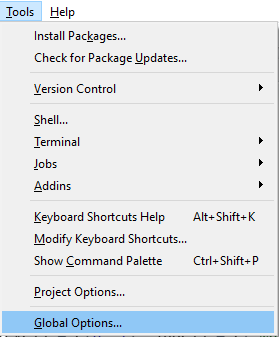
\includegraphics{./images/oppsett1.png}

Det spiller ingen rolle for funksjonaliteten hvor du har hvilken fane,
men her er et forslag.

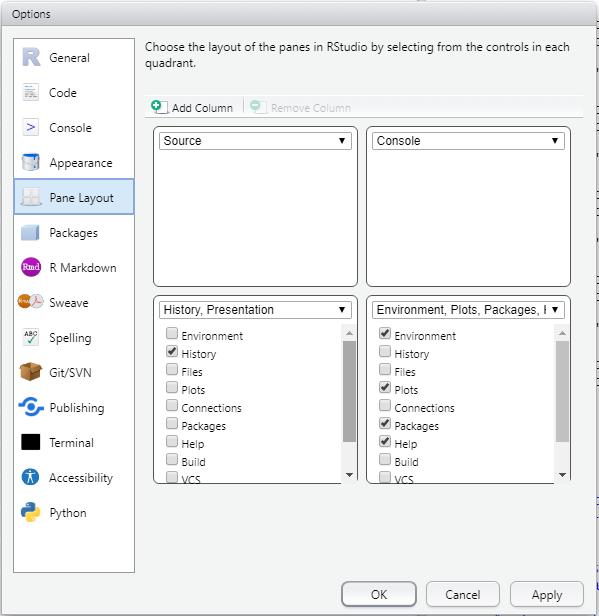
\includegraphics{./images/oppsett2.png}

Dette kan også endres senere og har altså bare med hvordan Rstudio ser
ut.

\hypertarget{rstudio-projects}{%
\section{Rstudio projects}\label{rstudio-projects}}

Når du åpner Rstudio skal du alltid åpne som «project» (se video med
instruksjon og i R4DS). Arbeidsområdet er da definert og du kan åpne
data ved å bruke relative filbaner, dvs. at du oppgir hvor dataene
ligger med utgangspunkt i prosjektmappen. Se kursvideo og instruksjoner
i R4DS og gjør følgende:

Opprettet mappestruktur med SOSGEO1120 som øverste nivå og egne
undermapper for data, script, og output.

\hypertarget{uxe5pne-rstudio-og-opprett-et-.rproject}{%
\section{Åpne RStudio og opprett et
.Rproject}\label{uxe5pne-rstudio-og-opprett-et-.rproject}}

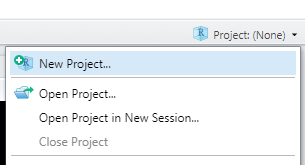
\includegraphics{./images/proj2.png}

Bruk kommandoen getwd() og se at du har riktig filbane til
arbeidsområdet. Hvis du ikke er sikker på hva det betyr, må du spørre
noen eller finne det ut på annen måte!

Det første dere må gjøre er å sørge for å ha orden i datasett, script og
annet på din egen datamaskin. Å f.eks. lagre alle filer på skrivebordet
bør du aldri gjøre, og særlig ikke i dette kurset eller når man jobber
med større prosjekter og datasett. For dette kurset skal du ha en
mappestruktur med en hovedmappe for SOSGEO1120 og tilhørende
undermapper. Det spiller ingen rolle hvor på datamaskinen du legger
disse mappene, men du må vite hvor det er. Lag første en mappe som heter
SOSGEO1120, og innunder denne mappen lager du tre andre mapper med
navnene data, output og script. Du kan ha andre mapper i tillegg ved
behov. Det kan se slik ut:

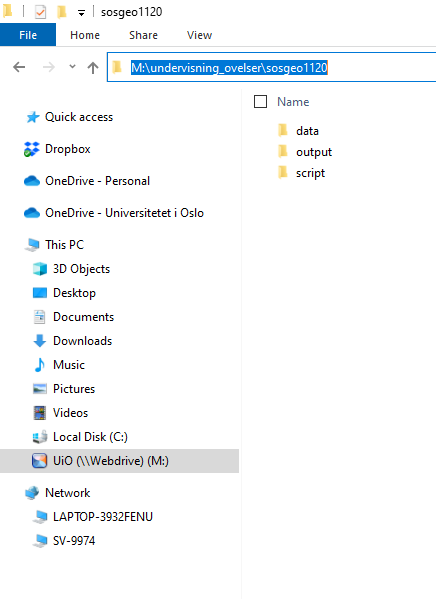
\includegraphics{./images/proj1.png}

Du skal opprette et Rstudio-prosjekt for hele kurset. Dette er beskrevet
nærmere i R4DS i kapittel 6. Når du har åpnet RStudio skal du aller
først klikke New Project.

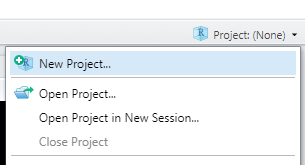
\includegraphics{./images/proj2.png}

Deretter klikker du du «Existing Directory»

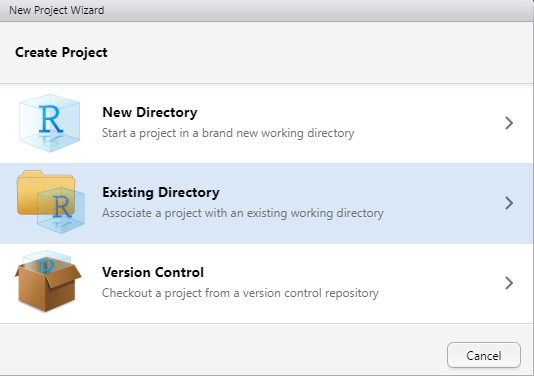
\includegraphics{./images/proj3.png}

Klikk «Browse» og bla deg så frem til mappen du har laget for
SOSGEO1120.

RStudio-prosjektet ligger så i den mappen du har valgt. I filutforsker
på datamaskinen vil nå disse to filene dukke opp:

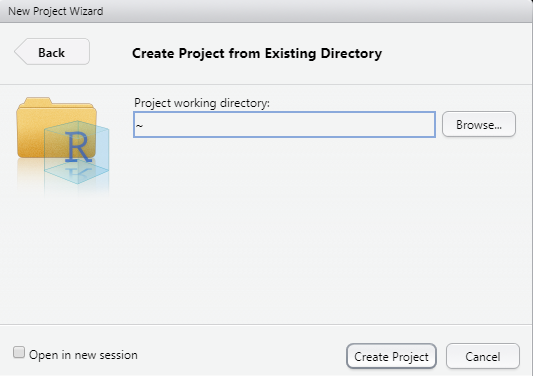
\includegraphics{./images/proj4.png}

For å starte R videre i dette kurset skal du dobbeltklikke det første
ikonet, så vil R åpne seg med riktig arbeidsområde. Mappen .Rproj.user
skal du ikke røre. I RStudio vil du se at prosjektet er åpnet ved at det
i øvre høyre hjørne er dette ikonet:

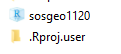
\includegraphics{./images/proj5.png}

En stor fordel med å bruke projects er at du kan flytte hele mappen til
et annet sted, eller til en annen datamaskin og alt vil fungere akkurat
som før. Hvis du bruker en skytjeneste (OneDrive, Dropbox etc) vil du
kunne åpne Rstudio projects på samme måte fra flere maskiner.

\hypertarget{en-veldig-kjapp-intro-til-r}{%
\chapter{En veldig kjapp intro til
R}\label{en-veldig-kjapp-intro-til-r}}

Før vi setter igang trengs det en kort introduksjon til noe
grunnleggende om hvordan R fungerer. Så lærer man mer underveis, og et
senere kapittel går grundigere inn i omkoding av variable.

\hypertarget{objektorientert}{%
\section{Objektorientert}\label{objektorientert}}

I de innledende kapitlene ble det vist hvordan man leser inn data i R og
dataene ble lagt i et ``objekt''. R er bygd opp rundt å bruke slike
objekter i den forstand at alt man jobber med (typisk: datasett) ligger
i objekter.

Du kan tenke på objekter som en boks som det står et navn på. Ofte er
det bare et datasett oppi boksen, men det kan også være flere ting. Det
finnes derfor \emph{flere typer objekter}. Vi skal primært jobbe med
datasett, og slike objekter er av typen ``data.frame''. De kan også være
av typen ``tibble'', men det er for alle praktiske formål på dette
nivået akkurat det samme som ``data.frame''. Men objekter kan også
inneholde resultater fra analyser, som f.eks. grafikk, tabeller eller
regresjonsresultater. Man kan også legge enkelttall, vektorer og
tekststrenger i objekter.

Noen ganger vil et objekt inneholde flere forskjellige ting. Et eksempel
er resultat fra regresjonsmodeller som både vil inneholde koeffisienter,
standardfeil, residualer, en del statistikker, men også selve
datasettet. Men for å se på output er det funksjoner som trekker ut
akkurat det vi trenger, så du trenger sjelden forholde deg til hvordan
et slikt objekt er bygd opp. Men du kan tenke på det som en
velorganisert boks med masse mindre rom oppi.

Men poenget er: Alt du jobber med i R er objekter. Alle objekter har et
navn som du velger selv. Du kan legge hva som helst i et objekt. Du kan
ikke ha to objekter med samme navn, og hvis du lager et objekt med et
navn som eksisterer fra før overskriver du det gamle objektet.

\hypertarget{funksjoner}{%
\section{Funksjoner}\label{funksjoner}}

Alt man gjør i R gjøres med ``funksjoner'', og man bruker funksjonene på
objekter eller deler av objekter. Funksjonenen har et navn og etterfulgt
av en parentes slik som f.eks. \texttt{dinfunksjon(...)}. Funksjonen
starter og slutter med en parentes. Du kan tenke på funksjoner som en
liten maskin der du putter noe inn, og så kommer noe annet ut. Det du
putter inn skal står inni parentes. Det som kommer ut kan du enten legge
i et eget objekt eller la det skrives til output-vinduet.

Det du legger inn i funksjonen - altså inni parentesn - kalles
``argumenter''. Hvert argument har et navn og du skal normalt oppgi i
hvert fall hvilket datasett funksjonen skal brukes på. Argumentet for
data er nettopp \texttt{data\ =} og så oppgis navnet på det objektet
dataene ligger i. En god del slike argumenter har navn som er
standardisert på tvers av funksjoner, og \texttt{data\ =} er et eksempel
på dette.

I tillegg kan det være en rekke andre argumenter som vi kommer tilbake
til i de ulike funksjonene vi bruker. Et poeng er viktig å presisere:
argumentene har også en forventet \emph{rekkefølge}. Man kan også oppgi
argumentene uten å angi navnet hvis de kommer i riktig rekkefølge. For
eksempel vil en funksjon for regresjon ha den forventede rekkefølgen: 1)
Spesifisering av utfallsvariabel og forklaringsvariable på en form som
heter ``formula'', deretter og 2) Angitt objektnavnet til dataene. Så
kan det være andre argumenter i tillegg. Man kan godt oppgi argumentene
i annen rekkefølge, men da er man nødt til å bruke argumentnavnet slik
at R forstår hva som er hva.

\hypertarget{r-pakker}{%
\section{R-pakker}\label{r-pakker}}

Når man installerer R har man svært mye funksjonalitet tilgjengelig uten
videre. Dette kalles ``base R'', altså basic installasjon og
funksjonalitet. Men R er i praksis basert på å bruke såkalte ``pakker''.
Dette er funksjoner som utvider R sin funksjonalitet. Så mens ``base R''
tilbyr infrastrukturen, så er de ulike pakkene laget for spesifikke
oppgaver.

R-pakker er et helt økosystem av funksjonalitet som dekker det aller
meste du kan finne på å gjøre, fra bittesmå oppgaver, til avansert
statistikk og maskinlæring, til hele systemer for dataanalyse. Det
finnes mange hundre R-pakker tilgjengelig, og disse ligger på en server
som heter CRAN. Hvis du vil se på hva som finnes kan du se på
\href{https://cran.r-project.org/web/packages/available_packages_by_name.html}{oversikten
over tilgjengelige pakker}. For nye brukere av R vil dette fremstå som
ganske kaotisk. Det finnes også oversikter der viktigste pakker innenfor
ulike typer analyse er gruppert slik at man lettere skal kunne finne
frem. Dette kalles \href{https://cran.r-project.org/index.html}{Task
Views}. Men du trenger ikke forholde deg til slike oversikter på en god
stund ennå. Du får beskjed om hvilke pakker du trenger fortløpende, og
det er et begrenset antall.

For å installere en pakke må du vite hva pakken heter og datamaskinen
din må være koblet til internett. Funksjonen \texttt{install.packages}:

\begin{Shaded}
\begin{Highlighting}[]
\FunctionTok{install.packages}\NormalTok{(}\StringTok{"pakkenavn"}\NormalTok{)}
\end{Highlighting}
\end{Shaded}

Det hender at man får en feilmelding når man prøver installere en pakke.
Det er noen veldig vanlige grunner til feilmeldinger som skal være
rimelig enkle å finne ut av selv:

\begin{enumerate}
\def\labelenumi{\arabic{enumi})}
\tightlist
\item
  Du har stavet navnet på pakken feil. Passe på særlig små og store
  bokstaver.
\item
  Pakken krever at du har noen andre pakker installert fra før. I så
  fall vil disse pakkenes navn står i feilmeldingen. Installer disse på
  samme måte først og prøv igjen.
\item
  Noen andre pakker trengs å oppdateres for at den nye pakken skal
  virke. Oppdater alle pakker og prøv på nytt.
\item
  Din R installasjon må oppdateres. Hvis det er lenge siden du
  installerte R, så installer på nytt og prøv igjen. Da må alle andre
  pakker også installeres på nytt.
\end{enumerate}

Når du installerer pakker får du noen ganger spørsmål om du vil
installere ``from source''. Som hovedregel kan du velge nei. ``From
source'' betyr at det finnes en ny versjon som ikke er ferdig
kvalitetssjekket på CRAN, men som er tilgjengelig. Du trenger neppe det
aller, aller siste av funksjonalitet, så ``nei'' holder.

Når en pakke er installert på datamaskinen din er disse
funksjonalitetene tilgjengelig i R, men ikke helt automatisk. Pakkene
ligger i en egen mappe i filstrukturen på datamaskinen og R vet selvsagt
hvor dette er. For at pakkene skal være tilgjengelig for deg må du
fortelle R at du skal bruke en slik pakke. Vi sier at vi ``laster en
pakke'' (engelsk: ``load'') og da er disse funksjonene tilgjengelig for
deg i hele R-sesjonen. Hvis du restarter R, så må du laste pakkene på
nytt før du kan fortsette der du slapp.

Du laster en pakke med funksjonen \texttt{library}.

\begin{Shaded}
\begin{Highlighting}[]
\FunctionTok{library}\NormalTok{(pakkenavn)}
\end{Highlighting}
\end{Shaded}

Hvis en kode ikke fungerer og du får feilmelding kan dette være grunnen:
du har glemt å laste pakken eller pakken er ikke installert på maskinen
din.

En annen grunn til at koden ikke fungerer kan være at det er
``konflikt'' mellom pakker du har lastet. Hvis du bare laster alle
pakker du vet du bruker (og noen ekstra som noen på internett har
foreslått), så kan det hende at disse pakkene skaper trøbbel for
hverandre. Det er typisk at noen funksjoner har samme navn i ulike
pakker, og R bruker da en annen funksjon enn du tror. Så da er rådet:
ikke last masse pakker du ikke vet hva er. I det etterfølgende
introduseres ulike pakker fortløpende og du får da vite hva de brukes
til. Utvalget av pakker er dessuten slik at det ikke skal være noen
slike konflikter. De pakkene vi skal bruke jobber veldig fint sammen.
(Se avsnitt nedenfor om dialekter).

Men det er altså et poeng at du må vite hva slags funksjonalitet de
ulike pakkene har, og hvilke du faktisk trenger.

\hypertarget{r-dialekter}{%
\section{R-dialekter}\label{r-dialekter}}

De funksjonene som følger med grunnleggende installasjon av R kalles
altså ``base R'' eller bare ``base''. Dette er grunnstrukturen for
programmeringsspråket. Man kan gjøre svært mye analyser med bare bruk av
base R, og en god del lærebøker i statistikk og dataanalyse er lagt opp
til hovedsakelig bruk av \emph{base}.

Noen R-pakker inneholder ikke bare enkeltfunksjoner, men nesten et helt
programmeringsspråk i seg selv. Noen slike pakker er egentlig en hel
samling av veldig mange andre pakker som er integrert i hverandre og
fungerer sømløst sammen. Det er lurt å holde seg innenfor samme
``dialekt'' da man ellers kan bli veldig forvirret. I det følgende skal
vi holde oss til dialekten ``Tidyverse'', som er en dominerende variant
i R.

Merk at det finnes altså flere dialekter som er spesialiserte for
spesifikke formål. Et eksempel er \{data.table\} som er lynrask for
store datasett, \{caret\} som gir et rammeverk for maskinlæring, og
\{lattice\} som er et eget grafikk-system. Det finnes enda flere. Dette
gjør at det kan være vanskelig å søke på nettet etter løsninger fordi du
kan få svar (som funker!) i en annen dialekt enn den du kan.

\hypertarget{tidyverse}{%
\section{Tidyverse}\label{tidyverse}}

Når man laster pakken \{tidyverse\} laster man egentlig flere pakker som
også kan lastes individuelt. Merk at ``tidy'' betyr jo ``ryddig'' og
hensikten her er et språk som er så ryddig og logisk som mulig. Dette
innebærer også at det er innarbeidet en del prinsipper for datastruktur
og datahåndtering som hovedarkitekten bak har
\href{https://www.jstatsoft.org/article/view/v059i10}{redegjort for i en
egen artikkel}. Full oversikt over pakkene som inngår i
\href{https://www.tidyverse.org/}{Tidyverse finner du på deres
hjemmeside}. Men du trenger ikke sette deg inn i alt det for å bruke
softwaren.

\hypertarget{datahuxe5ndtering-dplyr}{%
\subsection{Datahåndtering: \{dplyr\}}\label{datahuxe5ndtering-dplyr}}

Grunnleggende datahåndtering inkluderer først og fremst å \emph{endre
variable} ved omkoding, utregninger eller transformasjoner. Pakken
\{dplyr\} inneholder de nødvendige verktøy for dette.

De grunnleggende funksjonene vi bruker kan ordnes sekvensielt og bindes
sammen med en ``pipe''. Norsk oversettelse vil være ``rørlegging''.
Dette er litt rart og uvant, men i første omgang kan du se for deg at
det er en flyt av data fra venstre side mot høyre side. Du kan altså
gjøre noe med data og ``deretter gjøre'' noe mer med de dataene du har
endret. Vi kommer tilbake til dette nedenfor.

Vi skal bruke et bittelite datasett for å demonstrere. Det er seks
observasjoner og to variable. Observasjonene tilhører gruppe a, b, eller
c, og variabelen ``varA'' har en tallverdi. Dataene ser ut som følger:

\begin{Shaded}
\begin{Highlighting}[]
\NormalTok{dinedata}
\end{Highlighting}
\end{Shaded}

\begin{verbatim}
  gruppe varA
1      a    3
2      b    5
3      b    2
4      a    4
5      c    3
6      c    7
\end{verbatim}

\hypertarget{grunnleggende-verb}{%
\subsubsection{Grunnleggende verb}\label{grunnleggende-verb}}

For å endre variable brukes funksjonen \texttt{mutate}, som har to
argumenter: hvilket datasett som skal endres på, og spesifikasjon av
gitte variable.

Syntaksen er slik at man \emph{starter} med å angi objektnavnet med
dataene, men her skal det \emph{ikke} skrives \texttt{data\ =} av
grunner vi kommer tilbake til straks. Deretter skriver man navnet på ny
variabel ``erlik'' utregning av ny verdi. I det følgende lages en ny
variabel ``varB'' som er \emph{2 ganger varA}:

\begin{Shaded}
\begin{Highlighting}[]
\FunctionTok{mutate}\NormalTok{(dinedata, }\AttributeTok{varB =} \DecValTok{2}\SpecialCharTok{*}\NormalTok{varA)}
\end{Highlighting}
\end{Shaded}

\begin{verbatim}
  gruppe varA varB
1      a    3    6
2      b    5   10
3      b    2    4
4      a    4    8
5      c    3    6
6      c    7   14
\end{verbatim}

Man kan også overskrive en eksisterende variabel på samme måte.

Vi kan også velge bort variable med \texttt{select}. Merk at det som ble
gjort med \texttt{mutate} ovenfor ikke er lagt i et nytt objekt, så det
er bare printet til konsollen. Objektet ``dinedata'' er altså
\emph{ikke} endret. I følgende kode bruker vi \texttt{select} til velge
å bare beholde ``varA''.

\begin{Shaded}
\begin{Highlighting}[]
\FunctionTok{select}\NormalTok{(dinedata, varA)}
\end{Highlighting}
\end{Shaded}

\begin{verbatim}
  varA
1    3
2    5
3    2
4    4
5    3
6    7
\end{verbatim}

Vi kan slette variable ved å sette minustegn foran variabelnavnet som
følger:

\begin{Shaded}
\begin{Highlighting}[]
\FunctionTok{select}\NormalTok{(dinedata, }\SpecialCharTok{{-}}\NormalTok{varA)}
\end{Highlighting}
\end{Shaded}

\begin{verbatim}
  gruppe
1      a
2      b
3      b
4      a
5      c
6      c
\end{verbatim}

\hypertarget{pipe-med-magrittr}{%
\subsubsection{Pipe \%\textgreater\% med
\{magrittr\}}\label{pipe-med-magrittr}}

Vi bruker en ``pipe'' for å få lettere lesbare koder og slippe å lage
mange nye objekter hele tiden. Vi kan binde sammen flere verb i en
arbeidsflyt der man kun angir objektnavnet én gang.

\begin{Shaded}
\begin{Highlighting}[]
\NormalTok{dinedata }\SpecialCharTok{\%\textgreater{}\%} 
  \FunctionTok{mutate}\NormalTok{(}\AttributeTok{varB =} \DecValTok{2}\SpecialCharTok{*}\NormalTok{varA) }\SpecialCharTok{\%\textgreater{}\%} 
  \FunctionTok{select}\NormalTok{(}\SpecialCharTok{{-}}\NormalTok{varA)}
\end{Highlighting}
\end{Shaded}

\begin{verbatim}
  gruppe varB
1      a    6
2      b   10
3      b    4
4      a    8
5      c    6
6      c   14
\end{verbatim}

Operatoren \texttt{\%\textgreater{}\%} betyr ``gjør deretter''. Kode
ovenfor kan dermed skrives i klartekst som følger:

\begin{enumerate}
\def\labelenumi{\arabic{enumi})}
\tightlist
\item
  start med datasettet \emph{dinedata} og ``gjør deretter:''
\item
  lag en ny variabel med navn \emph{varB} som er 2 ganger verdien av
  variabelen varA, og ``gjør deretter:
\item
  slett variabel varA
\end{enumerate}

Hvis vi vil legge resultatet i et nytt objekt for å bruke det videre (og
det vil vi nesten alltid!) så spesifiseres det med å sette
\texttt{nyttobjekt\ \textless{}-} helt først som følger:

\begin{Shaded}
\begin{Highlighting}[]
\NormalTok{dinedata2 }\OtherTok{\textless{}{-}}\NormalTok{ dinedata }\SpecialCharTok{\%\textgreater{}\%} 
  \FunctionTok{mutate}\NormalTok{(}\AttributeTok{varB =} \DecValTok{2}\SpecialCharTok{*}\NormalTok{varA) }\SpecialCharTok{\%\textgreater{}\%} 
  \FunctionTok{select}\NormalTok{(}\SpecialCharTok{{-}}\NormalTok{varA)}
\end{Highlighting}
\end{Shaded}

\hypertarget{logiske-operatorer}{%
\subsubsection{Logiske operatorer}\label{logiske-operatorer}}

I mange sammenhenger setter man \emph{hvis}-krav. F.eks. at man skal gi
en ny variabel en verdi \emph{hvis} en annen variabel har en bestemt
verdig - og en annen verdi hvis ikke. Det kan også gjelde kombinasjoner
av variable og verdier. Slike krav er da enten \texttt{TRUE} eller
\texttt{FALSE}.

Her er grunnleggende logiske operatorer.

\begin{longtable}[]{@{}ll@{}}
\toprule()
Uttrykk & Kode \\
\midrule()
\endhead
er lik & \texttt{==} \\
er ikke lik & \texttt{!=} \\
og & \texttt{\&} \\
eller & \texttt{\textbar{}} \\
større/mindre enn & \texttt{\textgreater{}} eller
\texttt{\textless{}} \\
større/mindre enn eller er lik & \texttt{\textless{}=} eller
\texttt{\textgreater{}=} \\
\bottomrule()
\end{longtable}

For å kode om kategoriske variable trenger vi disse. La oss bruke
\texttt{mutate} til å gruppere sammen gruppene ``a'' og ``b'' ved å
gjøre om alle ``a'' til ``b''. Da bruker vi funksjonen \texttt{ifelse}
som har syntaksen:
\texttt{ifelse(krav,\ verdi\ hvis\ TRUE,\ verdi\ hvis\ FALSE)}. Altså:
først kravet, og alle observasjoner som fyller dette kravet får en
verdi, mens alle andre får en annen verdi. Her er en kode som sjekker
hvem som er i gruppe ``a'', og gjør alle disse om til ``b'', og resten
beholder verdiene fra variabelen ``gruppe''.

\begin{Shaded}
\begin{Highlighting}[]
\NormalTok{dinedata }\SpecialCharTok{\%\textgreater{}\%} 
  \FunctionTok{mutate}\NormalTok{(}\AttributeTok{gruppe2 =} \FunctionTok{ifelse}\NormalTok{(gruppe }\SpecialCharTok{==} \StringTok{"a"}\NormalTok{, }\StringTok{"b"}\NormalTok{, gruppe))}
\end{Highlighting}
\end{Shaded}

\begin{verbatim}
  gruppe varA gruppe2
1      a    3       b
2      b    5       b
3      b    2       b
4      a    4       b
5      c    3       c
6      c    7       c
\end{verbatim}

Logiske krav kan også kombineres med \texttt{\&} og \texttt{\textbar{}}
og også med parenteser for mer kompliserte krav. Her er et eksempel som
omkoder basert på verdier på to variable for å lage en tredje variabel:

\begin{Shaded}
\begin{Highlighting}[]
\NormalTok{dinedata }\SpecialCharTok{\%\textgreater{}\%} 
  \FunctionTok{mutate}\NormalTok{(}\AttributeTok{gruppe2 =} \FunctionTok{ifelse}\NormalTok{(gruppe }\SpecialCharTok{==} \StringTok{"a"} \SpecialCharTok{\&}\NormalTok{ varA }\SpecialCharTok{\textless{}} \DecValTok{5}\NormalTok{, }\StringTok{"a5"}\NormalTok{, }\StringTok{"andre"}\NormalTok{))}
\end{Highlighting}
\end{Shaded}

\begin{verbatim}
  gruppe varA gruppe2
1      a    3      a5
2      b    5   andre
3      b    2   andre
4      a    4      a5
5      c    3   andre
6      c    7   andre
\end{verbatim}

\hypertarget{flere-verb}{%
\subsubsection{Flere verb}\label{flere-verb}}

Logiske operatorer brukes også til å filtrere dataene, altså å beholde
eller slette rader som oppfyller visse krav. Her er en kode som beholder
alle observasjoner om \emph{ikke} tilhører gruppe ``a'':

\begin{Shaded}
\begin{Highlighting}[]
\NormalTok{dinedata }\SpecialCharTok{\%\textgreater{}\%} 
  \FunctionTok{filter}\NormalTok{(gruppe }\SpecialCharTok{!=} \StringTok{"a"}\NormalTok{)}
\end{Highlighting}
\end{Shaded}

\begin{verbatim}
  gruppe varA
1      b    5
2      b    2
3      c    3
4      c    7
\end{verbatim}

\texttt{summarise} aggregerer resultater i et datasett. Man må da
manuelt oppgi hvordan man ønsker summere opp med funksjoner som
\texttt{n()}, \texttt{sum()} osv. Her er et eksempel som summerer opp
med antall observasjoner, og for en variabel regner ut totalsummen for
hele datasettet, gjennomsnittet og standardavviket.

\begin{Shaded}
\begin{Highlighting}[]
\NormalTok{dinedata }\SpecialCharTok{\%\textgreater{}\%} 
  \FunctionTok{summarise}\NormalTok{(}\AttributeTok{antall =} \FunctionTok{n}\NormalTok{(), }\AttributeTok{totalt =} \FunctionTok{sum}\NormalTok{(varA), }\AttributeTok{gjennomsnitt =} \FunctionTok{mean}\NormalTok{(varA), }\AttributeTok{standardavvik =} \FunctionTok{sd}\NormalTok{(varA))}
\end{Highlighting}
\end{Shaded}

\begin{verbatim}
  antall totalt gjennomsnitt standardavvik
1      6     24            4      1.788854
\end{verbatim}

Du synes kanskje det virker litt tungvint å lage oppsummeringer på denne
måten? Det burde da finnes en egen funksjon som bare spytter ut en
standard oppsummering uten å skrive så mye kode! Det gjør det selvsagt,
så dette kommer vi tilbake til i \emph{del 2} for deskriptive teknikker.

Man kan også lage oppsummeringer for ulike grupper i datasettet.
Funksjonen \texttt{group\_by} grupperer dataene slik at når man bruker
\texttt{summarise} etterpå, så blir resultatene per gruppe. Her er samme
oppsummering som ovenfor, men gruppert:

\begin{Shaded}
\begin{Highlighting}[]
\NormalTok{dinedata }\SpecialCharTok{\%\textgreater{}\%} 
  \FunctionTok{group\_by}\NormalTok{(gruppe) }\SpecialCharTok{\%\textgreater{}\%} 
  \FunctionTok{summarise}\NormalTok{(}\AttributeTok{antall =} \FunctionTok{n}\NormalTok{(), }\AttributeTok{totalt =} \FunctionTok{sum}\NormalTok{(varA), }\AttributeTok{gjennomsnitt =} \FunctionTok{mean}\NormalTok{(varA), }\AttributeTok{standardavvik =} \FunctionTok{sd}\NormalTok{(varA)) }
\end{Highlighting}
\end{Shaded}

\begin{verbatim}
# A tibble: 3 x 5
  gruppe antall totalt gjennomsnitt standardavvik
  <chr>   <int>  <dbl>        <dbl>         <dbl>
1 a           2      7          3.5         0.707
2 b           2      7          3.5         2.12 
3 c           2     10          5           2.83 
\end{verbatim}

Merk at når et datasett først er gruppert, så vil alle utregninger
fortsette å være gruppert helt til du legger til
\texttt{...\ \%\textgreater{}\%\ ungroup()}.

Merk at \texttt{summarise} gjør at man bare får ut de aggregerte
tallene. Noen ganger trenger man å inkludere en aggregert sum i de
opprinnelige dataene. Et eksempel er hvis man vil regne ut for hver
observasjon om den er over eller under gjennomsnittet i gruppen (eller
totalt). Det følgende eksempelet lager nye variable med antall i gruppen
og gjennomsnittet, regner avvik fra gjennomsnittet for hver observasjon
og så ``dummy'' for om observasjonen er over gjennomsnittet eller ikke.

\begin{Shaded}
\begin{Highlighting}[]
\NormalTok{dinedata }\SpecialCharTok{\%\textgreater{}\%} 
  \FunctionTok{group\_by}\NormalTok{(gruppe) }\SpecialCharTok{\%\textgreater{}\%} 
  \FunctionTok{mutate}\NormalTok{(}\AttributeTok{antall =} \FunctionTok{n}\NormalTok{(), }\AttributeTok{gjennomsnitt =} \FunctionTok{mean}\NormalTok{(varA), }
         \AttributeTok{avvik =}\NormalTok{ varA }\SpecialCharTok{{-}}\NormalTok{ gjennomsnitt, }
         \AttributeTok{over\_snittet =} \FunctionTok{ifelse}\NormalTok{(avvik }\SpecialCharTok{\textgreater{}} \DecValTok{0}\NormalTok{, }\DecValTok{1}\NormalTok{, }\DecValTok{0}\NormalTok{)) }
\end{Highlighting}
\end{Shaded}

\begin{verbatim}
# A tibble: 6 x 6
# Groups:   gruppe [3]
  gruppe  varA antall gjennomsnitt avvik over_snittet
  <chr>  <dbl>  <int>        <dbl> <dbl>        <dbl>
1 a          3      2          3.5  -0.5            0
2 b          5      2          3.5   1.5            1
3 b          2      2          3.5  -1.5            0
4 a          4      2          3.5   0.5            1
5 c          3      2          5    -2              0
6 c          7      2          5     2              1
\end{verbatim}

Resultatene kommer ut i samme rekkefølge som de var fra før selv om
dataene er gruppert. Noen ganger trenger vi også å sortere dataene med
funksjonen \texttt{arrange}. Akkurat her kan sortering være greit bare
for å få et ryddigere output.

\begin{Shaded}
\begin{Highlighting}[]
\NormalTok{dinedata }\SpecialCharTok{\%\textgreater{}\%} 
  \FunctionTok{group\_by}\NormalTok{(gruppe) }\SpecialCharTok{\%\textgreater{}\%} 
  \FunctionTok{mutate}\NormalTok{(}\AttributeTok{antall =} \FunctionTok{n}\NormalTok{(), }\AttributeTok{gjennomsnitt =} \FunctionTok{mean}\NormalTok{(varA), }
         \AttributeTok{avvik =}\NormalTok{ varA }\SpecialCharTok{{-}}\NormalTok{ gjennomsnitt, }
         \AttributeTok{over\_snittet =} \FunctionTok{ifelse}\NormalTok{(avvik }\SpecialCharTok{\textgreater{}} \DecValTok{0}\NormalTok{, }\DecValTok{1}\NormalTok{, }\DecValTok{0}\NormalTok{)) }\SpecialCharTok{\%\textgreater{}\%} 
  \FunctionTok{arrange}\NormalTok{(gruppe)}
\end{Highlighting}
\end{Shaded}

\begin{verbatim}
# A tibble: 6 x 6
# Groups:   gruppe [3]
  gruppe  varA antall gjennomsnitt avvik over_snittet
  <chr>  <dbl>  <int>        <dbl> <dbl>        <dbl>
1 a          3      2          3.5  -0.5            0
2 a          4      2          3.5   0.5            1
3 b          5      2          3.5   1.5            1
4 b          2      2          3.5  -1.5            0
5 c          3      2          5    -2              0
6 c          7      2          5     2              1
\end{verbatim}

Ovenfor ser du eksempler på at flere funksjoner settes sammen med
``pipe'', \%\textgreater\%. Man kan sette sammen så mange slike man vil,
men det er en fordel å ikke ha så mange at man mister oversikten: da bør
du heller dele opp og lage noen nye objekter som mellomtrinn. Merk at i
en slik rekke av funksjoner så utføres operasjonene i \emph{rekkefølge}.
Hvis du f.eks. lager en ny variabel kan du bruke den til å filtere
\emph{etterpå}, men ikke \emph{før} du har laget den.

Her er et eksempel der vi ønsker å få ut den observasjonen i hver gruppe
som har høyeste positive avvik fra gjennomsnittet. Da sorteres det først
på både gruppe og avvik, men merk at for avviket vil vi ha det sortert
fra høyeste verdi til laveste verdi som angis med \texttt{desc(avvik)}.
(Funksjonen \texttt{desc} er forkortelse for ``descending'', altså
synkende). Deretter filtreres det ved å plukke ut den første
observasjonen i hver gruppe, og til dette brukes en funksjon som
nummererer radene i hver gruppe \texttt{row\_number()}.

\begin{Shaded}
\begin{Highlighting}[]
\NormalTok{dinedata }\SpecialCharTok{\%\textgreater{}\%} 
  \FunctionTok{group\_by}\NormalTok{(gruppe) }\SpecialCharTok{\%\textgreater{}\%} 
  \FunctionTok{mutate}\NormalTok{(}\AttributeTok{antall =} \FunctionTok{n}\NormalTok{(), }\AttributeTok{gjennomsnitt =} \FunctionTok{mean}\NormalTok{(varA), }
         \AttributeTok{avvik =}\NormalTok{ varA }\SpecialCharTok{{-}}\NormalTok{ gjennomsnitt) }\SpecialCharTok{\%\textgreater{}\%} 
  \FunctionTok{arrange}\NormalTok{(gruppe, }\FunctionTok{desc}\NormalTok{(avvik)) }\SpecialCharTok{\%\textgreater{}\%} 
  \FunctionTok{filter}\NormalTok{(}\FunctionTok{row\_number}\NormalTok{() }\SpecialCharTok{==} \DecValTok{1}\NormalTok{)}
\end{Highlighting}
\end{Shaded}

\begin{verbatim}
# A tibble: 3 x 5
# Groups:   gruppe [3]
  gruppe  varA antall gjennomsnitt avvik
  <chr>  <dbl>  <int>        <dbl> <dbl>
1 a          4      2          3.5   0.5
2 b          5      2          3.5   1.5
3 c          7      2          5     2  
\end{verbatim}

Det er mulig det ovenstående ikke fremstår veldig nyttig. Men poenget er
å introdusere noe grunnleggende om hvordan R og \emph{tidyverse}
fungerer. Det gjør det lettere å forstå det etterfølgende kapitlene -
som er konkret nyttige.

\hypertarget{grafikk-ggplot2}{%
\subsection{Grafikk: \{ggplot2\}}\label{grafikk-ggplot2}}

``Base R'' har en del innebygde funksjoner for å lage grafikk som vi
\emph{ikke} dekker her. Grunnen til dette er at vi vektlegger funksjonen
fra tidyverse \texttt{ggplot}. Det er noen viktige grunner til dette:

\begin{enumerate}
\def\labelenumi{\arabic{enumi})}
\tightlist
\item
  \texttt{ggplot} fungerer det sømløst med arbeidsflyten vi har vist
  over
\item
  \texttt{ggplot} er en fullstendig \emph{gramatikk} for all slags
  grafiske fremstillinger av data. Vi ser på det grunnleggende her, men
  dette kan også brukes til å lage 3D-fremstillinger, kart og
  animasjoner og mye mer.\footnote{Dette er i kontrast til annen
    statistikksoftware som i større grad er basert på enkeltfunksjoner
    for mer avgrensede typer grafikk.}
\item
  \texttt{ggplot} gir ikke bare funksjonelle plot, men også i
  professjonelt publiserbar kvalitet. Selv hvis forlag har sære krav til
  fonter, fargebruk, dimensjoner og formater, så kan det fikses i
  \texttt{ggplot}. Dessuten blir det pent.
\end{enumerate}

Første kapittel om deskriptiv statistikk handler om grafikk og vi går
inn i detaljene der etterhvert som det trengs der.

Et viktig moment i \texttt{ggplot} er at det er \emph{lagdelt} og hvert
lag skilles med \texttt{+} på en måte som ligner på ``pipe''. Man kan så
legge på flere lag oppgå det første laget. En vanlig feilmelding i
starten er at man bruker \texttt{\%\textgreater{}\%} når det skulle vært
\texttt{+}.

\hypertarget{import-av-data-haven}{%
\subsection{Import av data: \{haven\}}\label{import-av-data-haven}}

R kan importere det aller meste av dataformater, men spesielt for
samfunnsvitenskapen er noen formater som primært er brukt i
samfunnsvitenskap. Det gjelder Stata, SPSS og SAS. Pakken \{haven\} er
en del av tidyverse og tar seg av dette. Dette er forklart nærmere i
kapittelet om import av data.

\hypertarget{andre-nyttige-ting}{%
\section{Andre nyttige ting}\label{andre-nyttige-ting}}

\hypertarget{hjelpfiler-dokumentasjon}{%
\subsection{Hjelpfiler / dokumentasjon}\label{hjelpfiler-dokumentasjon}}

Dokumentasjonen i R er ofte ganske vanskelig å lese når man ikke er så
god (ennå) i å bruke R. Det tar rett og slett litt tid å bli vant til
hvordan ting fungerer. Hjelpfilene er skrevet slik at de er lette å
finne frem i for erfarne brukere, men du er kanskje ikke der riktig
ennå? Her gis en liten introduksjon for å hjelpe deg til å komme igang.
Men ellers vil det meste du trenger å kunne forklares fortløpende
etterhvert som funksjonene introduseres. Så foreløpig er rådet å ikke
stresse med å finne ut av dette ennå. Men det er greit å vite at de
finnes!

Alle R-pakker kommer med egne dokumentasjonsfiler, og det er en slik fil
til hver funksjon. Denne åpnes med kommandoen \texttt{?} foran navnet på
funksjonen. For å se nærmere på funksjonen for å lese inn csv-filer,
\texttt{read.csv} blir det altså \texttt{?read.csv}. Hjelpfilen åpens i
en egen fane i Rstudio.

Noen ganger er det flere funksjoner som er varianter av hverandre som
står i samme dokumentasjon. F.eks. vil dokumentasjonen for
\texttt{read.csv} også inneholde \texttt{read.table},
\texttt{read.delim} og et par andre. De har samme argumenter og
struktur, og altså samme dokumentasjon.

Hjelpfiler har en fast struktur. Under overskriften \textbf{Usage} står
koden med angitte forvalg for funksjonen(e). Hvis man ikke angir annet,
så er det disse argumentene som brukes. Det gjør at man ofte ikke
behøver å spesifisere så mye kode hver gang. Hvis man ønsker å gjøre noe
\emph{annet} må man imidlertid angi de relevante argumentene.

Under overskriften \textbf{Arguments} vil det stå spesifisert hva hvert
argument gjør, og ofte angitt hvilke verdier som er gyldige å angi.

Under overskriften \textbf{Details} vil det gjerne være noe nærmere
forklart, gjøre oppmerksom på spesielle utfordringer etc.

Under overskriften \textbf{Value} kan det stå noe mer om hva som kommer
\emph{ut} av funksjonen. Dette kan være hva slags objekt det blir eller
andre ting.

Under overskriften \textbf{See Also} vil det være referanser til andre
funksjoner som er relevante, enten alternativer eller tilleggsfunksjoner
etc.

Overskriften \textbf{Examples} er gjerne den mest nyttige. Det er rett
og slett noen korte kodesnutter som illustrerer bruken.

\hypertarget{vignetter}{%
\subsubsection{Vignetter}\label{vignetter}}

Alle R-pakker publiseres på en server, CRAN, og hver pakke har sin egen
side. Du kan gå inn på denne direkte.
\href{https://cran.r-project.org/web/packages/tidyverse/index.html}{Her
er lenken til tidyverse på CRAN}. Under overskriften
\textbf{Dokumentation} vil det være en lenke til en referansemanual, som
er den samme som når du bruker \texttt{?} i R, men her får du alt
tilhørende pakken i en samlet pdf-fil.

For mange pakker vil deg også være lenker til ``Vignettes''. Disse er
gjerne mer utførlige tekster som forklarer pakkens struktur og viser
bruk. Disse er gjerne de mest nyttige for vanlige brukere. Noen ganger
er det egne nettsider for disse pakkene og vignettene. Det er lenket til
flere slike i det etterfølgende.

\hypertarget{bruke-pakker-uten-uxe5-laste-dem}{%
\subsection{Bruke pakker uten å laste
dem}\label{bruke-pakker-uten-uxe5-laste-dem}}

Det hender at man trenger å bruke en funksjon fra en spesifikk pakke én
gang og derfor ikke har behov for å laste pakken. Som nevnt ovenfor
hender det at funksjoner har samme navn i ulike pakker slik at det
finnes en konflikt der R kan komme til å bruke en annen funksjon enn du
hadde tenkt. Det burde ikke være et problem i noe av det som dekkes i
dette heftet, men kan være greit å vite likevel.

En funksjon fra en spesifikk pakke kan angis med
\texttt{pakkenavn::funksjon()}. Her er et eksempel der man eksplisitt
angir å bruke funksjonen \texttt{summarise} fra pakken \{dplyr\}.

\begin{Shaded}
\begin{Highlighting}[]
\NormalTok{dplyr}\SpecialCharTok{::}\FunctionTok{summarise}\NormalTok{(dinedata, }\AttributeTok{antall =} \FunctionTok{n}\NormalTok{(), }\AttributeTok{snitt =} \FunctionTok{mean}\NormalTok{(varA))}
\end{Highlighting}
\end{Shaded}

\begin{verbatim}
  antall snitt
1      6     4
\end{verbatim}

\hypertarget{addins}{%
\subsection{Addins}\label{addins}}

Rstudio er det mulig å installere såkalte ``addins''. Dette gir ikke økt
funksjonalitet til R, men til Rstudio. Noen av disse hjelper deg med å
skrive kode med bruk av menyer. Dette kan være nyttig for å finne ut av
problemer og vanskelig syntaks - men er ikke noe du skal bruke på daglig
basis. Det er \emph{hjelp} til å finne ut av ting, så bruk det til å
lære!

Addins installeres på samme måte som R-pakker med
\texttt{install.packages}, men du trenger ikke laste det med
\texttt{library} for å brukes. I stedet er funksjonene tilgjengelig i
Rstudio-menyen ``Addins''. Det er mulig du må søke opp f

Det er veldig viktig at du bruker slike addins på en måte som gjør at du
\emph{lærer deg R} på ordentlig. Du kan ikke belage deg på å bruke
addins i det lange løp. De som nevnes nedenfor genererer kode for deg og
du bør så lime den koden inn i scriptet ditt!

\hypertarget{styler---skriv-pent}{%
\subsubsection{Styler - skriv pent}\label{styler---skriv-pent}}

I R spiller det ingen rolle \emph{hvordan} du skriver kode: linjeskift,
innrykk og mellomrom etter parentes osv gir det samme resultatet. (Komma
og parenteser er derimot viktig!). Men det er ikke likegyldig for
lesbarheten. \{styler\} kan brukes til å bedre lesbarheten av egen kode.
Denne addin'en er laget av de samme som lager tidyverse, og er derfor
utmerket verktøy for å skrive bedre kode. ``Bedre'' er da her i
betydningen ryddig og ordentlig, noe som gjør den lettere å lese,
de-bugge og at andre forstår koden din.

Du kan se nærmere på
\href{https://www.tidyverse.org/blog/2017/12/styler-1.0.0/}{vignetten
til Styler}

\hypertarget{esquisse---grafikk}{%
\subsubsection{Esquisse - grafikk}\label{esquisse---grafikk}}

Esquisse kan brukes til å lage grafikk med ``drag-and-drop''. Noen synes
det er lettere i begynnelsen. Men det viktigste med å bruke slike
verktøy er at du etterpå kan vise koden slik den lages med
\texttt{ggplot}.

Du kan se nærmere på
\href{https://cran.r-project.org/web/packages/esquisse/vignettes/get-started.html}{vignetten
til Esquisse}.

\hypertarget{questionr---omkode-factor}{%
\subsubsection{Questionr - omkode
factor}\label{questionr---omkode-factor}}

Å omkode factor-variable kan være litt styr. Det er en egen addin for
dette formålet.

OBS! Questionr generer kode i base-R. Det er altså \emph{ikke} helt den
samme dialekten som ellers er dekket her. Men det er likheter, så det
kan være til hjelp likevel.

Du kan se nærmere på
\href{https://cran.r-project.org/web/packages/questionr/vignettes/recoding_addins.html}{vignetten
til questionr}.

\hypertarget{fuxe5-hjelp-av-chatgpt}{%
\subsection{Få hjelp av chatGPT}\label{fuxe5-hjelp-av-chatgpt}}

Det er mye snakk om kunstig intelligens for tiden, og AI er overalt. En
av de tingene som AI-verktøy som chatGPT faktisk er god på er å skrive
kode i mange språk, deriblant R. Det er imidlertid ingenting ved chatGPT
som gjør at du ikke trenger å kunne skrive kode selv.\footnote{Nei,
  heller ikke med \emph{code interpreter}.} Du må nemlig vite om
løsningen gjør det du faktisk ønsker.

Effektiv bruk av chatGPT innebærer at du kan formulere promptet godt.
For å få til det bør du derfor vite hva du driver med. Du trenger også
kunnskap og erfaring for å se om kodeforslaget ser rimelig ut, og
vurdere om løsningen bruker riktige pakker. Det er ofte lurt å
spesifisere at du vil ha en løsning med tidyverse eller andre spesifikke
pakker. Oppfølgingsspørsmål kan også være nødvendig.

Du må \emph{aldri} bruk kode fra chatGPT (eller andre verktøy) uten at
du forstår hva koden faktisk gjør. Det kan innebære at du må teste koden
på dine data grundig. Det krever også ferdigheter. Du må rett og slett
ha et godt grunnlag for å forstå koden. I mellomtiden kan du godt bruke
chatGPT til å \emph{lære deg} R.

Hvis du skal bruke chatGPT så bør du starte med å bruke det til å forstå
instruksjoner du har problemer med. Prøv ut med følgende prompt:

\begin{Shaded}
\begin{Highlighting}[]
\NormalTok{Kan du forklare følgende kode? }
\NormalTok{  dinedata }\SpecialCharTok{\%\textgreater{}\%} 
  \FunctionTok{group\_by}\NormalTok{(gruppe) }\SpecialCharTok{\%\textgreater{}\%} 
  \FunctionTok{mutate}\NormalTok{(}\AttributeTok{antall =} \FunctionTok{n}\NormalTok{(), }\AttributeTok{gjennomsnitt =} \FunctionTok{mean}\NormalTok{(varA), }
         \AttributeTok{avvik =}\NormalTok{ varA }\SpecialCharTok{{-}}\NormalTok{ gjennomsnitt) }\SpecialCharTok{\%\textgreater{}\%} 
  \FunctionTok{arrange}\NormalTok{(gruppe, }\FunctionTok{desc}\NormalTok{(avvik)) }\SpecialCharTok{\%\textgreater{}\%} 
  \FunctionTok{filter}\NormalTok{(}\FunctionTok{row\_number}\NormalTok{() }\SpecialCharTok{==} \DecValTok{1}\NormalTok{)}
\end{Highlighting}
\end{Shaded}

Du kan også bruke chatGPT til å finne feil i koden du ikke klarer å
finne ut av selv. Du kan legge til en ``kontekst'' og be chatGPT om å
finne feilen som gjør at du ikke får det resultatet du forventer. Prøv
ut med følgende prompt:

\begin{Shaded}
\begin{Highlighting}[]
\NormalTok{Jeg ønsker å få aggregerte statistikker }\ControlFlowTok{for}\NormalTok{ et datasett, men det blir ikke riktig. Kan du finne feilen i følgende kode? }
\NormalTok{  dinedata }\SpecialCharTok{\%\textgreater{}\%} 
  \FunctionTok{group\_by}\NormalTok{(gruppe) }\SpecialCharTok{\%\textgreater{}\%} 
  \FunctionTok{mutate}\NormalTok{(}\AttributeTok{antall =} \FunctionTok{n}\NormalTok{(), }\AttributeTok{gjennomsnitt =} \FunctionTok{mean}\NormalTok{(varA), }
         \AttributeTok{avvik =}\NormalTok{ varA }\SpecialCharTok{{-}}\NormalTok{ gjennomsnitt) }\SpecialCharTok{\%\textgreater{}\%} 
  \FunctionTok{arrange}\NormalTok{(gruppe, }\FunctionTok{desc}\NormalTok{(avvik)) }\SpecialCharTok{\%\textgreater{}\%} 
  \FunctionTok{filter}\NormalTok{(}\FunctionTok{row\_number}\NormalTok{() }\SpecialCharTok{==} \DecValTok{1}\NormalTok{)}
\end{Highlighting}
\end{Shaded}

Merk at chatGPT da vil foreslå en løsning. Denne er ikke nødvendigvis
riktig! Da jeg testet på ovenstående ga chatGPT råd om å bruke
funksjonen \texttt{reframe} i stedet. Det er ikke riktig, selv om det
også er mulig. Funksjonen \texttt{summarise} ville være en bedre
løsning.

\hypertarget{datasettet-norlag}{%
\chapter{Datasettet NorLAG}\label{datasettet-norlag}}

På SOS4020 skal vi bruke et datasett fra surveyen
\href{https://norlag.nsd.no/}{NorLAG}. Vi bruker det også i forkurset
slik at du vil spare litt tid og arbeid når SOS4020 starter for alvor.
Dette er ikke offentlig tilgjengelige data, så det er en prosedyre for å
få tilgang. Her er instruksjonene for dette kurset.

Det viktigste for dette kurset er at dere har et rimelig ryddig datasett
slik at dere kan fokusere på andre ting. Det opprinnelige datasettet er
levert i Stata-format og det er en del utfordringer med å importere
disse dataene bl.a. på grunn av hvordan de har valgt å kode
\href{https://norlag.nsd.no/filterverdier}{missing og filterverdier} og
lagt denne typen metadata inn i Stataformatet. I R er det en lite
hensiktsmessig måte å jobbe med dataene på, så disse tingene er ryddet
opp i her.

\hypertarget{tilgang-og-lagring}{%
\section{Tilgang og lagring}\label{tilgang-og-lagring}}

NorLAG er
\href{https://www.uio.no/tjenester/it/sikkerhet/lsis/tillegg/lagring/infoklasser.html}{gule
data} og har restriksjoner på bruk og lagring. Du er pliktet til å sette
deg inn i retningslinjene som du finner
\href{https://www.uio.no/tjenester/it/sikkerhet/lsis/tillegg/lagringsguide.html}{på
denne siden}.

I denne sammenhengen betyr det i praksis at du bør jobbe på
UiO-OneDrive. Altså: ikke lagre data på din personlige datamaskin og
ikke skytjeneste med en personlig konto. Merk at det er \emph{forskjell}
på f.eks. OneDrive gjennom UiO og privat, og privat konto er ikke
tillatt for slike data.

For å få tilgang på datasettet må du gjøre følgende:

\begin{enumerate}
\def\labelenumi{\arabic{enumi})}
\tightlist
\item
  Oppgi din uio-epostadresse i
  \href{https://nettskjema.no/a/336610}{dette nettskjemaet}.
  Emneansvarlig legge deg inn i systemet.
\item
  Du får tilsendt en lenke fra Sikt med videre instruksjoner om hvordan
  du signerer en avtale. Les avtalen og signer digitalt.
\item
  Last ned pdf-versjon av den signerte avtalen og behold den for senere
  referanse. Du kan også gjøre det senere ved å logge inn på
  \href{https://minside.nsd.no/data-access}{Sikt sine sider for data
  access}.
\item
  Laster opp den signerte avtalen i
  \href{https://nettskjema.no/a/336612}{dette skjemaet}.
\item
  Emneansvarlig vil dele en mappe med deg i Sharepoint der du kun har
  lesetilgang. Her ligger tilrettelagte versjoner av
  datasettet.\footnote{Du kan også laste ned et datasett fra plattformen
    til Sikt, men vi skal kun bruke de tilrettelagte dataene i
    forkurset. Som du vil lære om i dette kurset er det ikke alltid
    import av data helt lett.} Kopier alle filene over til en lokal
  mappe i din UiO-OneDrive (se ovenfor).
\end{enumerate}

\textbf{OBS!!} Dere signerer en avtale om bruk av data som er begrenset
til å brukes til metodeundervisningen på master i sosiologi ved UiO. Den
avtalen har også en begrensning i tid. Les avtalen nøye. Dere har et
selvstendig ansvar for å overholde betingelsene, herunder at dataene
skal slettes innen angitt dato. Det er fult mulig å bruke disse dataene
til senere prosjekter, f.eks. til masteroppgave, men da må det søkes på
nytt.\footnote{Hvis dere skriver ryddige script nå, så kan alt dere gjør
  lett reproduseres senere slik at ny søknad og ny utlevering av data
  ikke skal medføre merarbeid med data.}

\hypertarget{innlesning-av-data}{%
\subsection{Innlesning av data}\label{innlesning-av-data}}

Datasettet norlag.rds er altså konvertert til R-formatet rds. Når dette
er gjort er du klar for både forkurset og SOS4020.

Nest økt vil omhandle innlesning av data: både rds og andre vanlige
formater. For eksemplene her vil det brukes noen forenklede datasett med
færre variable.

\hypertarget{innlesning-av-data-1}{%
\chapter{Innlesning av data}\label{innlesning-av-data-1}}

Vi skal bruke følgende pakker i dette kapittelet

\begin{Shaded}
\begin{Highlighting}[]
\FunctionTok{library}\NormalTok{(tidyverse)}
\FunctionTok{library}\NormalTok{(haven)}
\FunctionTok{library}\NormalTok{(labelled)}
\end{Highlighting}
\end{Shaded}

Data kan være lagret i mange ulike formater, men det er også
problemstillinger knyttet til \emph{hvordan} dataene er lagret i et gitt
format. Dette handler delvis om hvordan noen har valgt å lagre og
distribuere data, ikke bare om dataformatet i seg selv.

Det kan være vanskelig å skille mellom hvorvidt utfordringene du møter
skyldes dataformatet, softwaren man bruker eller valg andre har tatt.
Det kan være flere av disse, men som hovedregel er problemet at data
ofte ikke er distribuert i et universelt format. Permanent lagring og
distribusjon av data er krevende, men ikke temaet her.

Uansett: du vil ofte få data i et format som ikke er tilrettelagt verken
i eller for R. Å gjøre om data fra et format til et annet kan være en
avgjørende oppgave for å få gjort noe som helst.

Dette kan være krøkete og du har virkelig muligheten til å kløne det til
skikkelig. For at du skal slippe det gir dette kapittelet en oppskrift
for å håndtere slike data slik at du kan jobbe videre med dem i R på en
hensiktsmessig måte.

R kan imidlertid håndtere det aller meste av dataformater på en eller
annen måte, men vi ser bare på de aller mest vanlige her.

\hypertarget{generelt-om-ulike-dataformat}{%
\section{Generelt om ulike
dataformat}\label{generelt-om-ulike-dataformat}}

\hypertarget{rds}{%
\subsection{rds}\label{rds}}

Rds-formatet er et format særlig egnet for R.

\hypertarget{laste-workspace-med-load}{%
\subsection{\texorpdfstring{Laste workspace med
\texttt{load()}}{Laste workspace med load()}}\label{laste-workspace-med-load}}

Filer av typen .Rdat eller .Rdata er egentlig ikke et dataformat, men
brukes tidvis for å lagre datafiler. Man kan lagre en eller flere
datafiler i samme .Rdat fil på disk.

Du kan også lagre et ``speilbilde'' av hele ditt workspace på denne
måten slik at du kan lukke R og så åpne R senere akkurat på det stedet
du var i arbeidet. Det kan være kjekt, men forutsetter at du husker hva
du drev med forrige gang. Den klare anbefalingen er derfor å ikke bruke
dette rutinemessig.

\hypertarget{csv-filer}{%
\subsection{csv-filer}\label{csv-filer}}

Såkalte csv-format er ren tekstformat der verdiene i kollonnene har
skilletegn. Skilletegnet er nesten alltid komma eller semikolon, men kan
i prinsippet være hva som helst. Noen ganger vil slike

\hypertarget{excel}{%
\subsection{Excel}\label{excel}}

Forbløffende mye data foreligger i Excel-format. Det finnes egne
funksjoner for å jobbe direkte med excel-filer. Blant annet pakken
\texttt{readxl} gir funksjoner til å lese inn denne typen filer. Her er
et eksempel.

\begin{Shaded}
\begin{Highlighting}[]
\FunctionTok{library}\NormalTok{(readxl)}
\NormalTok{norlag\_xlsx }\OtherTok{\textless{}{-}} \FunctionTok{read\_excel}\NormalTok{(}\StringTok{"data/norlag\_panel.xlsx"}\NormalTok{)}
\FunctionTok{glimpse}\NormalTok{(norlag\_xlsx)}
\end{Highlighting}
\end{Shaded}

\begin{verbatim}
Rows: 20,892
Columns: 12
$ ref_nr  <dbl> 5, 5, 10, 10, 10, 12, 12, 15, 15, 18, 18, 22, 23, 23, 25, 27, ~
$ round   <dbl> 1, 2, 3, 2, 1, 3, 1, 1, 2, 3, 2, 1, 3, 1, 1, 3, 2, 1, 2, 1, 3,~
$ ioalder <chr> "68", "72", "59", "49", "44", "61", "47", "58", "63", "67", "5~
$ iolandb <chr> NA, "Norskfødt", NA, "Norskfødt", NA, NA, NA, NA, "Norskfødt",~
$ iokjonn <chr> "Mann", "Mann", "Kvinne", "Kvinne", "Kvinne", "Kvinne", "Kvinn~
$ pa001c  <chr> "Ja", "Ja", "Ja", "Ja", "Nei", "Ja", "Ja", "Nei", "Nei", "Ja",~
$ pa300   <chr> "Partner gjør mest", NA, NA, NA, NA, NA, "IO gjør mest", NA, N~
$ hc230   <chr> "En gang i uken", "En gang i uken", "2-3 ganger i måneden", "E~
$ hc231   <chr> "2-3 ganger i måneden", "2-3 ganger i måneden", NA, "2-3 gange~
$ va207   <chr> "Ganske viktig", "Litt viktig", "Litt viktig", "Ikke viktig", ~
$ hcMCS12 <chr> "59.7766", "60.68044", "58.74768", "60.69717", "55.86777", "53~
$ hcPCS12 <chr> "54.83583", "51.03453", "55.92348", "55.25834", "55.91285", "5~
\end{verbatim}

Men Excel-filer kan ha en litt mer komplisert struktur enn dette
eksempelet. Data kan ligge i ulike faner i Excel-filen, men det kan da
håndteres med å legge til argumentet \texttt{sheet\ =\ ...}. Hvis
excel-arket inneholder mye tekst eller andre ting som gjør at de
faktiske dataene kommer litt lengre ned, så kan det spesifiseres hvilket
celleområde som det skal leses inn fra ved \texttt{range\ =\ ...} eller
bare hoppe over noen rader med \texttt{skip\ =\ ...}.

På dette kurset skal vi ikke bruke Excel-filer, men det er stor
sannsynlighet for at du vil få bruk for dette senere en gang.

\hypertarget{proprietuxe6re-format-stata-spss-og-sas}{%
\subsection{Proprietære format: Stata, SPSS og
SAS}\label{proprietuxe6re-format-stata-spss-og-sas}}

\hypertarget{stata}{%
\subsubsection{Stata}\label{stata}}

\begin{Shaded}
\begin{Highlighting}[]
\NormalTok{norlag\_dta }\OtherTok{\textless{}{-}} \FunctionTok{read\_stata}\NormalTok{(}\StringTok{"data/norlag\_panel.dta"}\NormalTok{)}
\FunctionTok{glimpse}\NormalTok{(norlag\_dta)}
\end{Highlighting}
\end{Shaded}

\begin{verbatim}
Rows: 20,892
Columns: 12
$ ref_nr  <dbl> 5, 5, 10, 10, 10, 12, 12, 15, 15, 18, 18, 22, 23, 23, 25, 27, ~
$ round   <dbl> 1, 2, 3, 2, 1, 3, 1, 1, 2, 3, 2, 1, 3, 1, 1, 3, 2, 1, 2, 1, 3,~
$ ioalder <dbl+lbl> 29, 33, 20, 10,  5, 22,  8, 19, 24, 28, 18, 24, 30, 16, 32~
$ iolandb <dbl+lbl> NA,  1, NA,  1, NA, NA, NA, NA,  1, NA,  1, NA, NA, NA, NA~
$ iokjonn <dbl+lbl> 1, 1, 2, 2, 2, 2, 2, 2, 2, 1, 1, 1, 1, 1, 2, 1, 1, 1, 2, 2~
$ pa001c  <dbl+lbl> 2, 2, 2, 2, 1, 2, 2, 1, 1, 2, 2, 2, 2, 1, 1, 2, 2, 2, 1, 1~
$ pa300   <dbl+lbl>  1, NA, NA, NA, NA, NA,  2, NA, NA, NA, NA,  3, NA, NA, NA~
$ hc230   <dbl+lbl> 3, 3, 4, 3, 3, 9, 9, 1, 1, 9, 9, 1, 9, 3, 4, 3, 3, 4, 4, 3~
$ hc231   <dbl+lbl>  4,  4, NA,  4,  3, NA,  9,  2,  1, NA,  9,  2, NA,  4,  5~
$ va207   <dbl+lbl> 2, 3, 3, 4, 3, 5, 5, 3, 4, 5, 5, 1, 5, 3, 3, 2, 3, 3, 4, 4~
$ hcMCS12 <dbl+lbl> 6350, 6647, 5994, 6650, 4891, 4121, 6672, 4736, 3529, 4632~
$ hcPCS12 <dbl+lbl> 7085, 6420, 7258, 7149, 7255, 7544, 7355, 6956, 7368, 7342~
\end{verbatim}

Legg merke til at den andre kolonnen her viser hva slags variabeltype
det er. \texttt{\textless{}dbl\textgreater{}} betyr at det er numerisk
variabel\^{}(Det finnes flere typer numeriske variable som vi for
praktiske analyser sjelden behøver å forholde oss til.
\texttt{\textless{}dbl\textgreater{}} står for \emph{Double} som er et
lagringsformat som kan ta svært mange desimaler. Det kan også stå
\texttt{\textless{}num\textgreater{}} som håndterer færre desimaler. Det
er også vanlig med \texttt{\textless{}int\textgreater{}} som står for
\emph{Integer}, altså heltall uten desimaler.) På noen variable står det
også \texttt{\textless{}dbl+lbl\textgreater{}} der \texttt{lbl} står for
\emph{labelled} som betyr at det finnes såkalte labler tilhørende
variabelen. \emph{Labler} er vanlig å bruke i programmene Stata og SPSS,
men er ikke noe som vanligvis brukes i R. Men R leser det inn og kan
håndtere dette helt fint. Men som hovedregel er det bedre å rydde opp
slik at dataene blir slik vi vanligvis bruker det i R. Dette er grunnen
til at dere får en bearbeidet versjon av NorLAG datasettet!

Neste kapittel er spesielt om NorLAG i formatet \texttt{.rds}. Hvordan
effektivt lese inn fra Stata til R og gjøre om labler er dekket i et
appendiks. De av dere som senere skal jobbe med data levert ut fra Sikt
kan ha behov for dette, og da kan dere ta en nærmere titt på appedikset.
For dette forkurset og SOS4020 vil dere ikke trenge kunne akkurat det.

\hypertarget{spss-og-sas}{%
\subsubsection{SPSS og SAS}\label{spss-og-sas}}

Andre vanlige dataformater er formater fra statistikkpakkene SPSS og
SAS, med filhalene henholdsvis \emph{.sav} og \emph{.sas7bdat}. De leses
inn på tilsvarende funksjoner tilpasset disse dataformatene. Her er
eksempel for innlesning av SPSS-fil:

\begin{Shaded}
\begin{Highlighting}[]
\NormalTok{norlag\_sav }\OtherTok{\textless{}{-}} \FunctionTok{read\_spss}\NormalTok{(}\StringTok{"data/norlag\_panel.sav"}\NormalTok{)}
\end{Highlighting}
\end{Shaded}

Her er eksempel for innlesning av SAS-fil:

\begin{Shaded}
\begin{Highlighting}[]
\NormalTok{norlag\_sas }\OtherTok{\textless{}{-}} \FunctionTok{read\_sas}\NormalTok{(}\StringTok{"data/norlag\_panel.sas7bdat"}\NormalTok{)}
\end{Highlighting}
\end{Shaded}

\hypertarget{dataformater-for-store-data}{%
\subsection{Dataformater for store
data}\label{dataformater-for-store-data}}

Det finnes en hel rekke andre formater for spesielle formål, derav
formater for store data. Med store data mener vi her enten at de er så
store at det upraktisk lang tid å lese det inn - eller så store at det
ikke er plass i minnet på datamaskinen. Formatene \texttt{feather} og
\texttt{parquet} er varianter av det samme og håndteres med pakken
\emph{Arrow}. Det finnes også andre pakker for store data, men
\emph{Arrow} er nå den anbefalte. En annen grunn til det er at disse
datasettene tillater sømløs bytte mellom programmeringsspråkene R og
Python. Men det går laaaagt utenfor formålet med dette forkurset.

For mer spesielle behov går det også an å koble mot databaser som MySQL,
Spark, Oracle eller noe helt annet, og en oversikt
\href{https://cran.r-project.org/web/views/Databases.html}{finnes her}.

Eneste du trenger være klar over akkurat nå er at R kan håndtere svært
mange forskjellige dataformater og koble mot andre løsninger. Kanskje
vil du trenge det en gang - kanskje ikke.

\hypertarget{oppgaver-1}{%
\section{Oppgaver}\label{oppgaver-1}}

\leavevmode\vadjust pre{\hypertarget{exr-}{}}%
\begin{exercise}[]\label{exr-}

Les inn datasettet\ldots{} i rds-format

\end{exercise}

\leavevmode\vadjust pre{\hypertarget{exr-}{}}%
\begin{exercise}[]\label{exr-}

Les inn datasettet\ldots{} i xlsx-format

\end{exercise}

\leavevmode\vadjust pre{\hypertarget{exr-}{}}%
\begin{exercise}[]\label{exr-}

Noen ganger vil datamaskiner være konfigurert slik at filhalene ikke
synes. Det betyr jo ikke at de ikke er der, men du ser ikke umiddelbart
hva slags fil det er. Finn ut hvordan du endrer dette på din datamaskin.
Prøv å skru det av og på. For å finne det ut, søk på internett med
søkestrengen ``how to display file extension'' eller tilsvarende.

\end{exercise}

\hypertarget{fuxe5-oversikt-over-datasettet}{%
\chapter{Få oversikt over
datasettet}\label{fuxe5-oversikt-over-datasettet}}

Hvis man jobber med større spørreskjemaundersøkelser kan det være svært
mange variable i datasettet, kanskje hundrevis, og det er vanskelig å ha
en oversikt over datasettet. Bare det å finne riktig variabel kan være
en utfordring. NorLAG er et eksempel på et slikt datasett. Det vil
normalt følge med et dokumentasjonsnotat eller -rapport med oversikt
over alle variable. Ofte til det være mest hensiktsmessig å slå opp i
denne, men vi kan også ha behov for å se nærmere på dataene i R. En
første ting man bør sjekke er om dataene er lest inn riktig og at det
rett og slett ser greit ut.

I det følgende er utgangspunktet at man har lest inn hele datasettet og
lagret det i et objekt med navn \emph{norlag}.

\hypertarget{sjekk-om-innlesning-ble-riktig}{%
\section{Sjekk om innlesning ble
riktig}\label{sjekk-om-innlesning-ble-riktig}}

Det første man bør sjekke er jo om innlesning av datasettet ble riktig.
Skjer det noe feil her, så blir selvsagt alt annet feil. Men det er lite
som kan gå galt når man leser inn fra datasett. Et unntak er csv-filer
som ikke har metadata inkludert.

Funksjonen \texttt{class()} gir informasjon om hva slags objekt man har.
Altså: etter at man har lest inn dataene og lagt det i et objekt. Her
sjekkes objektet \emph{norlag}:

\begin{Shaded}
\begin{Highlighting}[]
\FunctionTok{class}\NormalTok{(norlag)}
\end{Highlighting}
\end{Shaded}

\begin{verbatim}
[1] "data.frame"
\end{verbatim}

I dette tilfellet får vi tre beskjeder. Det er en kombinert objekttype
av \emph{tibble} og \emph{data.frame}. Mens \emph{data.frame} er
standard datasett tilsvarende som et regneark, så er \emph{tibble} en
utvidelse med noen ekstra funksjoner som er nyttige for avanserte
brukere, men er å regne som en utvidelse av \emph{data.frame}. For vårt
formål vil det i praksis være det samme. Et datasett som leses inn i R
bør altså være av typen tbl eller data.frame. Data kan også ha andre
typer strukturer og da vil \texttt{class()} rapportere noe annet.

Når man bruker funksjoner i R, så vil noen ganger resultatet avhenge av
hva slags type objekt det er.

For å vite hvor mange rader og kolonner det er i datasettet kan man
bruke funksjonen \texttt{dim()} slik:

\begin{Shaded}
\begin{Highlighting}[]
\FunctionTok{dim}\NormalTok{(norlag)}
\end{Highlighting}
\end{Shaded}

\begin{verbatim}
[1] 20892  2605
\end{verbatim}

Her får vi vite at det er 20892 rader (dvs. observasjoner) og 2605
kollonner (dvs. variable).

\hypertarget{bruke-view}{%
\subsection{\texorpdfstring{Bruke
\texttt{View()}}{Bruke View()}}\label{bruke-view}}

Særlig når man er uvant med å jobbe i R vil man kunne ha behov for å
\emph{se på dataene} slik man er vant til fra regneark eller software
som SPSS eller Stata. En mulighet er å bruke funksjonen \texttt{View()}
så vil hele datafilen åpnes i eget vindu. Dette er kun egnet for å se på
dataene og du kan lukke vinduet uten at det påvirker dataene. Dataene
ligger fremdeles i det samme objektet på samme måte som før.

\begin{Shaded}
\begin{Highlighting}[]
\FunctionTok{View}\NormalTok{(norlag)}
\end{Highlighting}
\end{Shaded}

Hvis variablene ser ut til å ha forventede variabelnavn og verdier, så
er det antakeligvis ok.

Et slikt datasett tar imidlertid stor plass og det er vanligvis mer
hensiktsmessige måter å se på dataene på som også gir mer informasjon. I
R er det ikke meningen at du skal ``sitte og se på dataene'' på den
måten mens man jobber. Men ta gjerne en titt for å få et bedre inntrykk
av hvordan dataene ser ut.

Du kan lukke det vinduet med dataene uten at det har noe å si for
dataene, som fremdeles er tilgjengelig i minnet på datamaskinen på samme
måte som før.

\hypertarget{bruke-head}{%
\subsection{\texorpdfstring{Bruke
\texttt{head()}}{Bruke head()}}\label{bruke-head}}

Funksjonen \texttt{head()} skriver de første 6 observasjonenen til
konsollen i Rstudio. Det gir et første inntrykk av datasettet med
variabelnavn og de første verdiene uten å åpne hele datasettet. Hva som
faktisk vises vil avhenge av hvor stor skjerm du har, men R vil bare
vise de første variablene etter hva som er plass til på skjermen din.
For datasett med mer enn noen få variable er ikke dette veldig nyttig,
men noen ganger har man små datasett. Med en liten skjerm kan dette da
se omtrent slik ut:

\begin{Shaded}
\begin{Highlighting}[]
\FunctionTok{head}\NormalTok{(norlag)}
\end{Highlighting}
\end{Shaded}

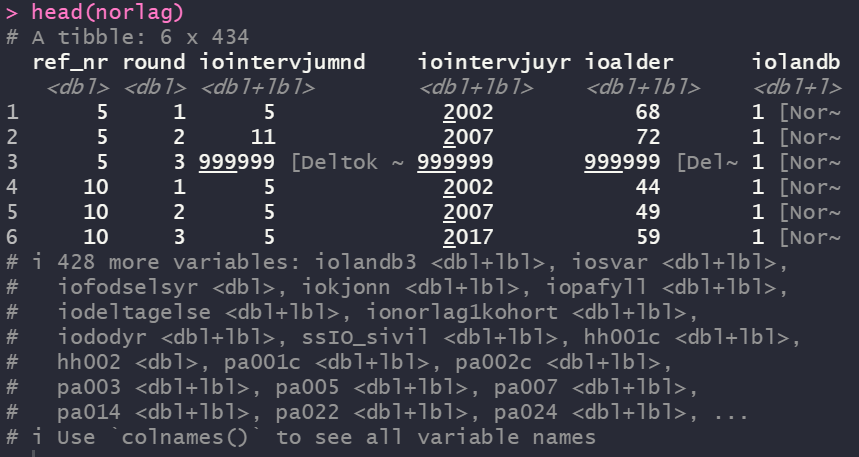
\includegraphics{./images/head_skjermdump.png}

Legg merke til at under hvert variabelnavn er det en indikasjon på hva
slags variabeltype det er. For eksempel betyr
\texttt{\textless{}dbl\textgreater{}} at det er en numerisk variabel
mens \texttt{\textless{}dbl+lbl\textgreater{}} indikerer at variabelen
inneholder \emph{labels}.

Det er lite hensiktsmessig å vise alt i konsollen fordi det rett og
slett ikke er plass. Nerst står det derfor angitt at det er flere
variable som ikke vises og navnet på de første av disse.

\hypertarget{subset-med-klammeparenteser}{%
\subsection{Subset med
klammeparenteser}\label{subset-med-klammeparenteser}}

En enkel løsning er å bare se på noen få variable om gangen. Med
klammeparentes kan vi angi hvilke radnummer og kolonnenummer vi ønsker
se på med følgende syntax: \texttt{datasett{[}rader,\ kolonner{]}} der
altså komma skiller mellom rader og kolonner. Følgende eksempel viser
hvordan man kan bruke \texttt{head()} for å vise de første
observasjonene i datasettet med bare de første 5 variablene (altså:
kollonne nr 1-5).

\begin{Shaded}
\begin{Highlighting}[]
\FunctionTok{head}\NormalTok{(norlag[, }\DecValTok{1}\SpecialCharTok{:}\DecValTok{5}\NormalTok{])}
\end{Highlighting}
\end{Shaded}

\begin{verbatim}
  ref_nr         iodeltakelse iododaar iofodselsaar iokjonn
1      5     Deltatt T1 og T2     <NA>         1934    Mann
2      5     Deltatt T1 og T2     <NA>         1934    Mann
3     10 Deltatt T1, T2 og T3     <NA>         1957  Kvinne
4     10 Deltatt T1, T2 og T3     <NA>         1957  Kvinne
5     10 Deltatt T1, T2 og T3     <NA>         1957  Kvinne
6     12     Deltatt T1 og T3     <NA>         1955  Kvinne
\end{verbatim}

Vi kan altså også angi både rader og kollonner på denne måten. Her er
eksempel som viser første 3 rader og variabelnummer 40 til 44.

\begin{Shaded}
\begin{Highlighting}[]
\FunctionTok{head}\NormalTok{(norlag[}\DecValTok{1}\SpecialCharTok{:}\DecValTok{3}\NormalTok{, }\DecValTok{40}\SpecialCharTok{:}\DecValTok{44}\NormalTok{])}
\end{Highlighting}
\end{Shaded}

\begin{verbatim}
  hc201 hc202 hc203 hc204 hc205
1   176    85    Ja   Nei    Ja
2   176    95    Ja   Nei    Ja
3   168    64    Ja   Nei    Ja
\end{verbatim}

Legg merke til at under hvert variabelnavn står det en liten tekst,
f.eks. eller \textless S3: haven\_labelled\textgreater. Det kan også stå
andre ting. dbl betyr at det er en kontinuerlig variabel, mens
haven\_labelled betyr at det er labler til alle eller noe verdier i
variabelen.

Vi skal primært jobbe med data som ikke er ``labelled'', men du vil noen
ganger komme borti dette, spesielt hvis du importerer data fra andre
statistikksoftware.

\hypertarget{bruke-glimpse}{%
\subsection{Bruke `glimpse()'}\label{bruke-glimpse}}

I tidligere kurs skal dere ha lært å bruke funksjonen
\texttt{glimpse()}, men også her blir det mest rotete fordi det er så
mange variable. Det tar rett og slett veldig stor plass på skjermen.

En variant er å bruke \texttt{glimpse()} bare på et utvalg variable på
tilsvarende måte. Her er et eksempel, men der vi ser på de 20 første
variablene ved bruk av klammeparentes tilsvarende som vist over.

\begin{Shaded}
\begin{Highlighting}[]
\FunctionTok{glimpse}\NormalTok{(norlag[, }\DecValTok{1}\SpecialCharTok{:}\DecValTok{20}\NormalTok{])}
\end{Highlighting}
\end{Shaded}

\begin{verbatim}
Rows: 20,892
Columns: 20
$ ref_nr          <dbl> 5, 5, 10, 10, 10, 12, 12, 15, 15, 18, 18, 22, 23, 23, ~
$ iodeltakelse    <fct> "Deltatt T1 og T2", "Deltatt T1 og T2", "Deltatt T1, T~
$ iododaar        <fct> NA, NA, NA, NA, NA, NA, NA, NA, NA, NA, NA, 2006, NA, ~
$ iofodselsaar    <dbl> 1934, 1934, 1957, 1957, 1957, 1955, 1955, 1944, 1944, ~
$ iokjonn         <fct> Mann, Mann, Kvinne, Kvinne, Kvinne, Kvinne, Kvinne, Kv~
$ ionorlag1kohort <fct> Del av NorLAG1 kohort, Del av NorLAG1 kohort, Del av N~
$ iopafyll        <fct> Ingen påfyll, Ingen påfyll, Ingen påfyll, Ingen påfyll~
$ iovektnorlag2   <fct> 143, 143, 51, 51, 51, NA, NA, 195, 195, 215, 215, NA, ~
$ iovektnorlag3   <fct> NA, NA, 73, 73, 73, 135, 135, NA, NA, 227, 227, NA, 39~
$ pr002c          <fct> 1905, 1905, 1933, 1933, 1933, 1918, 1918, 1918, 1918, ~
$ pr003c          <fct> 1991, 1991, NA, NA, NA, 2004, 2004, 1989, 1989, NA, NA~
$ pr005c          <fct> 1905, 1905, 1933, 1933, 1933, 1915, 1915, 1909, 1909, ~
$ pr006c          <fct> 1996, 1996, NA, NA, NA, 1996, 1996, 1975, 1975, 1976, ~
$ pr007c          <fct> Grunnskole, Grunnskole, Videregående, Videregående, Vi~
$ pr011c          <fct> Videregående, Videregående, Grunnskole, Grunnskole, Gr~
$ round           <dbl> 1, 2, 3, 2, 1, 3, 1, 1, 2, 3, 2, 1, 3, 1, 1, 3, 2, 1, ~
$ ioalder         <fct> 68, 72, 59, 49, 44, 61, 47, 58, 63, 67, 57, 63, 69, 55~
$ iointervjumnd   <fct> 5, 11, 5, 5, 5, 8, 5, 8, 3, 3, 5, 8, 5, 8, 2, 5, 9, 4,~
$ iointervjuaar   <fct> 2002, 2007, 2017, 2007, 2002, 2017, 2002, 2002, 2007, ~
$ iolandb         <fct> NA, Norskfødt, NA, Norskfødt, NA, NA, NA, NA, Norskfød~
\end{verbatim}

I denne output'en er den første kollonnen altså variabelnavnene,
deretter er det en kollonne som viser hva slags type variabel det er, og
deretter de første observasjonene på hver variabel slik at man får et
inntrykk av hvordan det ser ut. \texttt{glimpse()} gir altså omtrent
samme informasjon som \texttt{head()}, men er nok mer hensiktsmessig
hvis mange variable.

\hypertarget{undersuxf8ke-enkeltvariable-med-codebook-fra-pakken-memisc}{%
\subsection{\texorpdfstring{Undersøke enkeltvariable med
\texttt{codebook()} fra pakken
\{memisc\}}{Undersøke enkeltvariable med codebook() fra pakken \{memisc\}}}\label{undersuxf8ke-enkeltvariable-med-codebook-fra-pakken-memisc}}

Noen ganger vil man ha litt mer informasjon om enkeltvariablene. Noen
datasett vil komme med labler (omtalt annet sted) eller faktorvariable,
som gjør at variablene inneholder både tallverdier og tekst.

Å få ut noe deskriptiv statistikk og se på fordelinger er da gjerne
neste steg som vil bli behandlet i de etterfølgende kapitlene.

Man vil klare seg greit med det vi har vist ovenfor. Men det finnes
flere måter å gjøre det på. Pakken \{memisc\} inneholder en rekke
funksjoner for å håndtere surveydata, som vi ikke skal gå nærmere inn på
her. Men akkurat funksjonen \texttt{codebook()} gir litt mer informativt
output enn \texttt{look\_for()}.

For å bruke denne må du installere pakken først. I eksempelet nedenfor
er pakken ikke lastet med library(), men angitt pakken direkte med
\texttt{memisc::} først. Dette kan være nyttig hvis man ikke skal bruke
noen andre funksjoner fra denne pakken.

\begin{Shaded}
\begin{Highlighting}[]
\NormalTok{memisc}\SpecialCharTok{::}\FunctionTok{codebook}\NormalTok{(norlag}\SpecialCharTok{$}\NormalTok{iokjonn)}
\end{Highlighting}
\end{Shaded}

\begin{verbatim}
================================================================================

   norlag$iokjonn 'IOs kjønn'

--------------------------------------------------------------------------------

   Storage mode: integer
   Factor with 2 levels

   Levels and labels     N Valid
                                
   1 'Mann'          10244  49.0
   2 'Kvinne'        10648  51.0
\end{verbatim}

Poenget her er altså bare å få en penere output og litt deskriptiv
statistikk samtidig.

\hypertarget{suxf8ke-i-datasettet-etter-variable}{%
\section{Søke i datasettet etter
variable}\label{suxf8ke-i-datasettet-etter-variable}}

For å se nærmere på en variabel går an å bruke funksjonen
\texttt{look\_for()}, som primært er en søke-funksjon, men det gir også
informasjon om variabelen.

\begin{Shaded}
\begin{Highlighting}[]
\FunctionTok{look\_for}\NormalTok{(norlag, }\StringTok{"iokjonn"}\NormalTok{)}
\end{Highlighting}
\end{Shaded}

\begin{verbatim}
 pos variable label     col_type values
 5   iokjonn  IOs kjønn fct      Mann  
                                 Kvinne
\end{verbatim}

I output fremgår det at dette er den 10'ende variabelen, inneholder
informasjonen ``IOs kjønn'', er av typen numerisk med tilhørende labler,
og verdiene er 1 = Mann og 2 = Kvinne.

Det går også an å bare få ut variabel-label med funksjonen
\texttt{var\_label()} slik:

\begin{Shaded}
\begin{Highlighting}[]
\FunctionTok{var\_label}\NormalTok{(norlag}\SpecialCharTok{$}\NormalTok{iokjonn)}
\end{Highlighting}
\end{Shaded}

\begin{verbatim}
[1] "IOs kjønn"
\end{verbatim}

For å se labels på \emph{verdiene} bruk \textbf{val\_labels()}.

\begin{Shaded}
\begin{Highlighting}[]
\FunctionTok{val\_labels}\NormalTok{(norlag}\SpecialCharTok{$}\NormalTok{iokjonn)}
\end{Highlighting}
\end{Shaded}

\begin{verbatim}
NULL
\end{verbatim}

Alle datasett skal komme med en dokumentasjon som sier hva hver variabel
inneholder og hvilke verdier som finnes i hver variable, og hva de
betyr. Dette leveres gjerne som en separat fil, ganske ofte i pdf eller
html format. NSD/Sikt leverer dokumentasjonen for Norlag i html-format.
(Ideelt burde det vært i et enkelt maskinlesbart format egnet til å
bruke til omkoding og labler for de som ønsker det, men de har valgt en
annen løsning).

Du kan søke i dokumentasjonen på samme måte som i andre filer, men det
kan være litt knotete. Et godt alternativ er å søke direkte i
datasettet. Funksjonen \texttt{look\_for()} søker både i variabelnavn,
verdier og labler. Her er et eksempel for hvordan finne variabler som
inneholder ordet ``yrkesinntekt''. Du kan også søke på kortere eller
lengre tekststrenger. (Søker du f.eks. bare på ``innt'' eller ``yrke''
så får du opp langt flere variable, så du må kanskje prøve deg litt
frem).

\begin{Shaded}
\begin{Highlighting}[]
\FunctionTok{look\_for}\NormalTok{(norlag, }\StringTok{"Yrkesinntekt"}\NormalTok{)}
\end{Highlighting}
\end{Shaded}

Det er to variable som inneholder teksten ``yrkesinntekt''. Den første
variabelen har posisjon 353 i datasettet og har variabelnavnet
inwyrkinnt. Den andre variabelen har posisjon 371 og har navnet
inpartwyrkinnt. Vi fokuserer på den første.

Merk at når labelen avsluttes med \textasciitilde{} (uttales ``tilde'')
indikerer det at teksten er avkortet i outputvinduet. Du får opp hele
teksten ved å bruke \texttt{val\_label()} slik:

\begin{Shaded}
\begin{Highlighting}[]
\FunctionTok{var\_label}\NormalTok{(norlag}\SpecialCharTok{$}\NormalTok{inwyrkinnt)}
\end{Highlighting}
\end{Shaded}

\begin{verbatim}
NULL
\end{verbatim}

\part{Del 2: Deskriptive teknikker}

\hypertarget{grafikk-med-ggplot}{%
\chapter{Grafikk med ggplot}\label{grafikk-med-ggplot}}

Resten av dette heftet belager seg på å bruke datasettet abu89 som er
benyttet i en annen lærebok. Dataene kan lastes ned fra
\href{https://stata.fagbokforlaget.no/}{den bokens hjemmeside}.

Først må dataene leses inn. Siden dette er data i stata-formatet dta, så
brukes importfunksjonen \texttt{read\_stata()}. Som nevnt tidligere bør
variabler av typen labelled gjøres om til factor. Vi sletter også labler
som ikke er i faktisk bruk. Disse to tingene gjørs med
\texttt{as\_factor()} og \texttt{fct\_drop()}, men de er lagt inn i en
funksjon som går gjennom alle variable i datasettet, \texttt{across()}
og sjekker om de er av labelled-typen \texttt{where(is.labelled)}.
Detaljene her er ikke sentrale for dette kurset: bare se å få lest inn
dataene i R.

\begin{Shaded}
\begin{Highlighting}[]
\FunctionTok{library}\NormalTok{(haven)}
\FunctionTok{library}\NormalTok{(tidyverse)}

\NormalTok{abu89 }\OtherTok{\textless{}{-}} \FunctionTok{read\_stata}\NormalTok{(}\StringTok{"data/abu89.dta"}\NormalTok{) }\SpecialCharTok{\%\textgreater{}\%} 
  \FunctionTok{mutate}\NormalTok{(}\FunctionTok{across}\NormalTok{(}\FunctionTok{where}\NormalTok{(is.labelled), }\SpecialCharTok{\textasciitilde{}}\FunctionTok{as\_factor}\NormalTok{(.)),}
         \FunctionTok{across}\NormalTok{(}\FunctionTok{where}\NormalTok{(is.factor), }\SpecialCharTok{\textasciitilde{}}\FunctionTok{fct\_drop}\NormalTok{(.)))}

\FunctionTok{glimpse}\NormalTok{(abu89)}
\end{Highlighting}
\end{Shaded}

\begin{verbatim}
Rows: 4,127
Columns: 9
$ io_nr    <dbl> 3, 4, 5, 8, 11, 12, 13, 14, 16, 17, 18, 19, 20, 21, 22, 23, 2~
$ time89   <dbl> 62.00000, NA, 91.32895, 84.23913, 90.42553, 103.28947, 75.000~
$ ed       <dbl> 0, 1, 3, 5, 3, 1, 1, 7, 3, 9, 0, 9, 1, 3, 9, 3, 0, 3, 1, 3, 3~
$ age      <dbl> 58, 24, 44, 46, 40, 36, 31, 31, 26, 29, 54, 58, 25, 25, 56, 5~
$ female   <dbl> 1, 0, 1, 1, 0, 0, 1, 0, 0, 0, 1, 0, 0, 0, 0, 0, 1, 0, 0, 1, 1~
$ klasse89 <fct> III Rutinefunksjonærer, VIIa Ufaglærte arbeidere, II Nedre se~
$ promot   <fct> NEI, JA, JA, NEI, NEI, NEI, NEI, NEI, JA, NEI, JA, JA, NEI, J~
$ fexp     <dbl> 1.0, 0.3, 1.9, 0.3, 1.0, 1.2, 0.1, 0.4, 0.2, 0.3, 3.5, 3.1, 0~
$ private  <fct> Public, Private, Private, Public, Private, Public, Public, Pr~
\end{verbatim}

\hypertarget{lagvis-grafikk}{%
\section{Lagvis grafikk}\label{lagvis-grafikk}}

I R er det mange funksjoner for å lage grafikk. Noen er spesialiserte og
knyttet til spesielle analysemetoder og gir deg akkurat det du trenger.
Vi skal her bruke et \emph{generelt system} for grafikk som heter
\texttt{ggplot} som kan brukes til all slags grafikk. Funksjonen
\emph{ggplot} er bygget opp som en \emph{gramatikk} for grafisk
fremstilling. Det ligger en teori til grunn som er utledet i boken ved
omtrent samme navn:
\href{https://link.springer.com/book/10.1007/0-387-28695-0}{The grammar
of graphics}. Det er mye som kan sies om dette, men det viktige er at
grafikken er bygget opp rundt noen bestanddeler. Når du behersker disse
kan du fremstille nær sagt hva som helst av kvantitativ informasjon
grafisk. Dette er altså et system for grafikk, ikke bare kommandoer for
spesifikke typer plot. Vi skal likevel bare se på grunnleggende typer
plot her.

Systemet er bygd opp \emph{lagvis}. Det gjelder selve koden, men også
hvordan det ser ut visuelt. Man kan utvide plottet med flere lag i samme
plot og det legges da oppå hverandre i den rekkefølgen som angis i
koden.

For enkle plot som vi skal bruke her angir man i denne rekkefølgen og
med en \texttt{+} mellom hver del (vanligvis per linje, men linjeskift
spiller ingen rolle). Hver del av koden spesifiserer enten \emph{hva}
som skal plottes eller \emph{hvordan} det plottes, mens andre deler kan
kontrollere utseende på akser, fargeskalaer, støttelinjer eller andre
ting som har med layout å gjøre.

\begin{enumerate}
\def\labelenumi{\arabic{enumi})}
\tightlist
\item
  Angi data og \emph{hva} som skal plottes med \texttt{ggplot()}
\item
  Angi \emph{hvordan} det skal plottes med \texttt{geom\_*()}
\item
  Angi andre spesifikasjoner (farger, titler, koordinatsystemer osv)
\end{enumerate}

Dette blir tydeligere i eksemplene og forklares underveis.

\begin{itemize}
\tightlist
\item
  Det første argumentet i \texttt{ggplot} er data. Altså: hvilket
  datasett informasjonen hentes fra.
\item
  Inni \texttt{ggplot()} må det spesifiseres \texttt{aes()},
  ``\emph{aestethics}'', som er \emph{hvilke variable} som skal plottes.
  Først og fremst hva som skal på x-akse og y-akse (og evt. z-akse), men
  også spesifikasjon av om linjer (farge, linjetype) og fyllfarger, skal
  angis etter en annen variabel.
\item
  \texttt{geom\_*} står for \emph{geometric} og sier noe om
  \emph{hvordan} data skal se ut. Det kan være punkter, histogram,
  stolper, linjer osv.
\item
  \texttt{coord\_*} definerer koordinatsystemet. Stort sett blir dette
  bestemt av variablene. Men du kan også snu grafen eller definere
  sirkulært koordinatsystem, eller andre enklere ting.
\item
  \texttt{facet\_*} definerer hvordan du vil dele opp grafikken i
  undergrupper
\end{itemize}

\hypertarget{kategoriske-variabel}{%
\section{Kategoriske variabel}\label{kategoriske-variabel}}

\hypertarget{stolpediagram}{%
\subsection{Stolpediagram}\label{stolpediagram}}

\begin{Shaded}
\begin{Highlighting}[]
\FunctionTok{library}\NormalTok{(ggforce)}
\FunctionTok{ggplot}\NormalTok{(abu89, }\FunctionTok{aes}\NormalTok{(}\AttributeTok{x =}\NormalTok{ klasse89)) }\SpecialCharTok{+}
  \FunctionTok{geom\_bar}\NormalTok{() }\SpecialCharTok{+}
  \FunctionTok{theme}\NormalTok{(}\AttributeTok{axis.text.x =} \FunctionTok{element\_text}\NormalTok{(}\AttributeTok{angle =} \DecValTok{90}\NormalTok{))}
\end{Highlighting}
\end{Shaded}

\begin{figure}[H]

{\centering \includegraphics{./grafikk_files/figure-pdf/unnamed-chunk-2-1.pdf}

}

\end{figure}

Noen ganger ønsker man å vise fordelingen for to ulike grupper, la oss
si for kjønn. En mulighet er da å rett og slett lage to stolpediagram
ved siden av hverandre. Til dette kan man spesifisere at dataene er
gruppert etter variabelen \emph{female} og at fyllfargen skal settes
etter denne variablen med \texttt{fill\ =\ factor(female)}. Merk bruken
av \texttt{factor(female)} fordi variabelen er \emph{numerisk} og det
vil da ellers brukes en kontinuerlig fargeskale, mens å gjøre om
variabelen til kategorisk brukes en annen fargeskala.

I tillegg gjør vi her to ting til: setter et annet grafisk tema med
\texttt{theme\_minimal()} og snur plotvinduet slik at kategoriene er
litt lettere å lese. Dette er smak og behag.

\begin{Shaded}
\begin{Highlighting}[]
\FunctionTok{ggplot}\NormalTok{(abu89, }\FunctionTok{aes}\NormalTok{(}\AttributeTok{x =}\NormalTok{ klasse89, }\AttributeTok{group =}\NormalTok{ female, }\AttributeTok{fill =} \FunctionTok{factor}\NormalTok{(female))) }\SpecialCharTok{+}
  \FunctionTok{geom\_bar}\NormalTok{(}\AttributeTok{position=}\StringTok{"dodge"}\NormalTok{) }\SpecialCharTok{+}
  \FunctionTok{theme\_minimal}\NormalTok{()}\SpecialCharTok{+}
  \FunctionTok{theme}\NormalTok{(}\AttributeTok{axis.text.x =} \FunctionTok{element\_text}\NormalTok{(}\AttributeTok{angle =} \DecValTok{90}\NormalTok{))}\SpecialCharTok{+}
  \FunctionTok{coord\_flip}\NormalTok{()}
\end{Highlighting}
\end{Shaded}

\begin{figure}[H]

{\centering 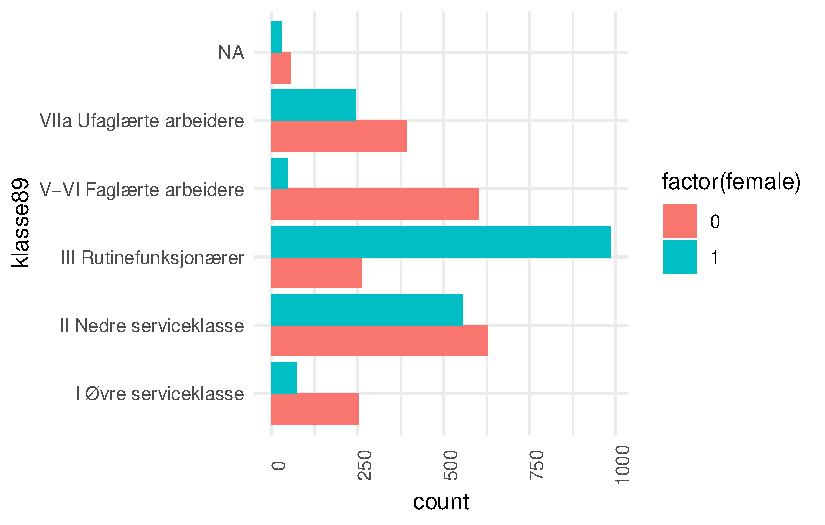
\includegraphics{./grafikk_files/figure-pdf/unnamed-chunk-3-1.pdf}

}

\end{figure}

Et alternativ er å plassere grafikken for menn og kvinner ved siden av
hverandre. Å legge til \texttt{facet\_wrap()} gjør dette.

\begin{Shaded}
\begin{Highlighting}[]
\FunctionTok{ggplot}\NormalTok{(abu89, }\FunctionTok{aes}\NormalTok{(}\AttributeTok{x =}\NormalTok{ klasse89)) }\SpecialCharTok{+}
  \FunctionTok{geom\_bar}\NormalTok{() }\SpecialCharTok{+}
  \FunctionTok{facet\_wrap}\NormalTok{(}\SpecialCharTok{\textasciitilde{}}\FunctionTok{factor}\NormalTok{(female)) }\SpecialCharTok{+}
  \FunctionTok{theme}\NormalTok{(}\AttributeTok{axis.text.x =} \FunctionTok{element\_text}\NormalTok{(}\AttributeTok{angle =} \DecValTok{90}\NormalTok{))}
\end{Highlighting}
\end{Shaded}

\begin{figure}[H]

{\centering \includegraphics{./grafikk_files/figure-pdf/unnamed-chunk-4-1.pdf}

}

\end{figure}

Et automatisk forvalg for \texttt{geom\_bar()} er hvordan gruppene
plasseres som er \texttt{position="stack"}. Det betyr at gruppene
stables oppå hverandre. Dette er godt egnet hvis poenget er å vise hvor
mange av hvert kjønn som er i hver gruppe. Det er mindre egnet hvis du
ønsker å sammenligne menn og kvinner. Da er alternativet å velge
\texttt{position="dodge"} som følger:

\hypertarget{kakediagram}{%
\subsection{Kakediagram}\label{kakediagram}}

Generelt er ikke kakediagram å anbefale da korrekt tolkning involverer å
tolke et areal som inneholder vinkel. Med få kategorier som er rimelig
forskjellig kan det gi et ok inntrykk, men ofte ender man opp med å
måtte skrive på tallene likevel. Vi tar det med her egentlig bare fordi
mange insisterer på å bruke det. Så vet du at det er mulig.

Det enkleste er å bruke funksjonen \texttt{pie()} som gir følgende
resultat.

\begin{Shaded}
\begin{Highlighting}[]
\NormalTok{tab }\OtherTok{\textless{}{-}} \FunctionTok{table}\NormalTok{(abu89}\SpecialCharTok{$}\NormalTok{klasse89) }
\NormalTok{tab}
\end{Highlighting}
\end{Shaded}

\begin{verbatim}

    I Øvre serviceklasse   II Nedre serviceklasse   III Rutinefunksjonærer 
                     328                     1181                     1248 
 V-VI Faglærte arbeidere VIIa Ufaglærte arbeidere 
                     648                      637 
\end{verbatim}

\begin{Shaded}
\begin{Highlighting}[]
\FunctionTok{pie}\NormalTok{(tab)}
\end{Highlighting}
\end{Shaded}

\begin{figure}[H]

{\centering 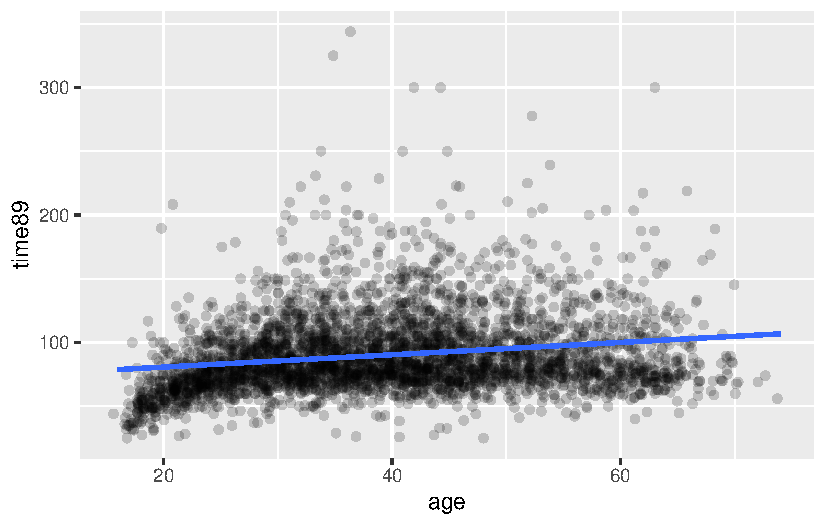
\includegraphics{./grafikk_files/figure-pdf/unnamed-chunk-5-1.pdf}

}

\end{figure}

Men hvis man skal bruke ggplot er det litt mer jobb. Fordelen med ggplot
er at du har bedre kontroll for å lage publiserbar kvalitet. (Akkurat
for kakediagram er det kanskje ikke så farlige, for du bør ikke bruke
det i publikasjoner hvis du kan la være).

\begin{Shaded}
\begin{Highlighting}[]
\NormalTok{pc }\OtherTok{\textless{}{-}}\NormalTok{ abu89 }\SpecialCharTok{\%\textgreater{}\%} 
  \FunctionTok{group\_by}\NormalTok{(klasse89) }\SpecialCharTok{\%\textgreater{}\%} 
  \FunctionTok{summarise}\NormalTok{(}\AttributeTok{n =} \FunctionTok{n}\NormalTok{()) }\SpecialCharTok{\%\textgreater{}\%} 
  \FunctionTok{mutate}\NormalTok{(}\AttributeTok{pct =}\NormalTok{ n}\SpecialCharTok{/}\FunctionTok{sum}\NormalTok{(n)}\SpecialCharTok{*}\DecValTok{100}\NormalTok{) }\SpecialCharTok{\%\textgreater{}\%} 
  \FunctionTok{ungroup}\NormalTok{()}

\FunctionTok{ggplot}\NormalTok{(pc, }\FunctionTok{aes}\NormalTok{(}\AttributeTok{x =} \StringTok{""}\NormalTok{, }\AttributeTok{y =}\NormalTok{ pct, }\AttributeTok{fill =}\NormalTok{ (klasse89))) }\SpecialCharTok{+}
  \FunctionTok{geom\_bar}\NormalTok{(}\AttributeTok{stat=}\StringTok{"identity"}\NormalTok{, }\AttributeTok{width=}\DecValTok{1}\NormalTok{) }\SpecialCharTok{+}
  \FunctionTok{coord\_polar}\NormalTok{(}\StringTok{"y"}\NormalTok{, }\AttributeTok{start=}\DecValTok{0}\NormalTok{) }\SpecialCharTok{+}
  \FunctionTok{theme\_void}\NormalTok{()}\SpecialCharTok{+}
  \FunctionTok{geom\_text}\NormalTok{( }\FunctionTok{aes}\NormalTok{(}\AttributeTok{label =} \FunctionTok{paste0}\NormalTok{( }\FunctionTok{round}\NormalTok{(pct,}\DecValTok{1}\NormalTok{), }\StringTok{"\%"}\NormalTok{), }\AttributeTok{x =} \FloatTok{1.4}\NormalTok{), }
            \AttributeTok{position =} \FunctionTok{position\_stack}\NormalTok{(}\AttributeTok{vjust=}\NormalTok{.}\DecValTok{5}\NormalTok{), }\AttributeTok{check\_overlap =}\NormalTok{ F) }\SpecialCharTok{+}
  \FunctionTok{labs}\NormalTok{(}\AttributeTok{x =} \ConstantTok{NULL}\NormalTok{, }\AttributeTok{y =} \ConstantTok{NULL}\NormalTok{, }\AttributeTok{fill =} \ConstantTok{NULL}\NormalTok{)}\SpecialCharTok{+}
  \FunctionTok{theme}\NormalTok{(}\AttributeTok{axis.line =} \FunctionTok{element\_blank}\NormalTok{(),}
          \AttributeTok{axis.text =} \FunctionTok{element\_blank}\NormalTok{(),}
          \AttributeTok{axis.ticks =} \FunctionTok{element\_blank}\NormalTok{()) }\SpecialCharTok{+}
  \FunctionTok{scale\_fill\_brewer}\NormalTok{(}\AttributeTok{palette=}\StringTok{"Blues"}\NormalTok{, }\AttributeTok{direction =} \SpecialCharTok{{-}}\DecValTok{1}\NormalTok{)}
\end{Highlighting}
\end{Shaded}

\begin{figure}[H]

{\centering 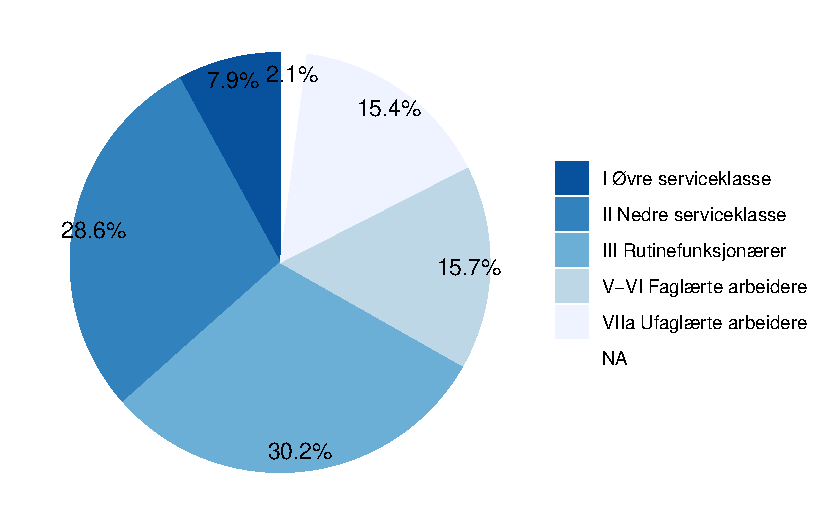
\includegraphics{./grafikk_files/figure-pdf/unnamed-chunk-6-1.pdf}

}

\end{figure}

\hypertarget{kontinuerlige-variable}{%
\section{Kontinuerlige variable}\label{kontinuerlige-variable}}

\hypertarget{histogram}{%
\subsection{Histogram}\label{histogram}}

\begin{Shaded}
\begin{Highlighting}[]
\FunctionTok{ggplot}\NormalTok{(abu89, }\FunctionTok{aes}\NormalTok{(}\AttributeTok{x =}\NormalTok{ time89)) }\SpecialCharTok{+}
  \FunctionTok{geom\_histogram}\NormalTok{()}
\end{Highlighting}
\end{Shaded}

\begin{figure}[H]

{\centering 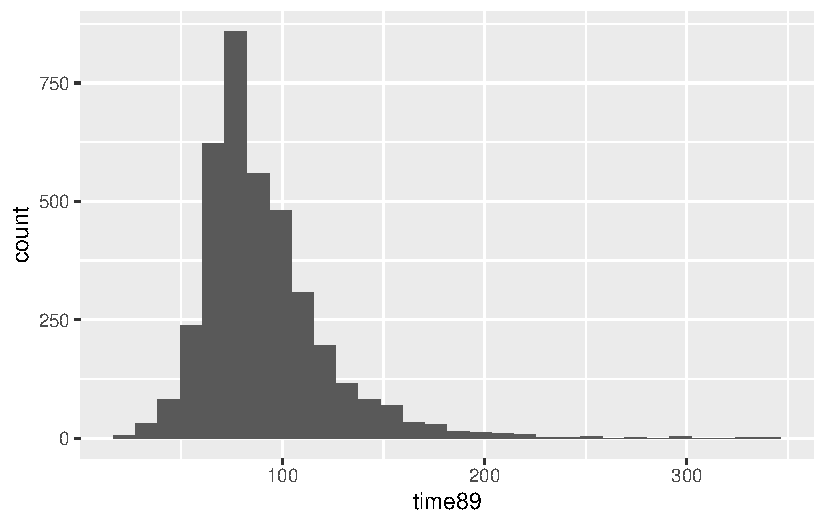
\includegraphics{./grafikk_files/figure-pdf/unnamed-chunk-7-1.pdf}

}

\end{figure}

Det er også vanlig å fremstille det samme på en ``tetthetsskala'', der
arealet summeres til 1. Det betyr at arealet for hvert intervall
tilsvarer en andel. Visuelt sett er det vel så mye arealet vi oppfatter
som høyden på stolpene. Men det er bare skalaen på y-aksen som har
endret seg. Visuelt sett, ser histogrammene helt like ut.

\begin{Shaded}
\begin{Highlighting}[]
\FunctionTok{ggplot}\NormalTok{(abu89, }\FunctionTok{aes}\NormalTok{(}\AttributeTok{x =}\NormalTok{ time89, }\AttributeTok{y =}\NormalTok{ ..density..)) }\SpecialCharTok{+}
  \FunctionTok{geom\_histogram}\NormalTok{()}
\end{Highlighting}
\end{Shaded}

\begin{figure}[H]

{\centering 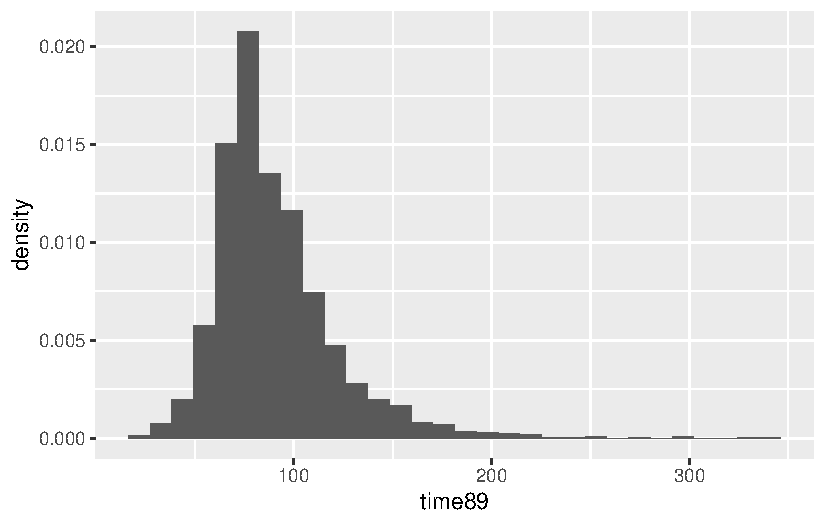
\includegraphics{./grafikk_files/figure-pdf/unnamed-chunk-8-1.pdf}

}

\end{figure}

\hypertarget{density-plot}{%
\subsection{Density plot}\label{density-plot}}

Density plot er en måte å fremstille det samme på, men i stedet for å
dele inn i intervaller som i histogram lager vi en glattet kurve. Det
blir på skalaen ``tetthet'' som i histogrammet ovenfor.

\begin{Shaded}
\begin{Highlighting}[]
\FunctionTok{ggplot}\NormalTok{(abu89, }\FunctionTok{aes}\NormalTok{(}\AttributeTok{x =}\NormalTok{ time89)) }\SpecialCharTok{+}
  \FunctionTok{geom\_density}\NormalTok{()}
\end{Highlighting}
\end{Shaded}

\begin{figure}[H]

{\centering 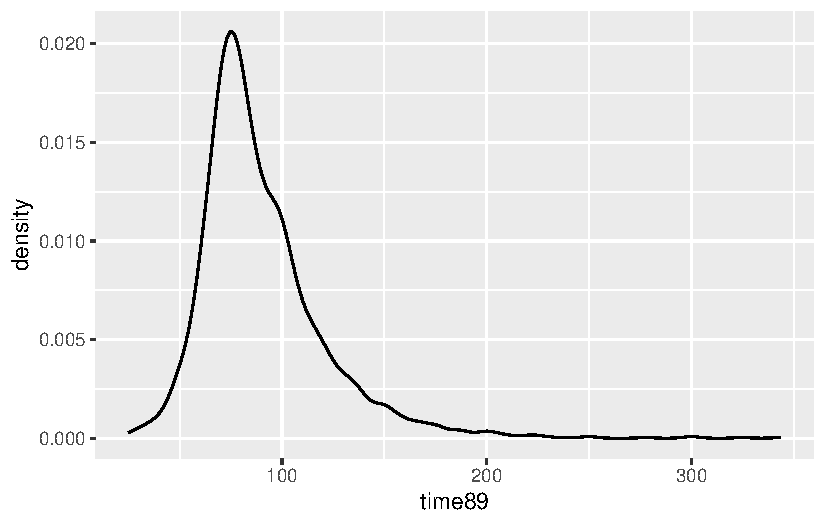
\includegraphics{./grafikk_files/figure-pdf/unnamed-chunk-9-1.pdf}

}

\end{figure}

\begin{Shaded}
\begin{Highlighting}[]
\FunctionTok{ggplot}\NormalTok{(abu89, }\FunctionTok{aes}\NormalTok{(}\AttributeTok{x =}\NormalTok{ time89)) }\SpecialCharTok{+}
  \FunctionTok{geom\_histogram}\NormalTok{(}\FunctionTok{aes}\NormalTok{(}\AttributeTok{y =}\NormalTok{ ..density..), }\AttributeTok{fill =} \StringTok{"lightgrey"}\NormalTok{, }\AttributeTok{col =} \StringTok{"grey"}\NormalTok{) }\SpecialCharTok{+}
  \FunctionTok{geom\_density}\NormalTok{(}\AttributeTok{col =} \StringTok{"red"}\NormalTok{, }\AttributeTok{linewidth =} \DecValTok{1}\NormalTok{) }\SpecialCharTok{+}
  \FunctionTok{theme\_minimal}\NormalTok{()}
\end{Highlighting}
\end{Shaded}

\begin{figure}[H]

{\centering 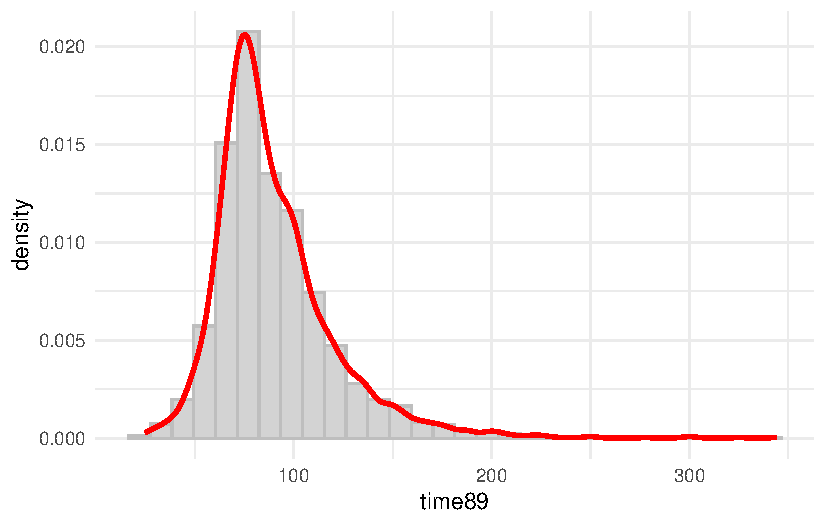
\includegraphics{./grafikk_files/figure-pdf/unnamed-chunk-10-1.pdf}

}

\end{figure}

En fordel med denne fremstillingen er at det er lettere å sammenligne
grupper. Her er et eksempel med density plot etter hvor mye man drikker.

\begin{Shaded}
\begin{Highlighting}[]
\FunctionTok{ggplot}\NormalTok{(abu89, }\FunctionTok{aes}\NormalTok{(}\AttributeTok{x =}\NormalTok{ time89, }\AttributeTok{group =}\NormalTok{ klasse89, }\AttributeTok{linetype =}\NormalTok{ klasse89)) }\SpecialCharTok{+}
  \FunctionTok{geom\_density}\NormalTok{(}\AttributeTok{linewidth =} \DecValTok{1}\NormalTok{)}\SpecialCharTok{+}
  \FunctionTok{guides}\NormalTok{(}\AttributeTok{fill =} \FunctionTok{guide\_legend}\NormalTok{(}\AttributeTok{override.aes =} \FunctionTok{list}\NormalTok{(}\AttributeTok{shape =} \DecValTok{1}\NormalTok{ ) ) ) }\SpecialCharTok{+}
  \FunctionTok{theme\_minimal}\NormalTok{()}
\end{Highlighting}
\end{Shaded}

\begin{figure}[H]

{\centering 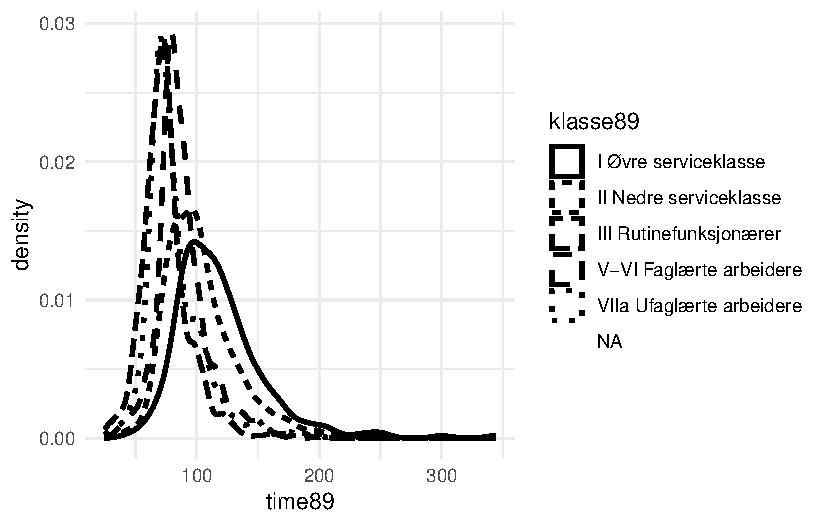
\includegraphics{./grafikk_files/figure-pdf/unnamed-chunk-11-1.pdf}

}

\end{figure}

\begin{Shaded}
\begin{Highlighting}[]
\FunctionTok{ggplot}\NormalTok{(abu89, }\FunctionTok{aes}\NormalTok{(}\AttributeTok{x =}\NormalTok{ time89)) }\SpecialCharTok{+}
  \FunctionTok{geom\_density}\NormalTok{(}\AttributeTok{linewidth =} \DecValTok{1}\NormalTok{)}\SpecialCharTok{+}
  \FunctionTok{theme\_minimal}\NormalTok{()}\SpecialCharTok{+}
  \FunctionTok{facet\_wrap}\NormalTok{(}\SpecialCharTok{\textasciitilde{}}\NormalTok{klasse89, }\AttributeTok{scales=}\StringTok{"free"}\NormalTok{)}
\end{Highlighting}
\end{Shaded}

\begin{figure}[H]

{\centering 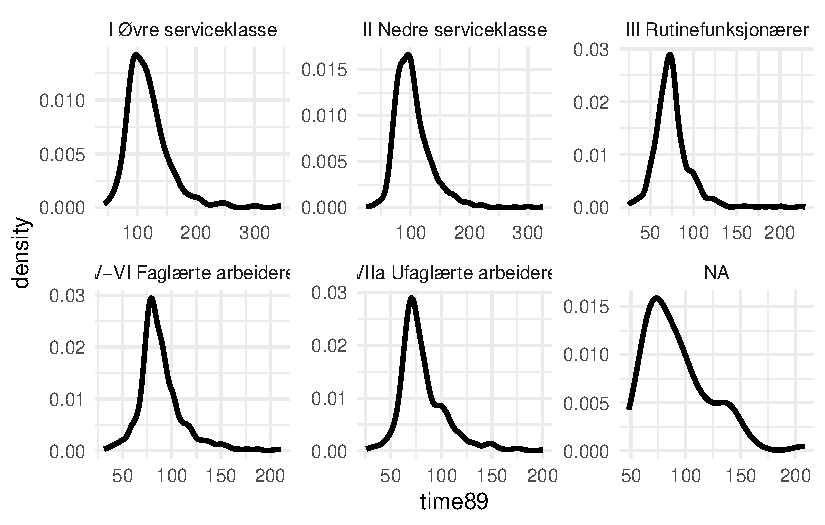
\includegraphics{./grafikk_files/figure-pdf/unnamed-chunk-12-1.pdf}

}

\end{figure}

\begin{Shaded}
\begin{Highlighting}[]
\FunctionTok{ggplot}\NormalTok{(abu89, }\FunctionTok{aes}\NormalTok{(}\AttributeTok{x =}\NormalTok{ time89, }\AttributeTok{group =}\NormalTok{ female,  }\AttributeTok{fill =} \FunctionTok{factor}\NormalTok{(female))) }\SpecialCharTok{+}
  \FunctionTok{geom\_density}\NormalTok{(}\AttributeTok{alpha =}\NormalTok{ .}\DecValTok{3}\NormalTok{)}\SpecialCharTok{+}
  \FunctionTok{guides}\NormalTok{(}\AttributeTok{fill=}\FunctionTok{guide\_legend}\NormalTok{(}\AttributeTok{title=}\StringTok{"Kjønn"}\NormalTok{))}\SpecialCharTok{+}
  \FunctionTok{theme\_minimal}\NormalTok{()}
\end{Highlighting}
\end{Shaded}

\begin{figure}[H]

{\centering 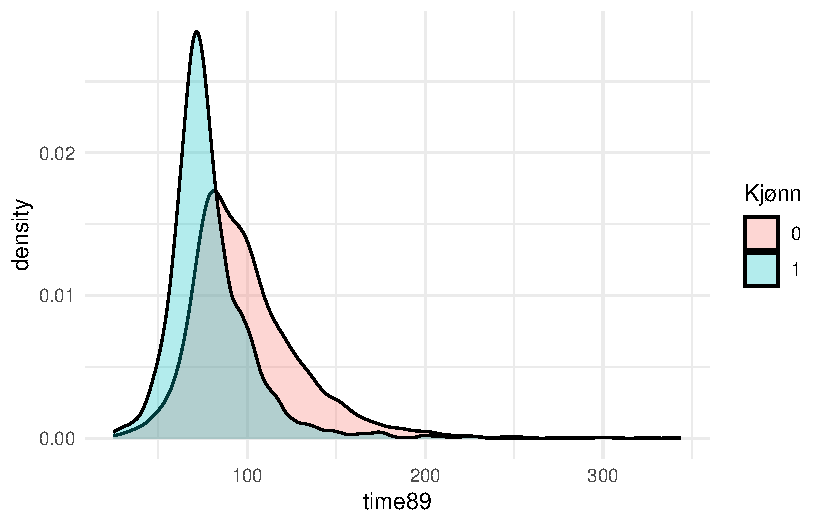
\includegraphics{./grafikk_files/figure-pdf/unnamed-chunk-13-1.pdf}

}

\end{figure}

\hypertarget{flere-variable-samtidig}{%
\subsection{Flere variable samtidig}\label{flere-variable-samtidig}}

\hypertarget{boksplot}{%
\subsubsection{Boksplot}\label{boksplot}}

\begin{Shaded}
\begin{Highlighting}[]
\FunctionTok{ggplot}\NormalTok{(abu89, }\FunctionTok{aes}\NormalTok{(}\AttributeTok{y =}\NormalTok{ time89, }\AttributeTok{group =}\NormalTok{ klasse89)) }\SpecialCharTok{+}
  \FunctionTok{geom\_boxplot}\NormalTok{()}\SpecialCharTok{+}
  \FunctionTok{theme\_minimal}\NormalTok{()}
\end{Highlighting}
\end{Shaded}

\begin{figure}[H]

{\centering 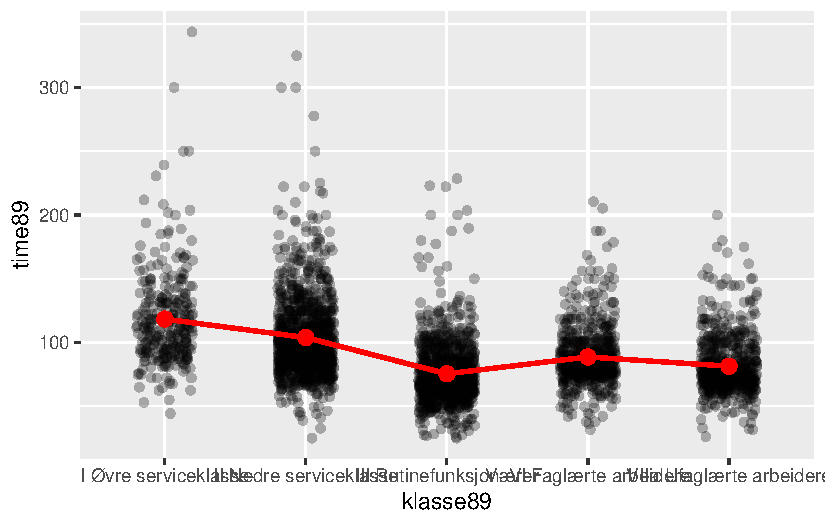
\includegraphics{./grafikk_files/figure-pdf/unnamed-chunk-14-1.pdf}

}

\end{figure}

\hypertarget{scatterplot}{%
\subsubsection{Scatterplot}\label{scatterplot}}

\begin{Shaded}
\begin{Highlighting}[]
\FunctionTok{ggplot}\NormalTok{(abu89, }\FunctionTok{aes}\NormalTok{(}\AttributeTok{x =}\NormalTok{ age, }\AttributeTok{y =}\NormalTok{ time89)) }\SpecialCharTok{+}
  \FunctionTok{geom\_point}\NormalTok{(}\AttributeTok{alpha=}\NormalTok{.}\DecValTok{3}\NormalTok{)}\SpecialCharTok{+}
  \FunctionTok{theme\_minimal}\NormalTok{()}
\end{Highlighting}
\end{Shaded}

\begin{figure}[H]

{\centering 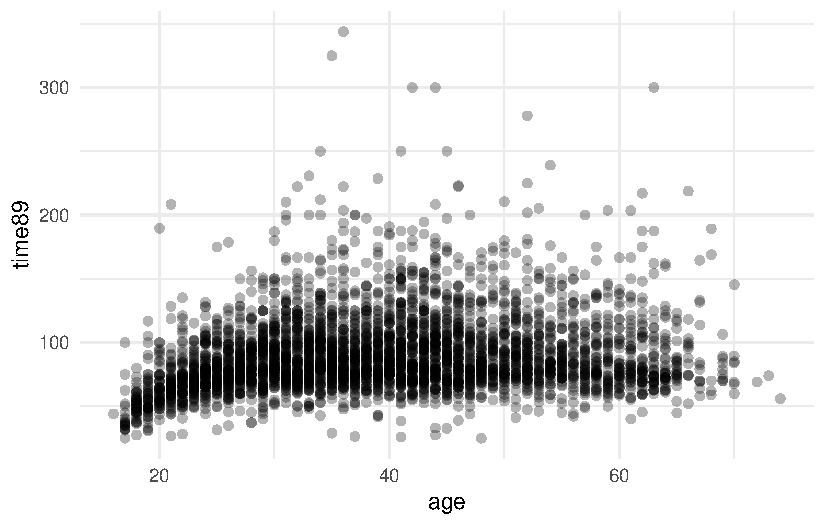
\includegraphics{./grafikk_files/figure-pdf/unnamed-chunk-15-1.pdf}

}

\end{figure}

\begin{Shaded}
\begin{Highlighting}[]
\FunctionTok{ggplot}\NormalTok{(abu89, }\FunctionTok{aes}\NormalTok{(}\AttributeTok{x =}\NormalTok{ age, }\AttributeTok{y =}\NormalTok{ time89)) }\SpecialCharTok{+}
  \FunctionTok{geom\_jitter}\NormalTok{(}\AttributeTok{alpha=}\NormalTok{.}\DecValTok{1}\NormalTok{, }\AttributeTok{width =}\NormalTok{ .}\DecValTok{3}\NormalTok{)}\SpecialCharTok{+}
  \FunctionTok{theme\_minimal}\NormalTok{()}
\end{Highlighting}
\end{Shaded}

\begin{figure}[H]

{\centering 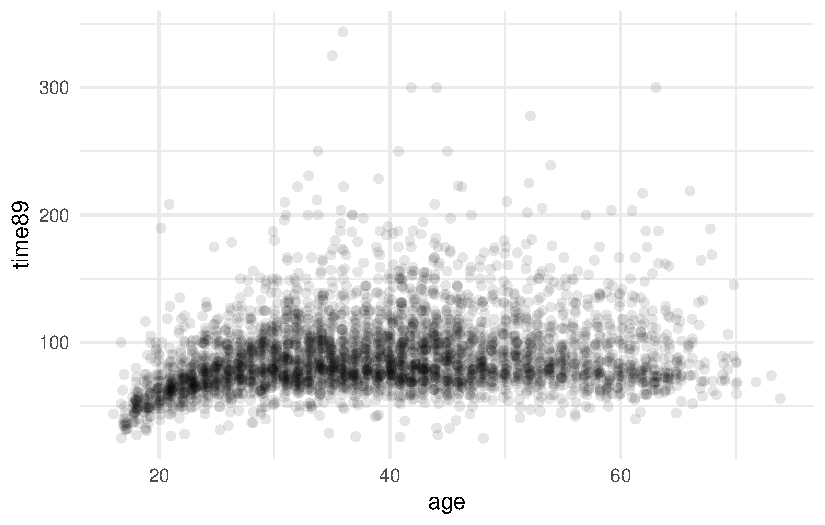
\includegraphics{./grafikk_files/figure-pdf/unnamed-chunk-16-1.pdf}

}

\end{figure}

\hypertarget{ridgeplot}{%
\subsubsection{Ridgeplot}\label{ridgeplot}}

Ridgeplot er en annen måte å sammenligne en kontinuerlig fordeling
betinget på en gruppering.

\begin{Shaded}
\begin{Highlighting}[]
\FunctionTok{library}\NormalTok{(ggridges)}
\FunctionTok{ggplot}\NormalTok{( abu89,  }\FunctionTok{aes}\NormalTok{(}\AttributeTok{y =}\NormalTok{ klasse89, }\AttributeTok{x =}\NormalTok{ time89)) }\SpecialCharTok{+}
  \FunctionTok{geom\_density\_ridges}\NormalTok{() }
\end{Highlighting}
\end{Shaded}

\begin{figure}[H]

{\centering 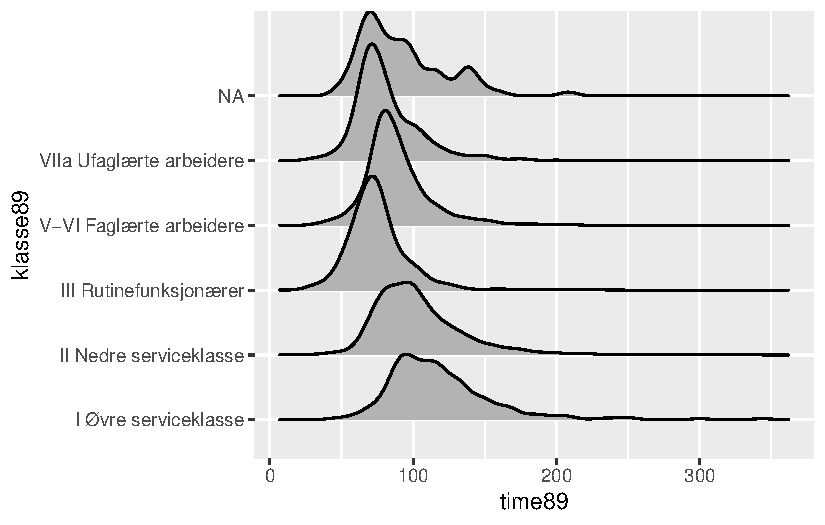
\includegraphics{./grafikk_files/figure-pdf/unnamed-chunk-17-1.pdf}

}

\end{figure}

\hypertarget{oppgaver-2}{%
\section{Oppgaver}\label{oppgaver-2}}

Slå opp i boken \href{https://r4ds.had.co.nz/data-visualisation.html}{R
for data science} hvis du står fast eller ikke skjønner hva koden betyr.

\leavevmode\vadjust pre{\hypertarget{exr-}{}}%
\begin{exercise}[]\label{exr-}

Last ned datasettet abu89 fra angitt hjemmeside og les inn dataene til R
som vist ovenfor. Lag den samme grafikken som vist her, gjør noen
endringer på kodene for å endre utseendet på plottene. Det er et mål at
du skal forstå hva hver enkelt kommando gjør.

\end{exercise}

\leavevmode\vadjust pre{\hypertarget{exr-}{}}%
\begin{exercise}[]\label{exr-}

Last inn datasettet NorLAG i R. Velg noen variable som du selv tenker
kan være informative å se nærmere på. Bruk de samme teknikkene på disse
variablene.

\end{exercise}

\hypertarget{deskriptive-tabeller}{%
\chapter{Deskriptive tabeller}\label{deskriptive-tabeller}}

\begin{Shaded}
\begin{Highlighting}[]
\FunctionTok{library}\NormalTok{(tidyverse)}
\FunctionTok{library}\NormalTok{(gtsummary)}
\end{Highlighting}
\end{Shaded}

Det kan være ulike grunner til å lage deskriptiv statistikk, og hva du
skal bruke tabellene til kan ha betydning for hvordan du lager dem. Noen
ganger skal du bare sjekke noen tall, og da er det ingen grunn til å
bruke tid på å gjøre tabellen spesiell pen. Andre ganger skal tabellen
publiseres i en rapport, på en nettside eller i en vitenskapelig
artikkel - eller mest aktuelt på kort sikt: i en masteroppgave. Da må
tabellene se ordentlige ut. Nedenfor skal vi se på begge mulighetene.

\hypertarget{quick-and-dirty-oppsummeringer}{%
\section{Quick-and-dirty
oppsummeringer}\label{quick-and-dirty-oppsummeringer}}

Først og fremst har vi funksjonen \texttt{summary()}. Når denne brukes
på et objekt vil hva slags output du får avhenge av objekttypen. Derfor
vil \texttt{summary()} gi forskjellig output om det er en vektor, et
datasett eller et regresjonsobjekt etc. Vi avgrenser oss til datasett
her.

Her er output for hele datasettet.

\begin{Shaded}
\begin{Highlighting}[]
\FunctionTok{summary}\NormalTok{(abu89)}
\end{Highlighting}
\end{Shaded}

\begin{verbatim}
     io_nr          time89             ed             age       
 Min.   :   3   Min.   : 25.00   Min.   : 0.00   Min.   :16.00  
 1st Qu.:1542   1st Qu.: 71.00   1st Qu.: 1.00   1st Qu.:30.00  
 Median :3093   Median : 83.33   Median : 3.00   Median :39.00  
 Mean   :3105   Mean   : 90.15   Mean   : 2.69   Mean   :39.65  
 3rd Qu.:4644   3rd Qu.:102.56   3rd Qu.: 3.00   3rd Qu.:48.00  
 Max.   :6258   Max.   :343.75   Max.   :11.00   Max.   :74.00  
                NA's   :368                                     
     female                           klasse89    promot          fexp       
 Min.   :0.0000   I Øvre serviceklasse    : 328   NEI:2568   Min.   :0.0000  
 1st Qu.:0.0000   II Nedre serviceklasse  :1181   JA :1559   1st Qu.:0.2000  
 Median :0.0000   III Rutinefunksjonærer  :1248              Median :0.7000  
 Mean   :0.4686   V-VI Faglærte arbeidere : 648              Mean   :0.9451  
 3rd Qu.:1.0000   VIIa Ufaglærte arbeidere: 637              3rd Qu.:1.4000  
 Max.   :1.0000   NA's                    :  85              Max.   :4.9000  
                                                                             
    private    
 Public :1602  
 Private:2525  
               
               
               
               
               
\end{verbatim}

Merk at \texttt{summary()} rapporterer forskjellig basert på om
variabelen er kontinuerlig eller kategorisk. For kontinuerlige variable
gis min/max, kvartiler, median og gjennomsnitt. For kategoriske variable
gis det antall i hver kategori. Hvis det er manglende verdier på en
variabel står det oppført nederst som antall
\texttt{NA\textquotesingle{}s}.

Merk her at variabelen female er definert som kontinuerlig selv om det
bare er to verdier. Det ville være mer hensiktsmessig å gjøre om denne
variabelen til kategorisk.

Man kan også bruke \texttt{summary()} på enkeltvariable med bruk av
\texttt{\$} som følger:

\begin{Shaded}
\begin{Highlighting}[]
\FunctionTok{summary}\NormalTok{(abu89}\SpecialCharTok{$}\NormalTok{time89)}
\end{Highlighting}
\end{Shaded}

\begin{verbatim}
   Min. 1st Qu.  Median    Mean 3rd Qu.    Max.    NA's 
  25.00   71.00   83.33   90.15  102.56  343.75     368 
\end{verbatim}

Da får man altså bare tallene for den variabelen man har angitt etter
dollartegnet.

\hypertarget{enkeltfunksjoner}{%
\subsection{Enkeltfunksjoner}\label{enkeltfunksjoner}}

Man kan hente ut hvert av disse tallene spesifikt fremfor å bruke
\texttt{summary()}. Det er egne funksjoner for dette, og de kan også
brukes når man gjør databearbeiding for litt andre formål. Vi ser her på
de viktigste.

Hva om man vil ha en kvartil som ikke er oppgitt i forvalget? Da kan man
bruke funksjonen \texttt{quantile()}. Argumentene i denne funksjonen er
hvilken variabel og hvilket prosentil. Som vi ovenfor inneholder time89
noen NA. Vi må i tillegg bestemme hva vi ønsker å gjøre med NA i
beregningen, og vi vil her se bort fra disse ved å angi
\texttt{na.rm\ =\ TRUE}. Ellers får man feilmelding.

Her er eksempel med første kvartil som skal gi samme svar som ovenfor:

\begin{Shaded}
\begin{Highlighting}[]
\FunctionTok{quantile}\NormalTok{(abu89}\SpecialCharTok{$}\NormalTok{time89, .}\DecValTok{25}\NormalTok{, }\AttributeTok{na.rm =} \ConstantTok{TRUE}\NormalTok{)}
\end{Highlighting}
\end{Shaded}

\begin{verbatim}
25% 
 71 
\end{verbatim}

Her er en variant der man ber om 95-prosentilen:

\begin{Shaded}
\begin{Highlighting}[]
\FunctionTok{quantile}\NormalTok{(abu89}\SpecialCharTok{$}\NormalTok{time89, .}\DecValTok{95}\NormalTok{, }\AttributeTok{na.rm =} \ConstantTok{TRUE}\NormalTok{)}
\end{Highlighting}
\end{Shaded}

\begin{verbatim}
     95% 
148.0362 
\end{verbatim}

Man kan også be om flere prosentiler. Da listes disse opp innenfor en
\texttt{c()} som følger. Her gis prosentilene for 5, 10, 90 og 95
prosent.

\begin{Shaded}
\begin{Highlighting}[]
\FunctionTok{quantile}\NormalTok{(abu89}\SpecialCharTok{$}\NormalTok{time89, }\FunctionTok{c}\NormalTok{(.}\DecValTok{05}\NormalTok{, .}\DecValTok{10}\NormalTok{, .}\DecValTok{90}\NormalTok{, .}\DecValTok{95}\NormalTok{), }\AttributeTok{na.rm =} \ConstantTok{TRUE}\NormalTok{)}
\end{Highlighting}
\end{Shaded}

\begin{verbatim}
       5%       10%       90%       95% 
 54.91651  61.00000 127.77778 148.03618 
\end{verbatim}

Gjennomsnittet av en variabel gis ved funksjonen \texttt{mean()}:

\begin{Shaded}
\begin{Highlighting}[]
\FunctionTok{mean}\NormalTok{(abu89}\SpecialCharTok{$}\NormalTok{time89, }\AttributeTok{na.rm =} \ConstantTok{TRUE}\NormalTok{)}
\end{Highlighting}
\end{Shaded}

\begin{verbatim}
[1] 90.14948
\end{verbatim}

Standardavviket gis ved \texttt{sd()}:

\begin{Shaded}
\begin{Highlighting}[]
\FunctionTok{sd}\NormalTok{(abu89}\SpecialCharTok{$}\NormalTok{time89, }\AttributeTok{na.rm =} \ConstantTok{TRUE}\NormalTok{)}
\end{Highlighting}
\end{Shaded}

\begin{verbatim}
[1] 30.31473
\end{verbatim}

Medianen kan angis med \texttt{quantile()}, men enklere med
\texttt{median()}:

\begin{Shaded}
\begin{Highlighting}[]
\FunctionTok{median}\NormalTok{(abu89}\SpecialCharTok{$}\NormalTok{time89, }\AttributeTok{na.rm =} \ConstantTok{TRUE}\NormalTok{)}
\end{Highlighting}
\end{Shaded}

\begin{verbatim}
[1] 83.33333
\end{verbatim}

Vi trenger også ofte antall. \texttt{nrow()} gir antall rader, dvs.
antall observasjoner i datasettet

\begin{Shaded}
\begin{Highlighting}[]
\FunctionTok{nrow}\NormalTok{(abu89)}
\end{Highlighting}
\end{Shaded}

\begin{verbatim}
[1] 4127
\end{verbatim}

Tilsvarende gir \texttt{ncol()} antall kolonner, mens \texttt{dim()} gir
begge deler:

\begin{Shaded}
\begin{Highlighting}[]
\FunctionTok{ncol}\NormalTok{(abu89)}
\end{Highlighting}
\end{Shaded}

\begin{verbatim}
[1] 9
\end{verbatim}

\begin{Shaded}
\begin{Highlighting}[]
\FunctionTok{dim}\NormalTok{(abu89)}
\end{Highlighting}
\end{Shaded}

\begin{verbatim}
[1] 4127    9
\end{verbatim}

\hypertarget{professjonelle-tabeller-med-gtsummary}{%
\section{Professjonelle tabeller med
gtsummary}\label{professjonelle-tabeller-med-gtsummary}}

For å lage ordentlig professjonelle tabeller kreves det mer. For det
første skal de se ordentlige ut, men de skal også kunne eksporteres til
andre formater på en hensiktsmessig måte.

I R finnes det en hel rekke slike funksjoner. Her har vi vektlagt pakken
\texttt{gtsummary} fordi den gir gode tabeller fra helt enkle til ganske
avanserte relativt lett. Det er også mange muligheter for å justere
tabellene slik du vil. Dessuten kan resultatene eksporteres lett til de
fleste aktuelle formater (Word, html, pdf, Excel, latex).

Avanserte brukere vil muligens se begrensningene i denne pakken og
foretrekke noe annet. De fleste vil kunne lage det aller meste med denne
pakken.

Vi starter med en enkel oversiktstabell med alle variablene i
datasettet. Men vi fjerner løpenummeret for person, nemlig variabelen
\emph{io\_nr} fordi den ikke inneholder noe analyserbar informasjon.

\begin{Shaded}
\begin{Highlighting}[]
\NormalTok{abu89 }\SpecialCharTok{\%\textgreater{}\%} 
  \FunctionTok{select}\NormalTok{(}\SpecialCharTok{{-}}\NormalTok{io\_nr) }\SpecialCharTok{\%\textgreater{}\%} 
  \FunctionTok{tbl\_summary}\NormalTok{()}
\end{Highlighting}
\end{Shaded}

\begin{verbatim}
Table printed with `knitr::kable()`, not {gt}. Learn why at
https://www.danieldsjoberg.com/gtsummary/articles/rmarkdown.html
To suppress this message, include `message = FALSE` in code chunk header.
\end{verbatim}

\begin{longtable}[]{@{}lc@{}}
\toprule()
\textbf{Characteristic} & \textbf{N = 4,127} \\
\midrule()
\endhead
Gjennomsnittlig timelønn 1989 & 83 (71, 103) \\
Unknown & 368 \\
År utdanning & \\
0 & 839 (20\%) \\
1 & 1,156 (28\%) \\
3 & 1,121 (27\%) \\
5 & 483 (12\%) \\
7 & 308 (7.5\%) \\
9 & 205 (5.0\%) \\
11 & 15 (0.4\%) \\
Alder & 39 (30, 48) \\
Respondentens kjønn & 1,934 (47\%) \\
Goldthorpe klasse 1989 & \\
I Øvre serviceklasse & 328 (8.1\%) \\
II Nedre serviceklasse & 1,181 (29\%) \\
III Rutinefunksjonærer & 1,248 (31\%) \\
V-VI Faglærte arbeidere & 648 (16\%) \\
VIIa Ufaglærte arbeidere & 637 (16\%) \\
Unknown & 85 \\
Noen gang forfremmet & \\
NEI & 2,568 (62\%) \\
JA & 1,559 (38\%) \\
Bedriftserfaring & 0.70 (0.20, 1.40) \\
Privat sektor & \\
Public & 1,602 (39\%) \\
Private & 2,525 (61\%) \\
\bottomrule()
\end{longtable}

Legg merke til at \texttt{tbl\_summary} gjør en del ting automatisk.
Først og fremst er bruker den \emph{variabel label} og \emph{factor
levels} i sidespalten. Ofte vil ikke variable ha slike labler, og da vil
det vises variabelnavnene. Variabelen \emph{kjønn} har ikke angitt
factor levels, og variabelen har bare verdiene 0 og 1, og da rapporteres
kun den ene kategorien (dvs. verdien 1). Vi kan legge til annen tekst
hvis vi ønsker.

Dernest er det en forhåndsinnstilling som angir at det for kontinuerlige
variable skal rapporteres median og interquartile range (IQR), dvs.
nedre og øvre kvartil i parentes. Det gir en god beskrivelse av
variablene, men vi skal endre dette nedenfor. For kategoriske variable
rapporteres det antall observasjoner og andelen i prosent i parentes.

Men merk at for antall år utdanning og kjønn, så er det rapportert som
kategoriske variable selv om variabeltypen er kontinuerlig.
\texttt{tbl\_summary} gjør dette fordi det er relativt få kategorier
slik at median og IQR ikke er så interessant uansett.

La oss først endre slik at det rapporteres gjennomsnitt og standardavvik
i stedet. Det er mer vanlig å gjøre selv om det ikke er noen regel for
dette. Funksjonen \texttt{theme\_gtsummary\_mean\_sd()} endrer
standardvalget for \texttt{tbl\_summary} i \emph{alle etterfølgende
tabeller}. Dermed slipper du endre neste gang. Flere themes finner du på
\href{https://www.danieldsjoberg.com/gtsummary/articles/themes.html}{pakkens
hjemmeside}. For å gå tilbake til opprinnelig theme brukes funksjonen
\texttt{reset\_gtsummary\_theme()}.

Vi kan endre andre ting ved tabellen med noen enkle grep. Alle variable
kan endre navn i forspalten med å legge til argumentet
\texttt{label\ =}. Nedenfor er to variable endret for å vise hvordan man
endrer flere variable. Når det er flere variable må de spesifiseres
innenfor argumentet \texttt{list()} som nedenfor. Her endrer vi også
label for variabelen female og klasse89.

Noen ganger kan man også ønske å endre hvordan en variabel presenteres.
Et vanlig behov er å presisere hvilken type en variabel er. I dette
tilfellet er utdanning antall år etter obligatorisk skolenivå, så det er
egentlig en kontinuerlig variabel selv om antall verdier er få. Vi kan
velge å presisere at denne er av typen \emph{continuous}. Nedenfor
presiserer vi også at female er kategorisk, \emph{dichotomous}, selv om
denne ble presentert riktig uansett. Vi bruker argumentet
\texttt{type\ =} og flere variable må oppgis innenfor \texttt{list()}.

En siste ting vi kan endre er å ikke rapportere NA. Det er ikke oppgitt
timelønn for alle, så antall NA er rapportert for seg. Det kan være
fint, men kan også hende vi ikke ønsker det. Nedenfor er det derfor også
lagt til \texttt{missing\ =\ "no"}.

\begin{Shaded}
\begin{Highlighting}[]
\FunctionTok{theme\_gtsummary\_mean\_sd}\NormalTok{()}
\NormalTok{abu89 }\SpecialCharTok{\%\textgreater{}\%} 
  \FunctionTok{select}\NormalTok{(}\SpecialCharTok{{-}}\NormalTok{io\_nr) }\SpecialCharTok{\%\textgreater{}\%} 
  \FunctionTok{tbl\_summary}\NormalTok{(}\AttributeTok{label =} \FunctionTok{list}\NormalTok{(female }\SpecialCharTok{\textasciitilde{}} \StringTok{"Kjønn"}\NormalTok{, }\AttributeTok{klasse89 =} \StringTok{"Klasse"}\NormalTok{), }
              \AttributeTok{type =} \FunctionTok{list}\NormalTok{(ed }\SpecialCharTok{\textasciitilde{}} \StringTok{"continuous"}\NormalTok{, female }\SpecialCharTok{\textasciitilde{}} \StringTok{"dichotomous"}\NormalTok{), }
              \AttributeTok{missing =} \StringTok{"no"}\NormalTok{)}
\end{Highlighting}
\end{Shaded}

\begin{verbatim}
Table printed with `knitr::kable()`, not {gt}. Learn why at
https://www.danieldsjoberg.com/gtsummary/articles/rmarkdown.html
To suppress this message, include `message = FALSE` in code chunk header.
\end{verbatim}

\begin{longtable}[]{@{}lc@{}}
\toprule()
\textbf{Characteristic} & \textbf{N = 4,127} \\
\midrule()
\endhead
Gjennomsnittlig timelønn 1989 & 90 (30) \\
År utdanning & 2.69 (2.56) \\
Alder & 40 (12) \\
Kjønn & 1,934 (47\%) \\
Klasse & \\
I Øvre serviceklasse & 328 (8.1\%) \\
II Nedre serviceklasse & 1,181 (29\%) \\
III Rutinefunksjonærer & 1,248 (31\%) \\
V-VI Faglærte arbeidere & 648 (16\%) \\
VIIa Ufaglærte arbeidere & 637 (16\%) \\
Noen gang forfremmet & \\
NEI & 2,568 (62\%) \\
JA & 1,559 (38\%) \\
Bedriftserfaring & 0.95 (0.91) \\
Privat sektor & \\
Public & 1,602 (39\%) \\
Private & 2,525 (61\%) \\
\bottomrule()
\end{longtable}

Ofte vil vi ha en tabell som ikke bare viser univariat fordeling, men
bi-variate, altså fordelt på to eller flere grupper. Det er f.eks.
ganske vanlig å vise tabeller fordelt på kjønn. Det kan vi også gjøre
her ved å legge til argumentet \texttt{by\ =\ female}. Nedenfor er det
også forenklet argumentene for \texttt{label\ =} og \texttt{type\ =}. I
slike tilfeller vil vi ofte ha totalen i tillegg til per gruppe, og det
gjør vi ved å legge til funksjonen \texttt{add\_overall()}.

For de kontinuerlige variablene får vi ikke antallet som inngår i
beregningene. Vi vil gjerne vise antall ikke-missing verdier - særlig
fordi vi tok vekk NA som egen rad ovenfor. Dette gjør vi ved å legge til
funksjonen \texttt{add\_n()}.

\begin{Shaded}
\begin{Highlighting}[]
\NormalTok{abu89 }\SpecialCharTok{\%\textgreater{}\%} 
  \FunctionTok{select}\NormalTok{(}\SpecialCharTok{{-}}\NormalTok{io\_nr) }\SpecialCharTok{\%\textgreater{}\%} 
  \FunctionTok{mutate}\NormalTok{(}\AttributeTok{female =} \FunctionTok{ifelse}\NormalTok{(female }\SpecialCharTok{==} \DecValTok{0}\NormalTok{, }\StringTok{"Menn"}\NormalTok{, }\StringTok{"Kvinner"}\NormalTok{)) }\SpecialCharTok{\%\textgreater{}\%} 
    \FunctionTok{tbl\_summary}\NormalTok{(}\AttributeTok{by =}\NormalTok{ female, }
                \AttributeTok{label =} \FunctionTok{list}\NormalTok{(}\AttributeTok{klasse89 =} \StringTok{"Klasse"}\NormalTok{), }
              \AttributeTok{type =} \FunctionTok{list}\NormalTok{(ed }\SpecialCharTok{\textasciitilde{}} \StringTok{"continuous"}\NormalTok{), }
              \AttributeTok{missing =} \StringTok{"no"}\NormalTok{) }\SpecialCharTok{\%\textgreater{}\%} 
  \FunctionTok{add\_overall}\NormalTok{() }\SpecialCharTok{\%\textgreater{}\%} 
  \FunctionTok{add\_n}\NormalTok{()}
\end{Highlighting}
\end{Shaded}

\begin{verbatim}
Table printed with `knitr::kable()`, not {gt}. Learn why at
https://www.danieldsjoberg.com/gtsummary/articles/rmarkdown.html
To suppress this message, include `message = FALSE` in code chunk header.
\end{verbatim}

\begin{longtable}[]{@{}
  >{\raggedright\arraybackslash}p{(\columnwidth - 8\tabcolsep) * \real{0.2830}}
  >{\centering\arraybackslash}p{(\columnwidth - 8\tabcolsep) * \real{0.0660}}
  >{\centering\arraybackslash}p{(\columnwidth - 8\tabcolsep) * \real{0.2264}}
  >{\centering\arraybackslash}p{(\columnwidth - 8\tabcolsep) * \real{0.2264}}
  >{\centering\arraybackslash}p{(\columnwidth - 8\tabcolsep) * \real{0.1981}}@{}}
\toprule()
\begin{minipage}[b]{\linewidth}\raggedright
\textbf{Characteristic}
\end{minipage} & \begin{minipage}[b]{\linewidth}\centering
\textbf{N}
\end{minipage} & \begin{minipage}[b]{\linewidth}\centering
\textbf{Overall}, N = 4,127
\end{minipage} & \begin{minipage}[b]{\linewidth}\centering
\textbf{Kvinner}, N = 1,934
\end{minipage} & \begin{minipage}[b]{\linewidth}\centering
\textbf{Menn}, N = 2,193
\end{minipage} \\
\midrule()
\endhead
Gjennomsnittlig timelønn 1989 & 3,759 & 90 (30) & 79 (24) & 100 (32) \\
År utdanning & 4,127 & 2.69 (2.56) & 2.38 (2.40) & 2.96 (2.66) \\
Alder & 4,127 & 40 (12) & 40 (13) & 40 (12) \\
Klasse & 4,042 & & & \\
I Øvre serviceklasse & & 328 (8.1\%) & 74 (3.9\%) & 254 (12\%) \\
II Nedre serviceklasse & & 1,181 (29\%) & 555 (29\%) & 626 (29\%) \\
III Rutinefunksjonærer & & 1,248 (31\%) & 986 (52\%) & 262 (12\%) \\
V-VI Faglærte arbeidere & & 648 (16\%) & 46 (2.4\%) & 602 (28\%) \\
VIIa Ufaglærte arbeidere & & 637 (16\%) & 244 (13\%) & 393 (18\%) \\
Noen gang forfremmet & 4,127 & & & \\
NEI & & 2,568 (62\%) & 1,308 (68\%) & 1,260 (57\%) \\
JA & & 1,559 (38\%) & 626 (32\%) & 933 (43\%) \\
Bedriftserfaring & 4,127 & 0.95 (0.91) & 0.83 (0.81) & 1.05 (0.97) \\
Privat sektor & 4,127 & & & \\
Public & & 1,602 (39\%) & 1,016 (53\%) & 586 (27\%) \\
Private & & 2,525 (61\%) & 918 (47\%) & 1,607 (73\%) \\
\bottomrule()
\end{longtable}

Men vi kan lage mer kompliserte tabeller også. La oss si at vi ønsker å
lage den samme tabellen som over, men fordelt på to grupper. Det kan
være relevant å sammenligne offentlig og privat sektor. En mulighet er å
lage en ny grupperingsvariabel ved å slå sammen kjønn og sektor slik at
vi får fire kategorier. Men vi får et bedre resultat ved å lage en
stratifisert tabell med funksjonen \texttt{tbl\_strata()}. Det er litt
kryptisk syntaks, men det viktige er å angi hvilken variabel det skal
stratifiseres etter med argumentet \texttt{strata\ =} etterfulgt av
\texttt{.tbl\_fun\ =\ \textasciitilde{}\ .x\ \%\textgreater{}\%}, så
kommer \texttt{tble\_summary} etter dette. Her er det også lagt til en
ekstra header med antall observasjoner.

\begin{Shaded}
\begin{Highlighting}[]
\NormalTok{abu89 }\SpecialCharTok{\%\textgreater{}\%} 
  \FunctionTok{select}\NormalTok{(}\SpecialCharTok{{-}}\NormalTok{io\_nr) }\SpecialCharTok{\%\textgreater{}\%} 
  \FunctionTok{mutate}\NormalTok{(}\AttributeTok{female =} \FunctionTok{ifelse}\NormalTok{(female }\SpecialCharTok{==} \DecValTok{0}\NormalTok{, }\StringTok{"Menn"}\NormalTok{, }\StringTok{"Kvinner"}\NormalTok{)) }\SpecialCharTok{\%\textgreater{}\%} 
  \FunctionTok{tbl\_strata}\NormalTok{(}\AttributeTok{strata =}\NormalTok{ private, }
             \AttributeTok{.tbl\_fun =} 
               \SpecialCharTok{\textasciitilde{}}\NormalTok{ .x }\SpecialCharTok{\%\textgreater{}\%}
               \FunctionTok{tbl\_summary}\NormalTok{(}\AttributeTok{by =}\NormalTok{ female, }
              \AttributeTok{label =} \FunctionTok{list}\NormalTok{(}\AttributeTok{klasse89 =} \StringTok{"Klasse"}\NormalTok{), }
              \AttributeTok{type =} \FunctionTok{list}\NormalTok{(ed }\SpecialCharTok{\textasciitilde{}} \StringTok{"continuous"}\NormalTok{), }
              \AttributeTok{missing =} \StringTok{"no"}\NormalTok{) }\SpecialCharTok{\%\textgreater{}\%}
               \FunctionTok{add\_n}\NormalTok{(),}
    \AttributeTok{.header =} \StringTok{"**\{strata\}**, N = \{n\}"}
\NormalTok{    )}
\end{Highlighting}
\end{Shaded}

\begin{verbatim}
Table printed with `knitr::kable()`, not {gt}. Learn why at
https://www.danieldsjoberg.com/gtsummary/articles/rmarkdown.html
To suppress this message, include `message = FALSE` in code chunk header.
\end{verbatim}

\begin{longtable}[]{@{}
  >{\raggedright\arraybackslash}p{(\columnwidth - 12\tabcolsep) * \real{0.2308}}
  >{\centering\arraybackslash}p{(\columnwidth - 12\tabcolsep) * \real{0.0538}}
  >{\centering\arraybackslash}p{(\columnwidth - 12\tabcolsep) * \real{0.1846}}
  >{\centering\arraybackslash}p{(\columnwidth - 12\tabcolsep) * \real{0.1462}}
  >{\centering\arraybackslash}p{(\columnwidth - 12\tabcolsep) * \real{0.0538}}
  >{\centering\arraybackslash}p{(\columnwidth - 12\tabcolsep) * \real{0.1692}}
  >{\centering\arraybackslash}p{(\columnwidth - 12\tabcolsep) * \real{0.1615}}@{}}
\toprule()
\begin{minipage}[b]{\linewidth}\raggedright
\textbf{Characteristic}
\end{minipage} & \begin{minipage}[b]{\linewidth}\centering
\textbf{N}
\end{minipage} & \begin{minipage}[b]{\linewidth}\centering
\textbf{Kvinner}, N = 1,016
\end{minipage} & \begin{minipage}[b]{\linewidth}\centering
\textbf{Menn}, N = 586
\end{minipage} & \begin{minipage}[b]{\linewidth}\centering
\textbf{N}
\end{minipage} & \begin{minipage}[b]{\linewidth}\centering
\textbf{Kvinner}, N = 918
\end{minipage} & \begin{minipage}[b]{\linewidth}\centering
\textbf{Menn}, N = 1,607
\end{minipage} \\
\midrule()
\endhead
Gjennomsnittlig timelønn 1989 & 1,403 & 82 (23) & 100 (28) & 2,356 & 76
(24) & 100 (33) \\
År utdanning & 1,602 & 2.88 (2.67) & 4.22 (3.12) & 2,525 & 1.82 (1.92) &
2.50 (2.31) \\
Alder & 1,602 & 42 (12) & 43 (11) & 2,525 & 37 (13) & 39 (12) \\
Klasse & 1,592 & & & 2,450 & & \\
I Øvre serviceklasse & & 55 (5.4\%) & 150 (26\%) & & 19 (2.1\%) & 104
(6.7\%) \\
II Nedre serviceklasse & & 340 (34\%) & 196 (34\%) & & 215 (24\%) & 430
(28\%) \\
III Rutinefunksjonærer & & 507 (50\%) & 64 (11\%) & & 479 (54\%) & 198
(13\%) \\
V-VI Faglærte arbeidere & & 5 (0.5\%) & 114 (20\%) & & 41 (4.6\%) & 488
(31\%) \\
VIIa Ufaglærte arbeidere & & 104 (10\%) & 57 (9.8\%) & & 140 (16\%) &
336 (22\%) \\
Noen gang forfremmet & 1,602 & & & 2,525 & & \\
NEI & & 696 (69\%) & 318 (54\%) & & 612 (67\%) & 942 (59\%) \\
JA & & 320 (31\%) & 268 (46\%) & & 306 (33\%) & 665 (41\%) \\
Bedriftserfaring & 1,602 & 0.93 (0.85) & 1.15 (0.94) & 2,525 & 0.72
(0.74) & 1.01 (0.98) \\
\bottomrule()
\end{longtable}

Det går også an å lage langt mer avanserte tabeller enn dette, og alle
deler kan modifiseres. Men vi går ikke inn på dette her. Ved behov
finner du instruksjoner på
\href{https://www.danieldsjoberg.com/gtsummary/index.html}{pakkens
hjemmeside}.

\hypertarget{eksport-av-tabeller}{%
\subsection{Eksport av tabeller}\label{eksport-av-tabeller}}

Du skal aldri bruke ``klipp og lim'' for å få en tabell over i et
tekstbehandlingsprogram. Trikset er å konvertere tabellen til gt-format
som har en eksportfunksjon til MS Word.

Først lagres tabellen i et eget objekt.

\begin{Shaded}
\begin{Highlighting}[]
\NormalTok{fintabell }\OtherTok{\textless{}{-}}\NormalTok{ abu89 }\SpecialCharTok{\%\textgreater{}\%} 
  \FunctionTok{select}\NormalTok{(}\SpecialCharTok{{-}}\NormalTok{io\_nr) }\SpecialCharTok{\%\textgreater{}\%} 
  \FunctionTok{mutate}\NormalTok{(}\AttributeTok{female =} \FunctionTok{ifelse}\NormalTok{(female }\SpecialCharTok{==} \DecValTok{0}\NormalTok{, }\StringTok{"Menn"}\NormalTok{, }\StringTok{"Kvinner"}\NormalTok{)) }\SpecialCharTok{\%\textgreater{}\%} 
  \FunctionTok{tbl\_strata}\NormalTok{(}\AttributeTok{strata =}\NormalTok{ private, }
             \AttributeTok{.tbl\_fun =} 
               \SpecialCharTok{\textasciitilde{}}\NormalTok{ .x }\SpecialCharTok{\%\textgreater{}\%}
               \FunctionTok{tbl\_summary}\NormalTok{(}\AttributeTok{by =}\NormalTok{ female, }
              \AttributeTok{label =} \FunctionTok{list}\NormalTok{(}\AttributeTok{klasse89 =} \StringTok{"Klasse"}\NormalTok{), }
              \AttributeTok{type =} \FunctionTok{list}\NormalTok{(ed }\SpecialCharTok{\textasciitilde{}} \StringTok{"continuous"}\NormalTok{), }
              \AttributeTok{missing =} \StringTok{"no"}\NormalTok{) }\SpecialCharTok{\%\textgreater{}\%}
               \FunctionTok{add\_n}\NormalTok{(),}
    \AttributeTok{.header =} \StringTok{"**\{strata\}**, N = \{n\}"}
\NormalTok{    )}
\end{Highlighting}
\end{Shaded}

Så kan tabellen eksporteres til Word, og evt. redigeres videre der hvis
det trengs. På dette nivået kan det være mer tidsbesparende å gjøre
siste justeringer i Word fremfor å lære alle triks for å lage tabellen
fiks ferdig i R. (Skal du lage mange tabeller kan det likevel lønne seg
å gjøre mest mulig i R).

\begin{Shaded}
\begin{Highlighting}[]
\NormalTok{fintabell }\SpecialCharTok{\%\textgreater{}\%} 
  \FunctionTok{as\_gt}\NormalTok{() }\SpecialCharTok{\%\textgreater{}\%} 
\NormalTok{  gt}\SpecialCharTok{::}\FunctionTok{gtsave}\NormalTok{(}\AttributeTok{filename =} \StringTok{"output/fintabell.docx"}\NormalTok{)}
\end{Highlighting}
\end{Shaded}

Merk at eksport til docx-formatet krever at du har en relativt ny
installasjon av pakkene \{gt\} og \{gtsummary\}. Filhalen ``.docx''
innebærer at filen lagres i dette formatet. Tilsvarende kan du lagre i
.html, .pdf, .rtf, .png, .tex eller .ltex bare ved å endre filhalen.

En tilsvarende variant som noen av dere har lært på sosgeo1120 er å
bruke \texttt{as\_flextable} og en tilsvarende eksportfunksjon. Det er
selvsagt også helt ok. En tidligere versjon av \{gt\} kunne som sagt
ikke eksportere til Word, så da var \{flextable\} beste løsning. Men
pakken \{flextable\} har vist seg å være litt trøblete å installere på
noen pc'er, så da er det bedre å bruke \{gt\}.

\hypertarget{manuelle-tabeller}{%
\section{Manuelle tabeller}\label{manuelle-tabeller}}

Noen ganger trenger man å lage ganske spesifikke ting.

\hypertarget{for-datasettet-totalt}{%
\subsection{For datasettet totalt}\label{for-datasettet-totalt}}

\hypertarget{grupperte-statistikker}{%
\subsection{Grupperte statistikker}\label{grupperte-statistikker}}

\hypertarget{oppgaver-3}{%
\section{Oppgaver}\label{oppgaver-3}}

Slå opp i boken \href{https://r4ds.had.co.nz/data-visualisation.html}{R
for data science} hvis du står fast eller ikke skjønner hva koden betyr.

\leavevmode\vadjust pre{\hypertarget{exr-}{}}%
\begin{exercise}[]\label{exr-}

Bruk datasettet abu89 og lag de samme tabellene som vist her, gjør noen
endringer på kodene for å endre utseendet på tabellene. Det er et mål at
du skal forstå hva hver enkelt kommando gjør.

\end{exercise}

\leavevmode\vadjust pre{\hypertarget{exr-}{}}%
\begin{exercise}[]\label{exr-}

Last inn datasettet NorLAG i R. Velg noen variable som du selv tenker
kan være informative å se nærmere på. Bruk de samme teknikkene på disse
variablene.

\end{exercise}

\part{Del 3: Flere variable på en gang}

\hypertarget{regresjon-sammenheng-mellom-variable}{%
\chapter{Regresjon: Sammenheng mellom
variable}\label{regresjon-sammenheng-mellom-variable}}

\begin{Shaded}
\begin{Highlighting}[]
\FunctionTok{library}\NormalTok{(tidyverse)}
\FunctionTok{library}\NormalTok{(gtsummary)}
\end{Highlighting}
\end{Shaded}

Vi skal her se på helt grunnleggende lineær regresjon med en og to
forklaringsvariable.

\hypertarget{scatterplot-1}{%
\section{Scatterplot}\label{scatterplot-1}}

Bivariat regresjon beskriver sammenhengen mellom to variable. En
naturlig start er å se på et scatterplot. Her er en figur som viser
hvordan timelønn varierer med alder. I det nedenforstående er det brukt
jitter og gjennomsiktig farge for å håndtere overplotting.

I tillegg er det tegnet inn en linje som illustrerer \emph{trenden i
gjennomsnittlig lønn} med alder. Denne linjen skrår svakt oppover, som
altså betyr at gjennomsnittlig lønn øker noe med alder. Vi ser med det
blotte øyet at en rett linje ikke beskriver denne sammenhengen perfekt.
Først og fremst er det en stor variasjon rundt denne linjen, så det er
mye annet som påvirker lønna enn alder. Det er også verd å legge merke
til at i de yngste aldersgruppene er lønna en god del lavere - og
kanskje litt lavere i eldste aldersgrupper også. Så en rett linje er
kanskje ikke optimalt i utgangspunktet. Fordelen med en rett linje er at
vi kan si noe slikt som at ``gjennosmsnittslønna øker med x antall
kroner for hvert år eldre man blir''. Hvis linja er kurvlineær blir det
litt mer komplisert. Så et første poeng er at en slik linje er en
\emph{forenkling}, og det er en tilsiktet forenkling.

\begin{Shaded}
\begin{Highlighting}[]
\FunctionTok{ggplot}\NormalTok{(abu89, }\FunctionTok{aes}\NormalTok{(}\AttributeTok{x =}\NormalTok{age, }\AttributeTok{y =}\NormalTok{ time89))}\SpecialCharTok{+}
  \FunctionTok{geom\_jitter}\NormalTok{(}\AttributeTok{alpha =}\NormalTok{ .}\DecValTok{2}\NormalTok{)}\SpecialCharTok{+}
  \FunctionTok{geom\_smooth}\NormalTok{(}\AttributeTok{method =} \StringTok{"lm"}\NormalTok{, }\AttributeTok{se =} \ConstantTok{FALSE}\NormalTok{)}
\end{Highlighting}
\end{Shaded}

\begin{figure}[H]

{\centering \includegraphics{./linearRegresjon_files/figure-pdf/unnamed-chunk-4-1.pdf}

}

\end{figure}

Det er en viss tendens til at lønnen øker med alder, men det er ikke
helt lett å si hvor mye. Poenget med lineær regresjon er å beskrive en
gjennomsnittlig trend.

\begin{Shaded}
\begin{Highlighting}[]
\FunctionTok{ggplot}\NormalTok{(abu89, }\FunctionTok{aes}\NormalTok{(}\AttributeTok{x =}\NormalTok{age, }\AttributeTok{y =}\NormalTok{ time89))}\SpecialCharTok{+}
  \FunctionTok{geom\_jitter}\NormalTok{(}\AttributeTok{alpha =}\NormalTok{ .}\DecValTok{2}\NormalTok{)}\SpecialCharTok{+}
  \FunctionTok{geom\_smooth}\NormalTok{(}\AttributeTok{method =} \StringTok{"lm"}\NormalTok{, }\AttributeTok{se =} \ConstantTok{FALSE}\NormalTok{)}
\end{Highlighting}
\end{Shaded}

\begin{figure}[H]

{\centering 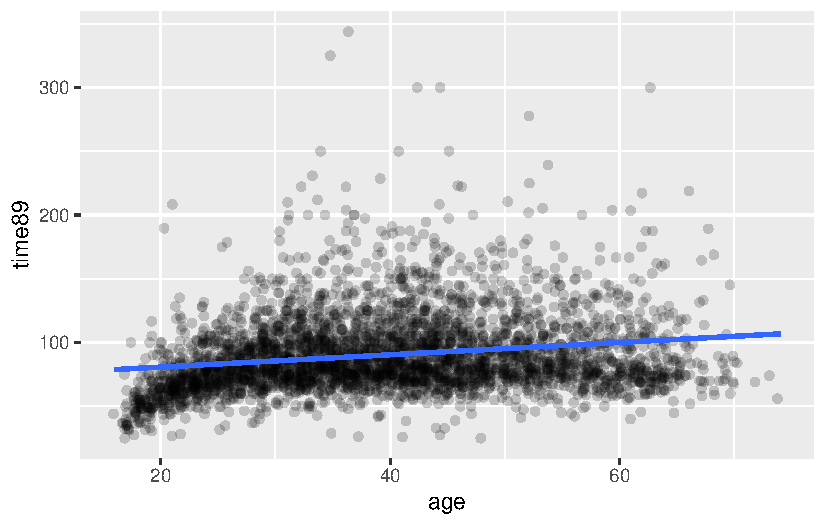
\includegraphics{./linearRegresjon_files/figure-pdf/unnamed-chunk-5-1.pdf}

}

\end{figure}

Denne trendlinja er hva vi vanligvis kaller regresjonslinje.

\hypertarget{regresjonslinja}{%
\section{Regresjonslinja}\label{regresjonslinja}}

Regresjonslinja kan beskrives med et \emph{stigningstall}, som sier hvor
bratt linjen er. Substansielt sett betyr det hvor mye utfallsvariabelen
(y-aksen) endres med økning i forklaringsvariabelen (x-aksen). I tillegg
trenger vi også vite hvor høyt/lavt linjen ligger.\footnote{Du kan jo
  tenke deg flere parallelle linjer i plottet ovenfor med samme
  stigningstall} Til det bruker vi startpunktet for linjen, der hvor
\(x\) har verdien 0. Dette må regnes ut, og det er akkurat dette
estimering av lineær regresjon gir oss.

Utregningen av regresjonslinja går vi ikke inn på her, men intuitivt
sett ønsker vi jo \emph{den beste linja} og ikke en hvilken som helst
omtrentlig linje. Datapunktene (de svarte punktene i grafen) er spredt
rundt linja, og avstanden mellom linje og punkt kalles
\emph{residualer}. Summen av disse residualene er grunnlaget for mål på
hvor godt regresjonslinja beskriver de faktiske dataene. Den beste linja
er definert som den som minimerer residualene. Det er dette som kalles
``minste kvadraters metode''.

I R estimeres regresjonsmodeller med funksjonen \texttt{lm}. Første
argument er en formel på formen
\texttt{utfallsvariabel\ \textasciitilde{}\ forklaringsvariabel}.
Rekkefølgen variablene oppgis i er altså viktig. Dernest må det
spesifiseres hvilket datasett som skal brukes med \texttt{data\ =}
.\footnote{Grunnen til det siste er at R kan ha flere datasett oppe
  samtidig, så R vet ikke nødvendigvis hvilket datasett du tenker på}

Legg alltid resultatene i et eget objekt med et navnt som er rimelig
enkelt å forstå hva er. I følgende kode legges resultatet i en nytt
objekt \texttt{lm\_est1}. Deretter bruker kan man hente ut de delene av
resultatet vi er interessert i. I aller første omgang er bare
interessert i regresjonslinjas konstantledd (startpunktet) og
stigningstall. Disse kaller vi vanligvis \emph{regresjonskoeffisienter}.
Det kan vi få ut ved å bruke funksjonen \texttt{coef}. (Vi kommer
tilbake til å se på de fulle resultatene senere, som vi oftest er
interessert i).

\begin{Shaded}
\begin{Highlighting}[]
\NormalTok{lm\_est1 }\OtherTok{\textless{}{-}} \FunctionTok{lm}\NormalTok{(time89 }\SpecialCharTok{\textasciitilde{}}\NormalTok{ age, }\AttributeTok{data =}\NormalTok{ abu89)}
\FunctionTok{coef}\NormalTok{(lm\_est1)}
\end{Highlighting}
\end{Shaded}

\begin{verbatim}
(Intercept)         age 
 71.1101883   0.4828415 
\end{verbatim}

Regresjonslingningen kan skrives på formel der \(\alpha\) er
konstantleddet og \(\beta\) er stigningstallet slik:

\begin{equation}
:::

::: {.cell-output-display}
\operatorname{time89} = \alpha + \beta_{1}(\operatorname{age}) + \epsilon
:::

::: {.cell-output-display}
\end{equation}

Når vi setter inn de estimerte koeffisientene inn i ligningen får vi
følgende:

\begin{equation}
:::

::: {.cell-output-display}
\operatorname{\widehat{time89}} = 71.11 + 0.48(\operatorname{age})
:::

::: {.cell-output-display}
\end{equation}

Tolkningen her er at gjennomsnittlig forskjell i timelønn mellom grupper
der aldersforskjellen er ett år er 0.48 kroner i favør av den eldre
gruppen.\footnote{Noen ganger sier man at gjennomsnittslønna øker med
  0.48 kroner for hvert år eldre man blir. Men det er ikke helt riktig,
  for dataene beskriver jo ikke individuell endringer over tid! Men hvis
  du synes det er lettere å tenke på det på den måten er det ok - men
  prøv å husk at det også er litt feil.} Merk enheten her:
stigningstallet tolkes på den skalaen utfallsvariabelen er på, i dette
tilfellet kroner. Det er også uttrykt endring ved at
forklaringsvariabelen endres med nøyaktig 1.

Vi sier gjerne at regresjonslinjen er \emph{estimert}, og det innebærer
at det er usikkerhet i estimatene. Vi kommer tilbake til dette, men en
vanligere output fra regresjonsmodeller er å bruke funksjonen
\texttt{summary}. Da får man med mye mer detaljer og output vil se ut
som følger:

\begin{Shaded}
\begin{Highlighting}[]
\FunctionTok{summary}\NormalTok{(lm\_est1)}
\end{Highlighting}
\end{Shaded}

\begin{verbatim}

Call:
lm(formula = time89 ~ age, data = abu89)

Residuals:
    Min      1Q  Median      3Q     Max 
-69.287 -19.131  -6.304  12.864 255.258 

Coefficients:
            Estimate Std. Error t value Pr(>|t|)    
(Intercept) 71.11019    1.62232   43.83   <2e-16 ***
age          0.48284    0.03926   12.30   <2e-16 ***
---
Signif. codes:  0 '***' 0.001 '**' 0.01 '*' 0.05 '.' 0.1 ' ' 1

Residual standard error: 29.73 on 3757 degrees of freedom
  (368 observations deleted due to missingness)
Multiple R-squared:  0.0387,    Adjusted R-squared:  0.03844 
F-statistic: 151.2 on 1 and 3757 DF,  p-value: < 2.2e-16
\end{verbatim}

\hypertarget{dummy-variable}{%
\section{Dummy-variable}\label{dummy-variable}}

Hvis en forklaringsvariabel har kun to verdier vil vi typisk gi den ene
kategorien verdien 0 og den andre kategorien 1. Dette kalles en «dummy
variabel» eller en «indikator variabel». For eksempel vil et datasett
ofte ha en variabel for kjønn med verdiene «Mann» og «Kvinne». Da kan vi
la mann få verdien 0 og kvinne verdien 1. Ofte vil man da gi variabelen
et navn som indikerer hvilken verdi som er 1. Så i dette eksempelet er
det hensiktsmessig å gi den nye variabelen navnet «Kvinne». I dette
eksempelet vil man også kunne si at variabelen er en «dummy for kvinne»
(altså: den kategorien som får verdien 1).

Det spiller ingen rolle hvilken kategori som får verdien 0 og 1. I dette
eksempelet kunne man like gjerne gjort det motsatt, og latt det være en
«dummy for mann». Da ville det være naturlig å kalle variabelen «mann» i
stedet for «kvinne». Som vi skal se nedenfor vil det bare påvirke
fortegnet når vi bruker variabelen i en regresjonsanalyse.

I datasettet abu89 er variabelen ``female'' en slik variabel som har
verdiene 0 eller 1, og der 0 betyr ``mann'' og 1 betyr ``kvinne''.

\begin{longtable}[]{@{}ll@{}}
\toprule()
Kjønn & Female \\
\midrule()
\endhead
Mann & 0 \\
Kvinne & 1 \\
Kvinne & 1 \\
Mann & 0 \\
Kvinne & 1 \\
Kvinne & 1 \\
Kvinne & 1 \\
Mann & 0 \\
\bottomrule()
\end{longtable}

I R vil vi ofte ha slike variable som factor-variable. Da er variabelen
definert som kategorisk og selv om det er tekst-verdier i variabelen, så
vil R automatisk behandle den som om verdiene var 0 og 1 i estimeringen
av regresjonsmodellen.

\begin{Shaded}
\begin{Highlighting}[]
\FunctionTok{theme\_gtsummary\_mean\_sd}\NormalTok{()}
\NormalTok{abu89 }\SpecialCharTok{\%\textgreater{}\%} 
  \FunctionTok{select}\NormalTok{(female, time89) }\SpecialCharTok{\%\textgreater{}\%} 
  \FunctionTok{tbl\_summary}\NormalTok{(}\AttributeTok{by =}\NormalTok{ female) }
\end{Highlighting}
\end{Shaded}

\begin{longtable}[]{@{}lcc@{}}
\toprule()
\textbf{Characteristic} & \textbf{0}, N = 2,193 & \textbf{1}, N =
1,934 \\
\midrule()
\endhead
Gjennomsnittlig timelønn 1989 & 100 (32) & 79 (24) \\
Unknown & 190 & 178 \\
\bottomrule()
\end{longtable}

Vi ser altså at menn hadde i gjennomsnitt høyere timelønn enn kvinner,
nærmere bestemt 21 kroner mer. Dette kan vi også undersøke med lineær
regresjon som følger:

\begin{Shaded}
\begin{Highlighting}[]
\NormalTok{lm\_est\_i }\OtherTok{\textless{}{-}} \FunctionTok{lm}\NormalTok{(time89 }\SpecialCharTok{\textasciitilde{}}\NormalTok{ female , }\AttributeTok{data =}\NormalTok{ abu89)}

\FunctionTok{coef}\NormalTok{(lm\_est\_i)}
\end{Highlighting}
\end{Shaded}

\begin{verbatim}
(Intercept)      female 
   99.84382   -20.75229 
\end{verbatim}

Regresjonskoeffisenten for variabelen female uttrykker nettopp
differansen mellom menn og kvinner, som er 21 kroner. Husk at \(\beta\)
er hvor mye \(y\)-variabelen endres når man sammenligner
\(x\)-variabelen med akkurat 1 enhets forskjell. Her er mann 0 og
kvinner 1, så da er dette faktisk 1 enhets forskjell. Altså: når \(x\)
går fra 0 til 1, så reduseres \(y\) med 21. Derfor negativt fortegn.

I R vil vi ofte gjøre om kategoriske variable til såkalte
factor-variable. En factor-variabel vil håndtere kategoriske variable
som tekst, men med en underliggende numerisk verdi. Da kan man bruke
factor-variable i alle standard analysemetoder. I regresjon vil R
automatisk bruke den første kategorien som referansekategori.

Vi kan gjøre den samme analysen med kjønn som en factor variabel og få
de samme resultatene som ovenefor.

\begin{Shaded}
\begin{Highlighting}[]
\NormalTok{abu89 }\OtherTok{\textless{}{-}}\NormalTok{ abu89 }\SpecialCharTok{\%\textgreater{}\%}
  \FunctionTok{mutate}\NormalTok{(}\AttributeTok{sex =} \FunctionTok{factor}\NormalTok{(}\FunctionTok{ifelse}\NormalTok{(female }\SpecialCharTok{==} \DecValTok{1}\NormalTok{, }\StringTok{"Female"}\NormalTok{, }\StringTok{"Male"}\NormalTok{), }\AttributeTok{levels =} \FunctionTok{c}\NormalTok{(}\StringTok{"Male"}\NormalTok{, }\StringTok{"Female"}\NormalTok{))) }\SpecialCharTok{\%\textgreater{}\%} 
  \FunctionTok{filter}\NormalTok{(}\SpecialCharTok{!}\FunctionTok{is.na}\NormalTok{(time89))}

\NormalTok{lm\_est2 }\OtherTok{\textless{}{-}} \FunctionTok{lm}\NormalTok{(time89 }\SpecialCharTok{\textasciitilde{}}\NormalTok{ female , }\AttributeTok{data =}\NormalTok{ abu89)}

\FunctionTok{coef}\NormalTok{(lm\_est2)}
\end{Highlighting}
\end{Shaded}

\begin{verbatim}
(Intercept)      female 
   99.84382   -20.75229 
\end{verbatim}

\hypertarget{dummy-variable-med-mer-enn-en-kategori}{%
\subsection{Dummy-variable med mer enn en
kategori}\label{dummy-variable-med-mer-enn-en-kategori}}

Noen ganger har vi forklaringsvariable med flere enn to kategorier. Det
kan vi løse på en tilsvarende måte ved å lage flere dummy-variable. Et
eksempel kan være sosial klasse. I datasettet abu89 er det fem
kategorier.

En dummy-variabel har bare to kategorier: 0 og 1, men vi kan lage flere
dummy-variable. Vi kan lager en ny variabel «klasse II» som har verdien
1 hvis personen tilhører denne klassen og 0 ellers. Altså en dummy. Så
kan vi lage en ny variabel «Klasse III» som har verdien 1 hvis personen
tilhører denne klassen og 0 ellers. Slik kan man lage en dummy-variabel
for hver av kategoriene. Da har vi altså flere dummy-variable som til
sammen fanger opp informasjonen i den opprinnelige variabelen.

\begin{longtable}[]{@{}lllll@{}}
\toprule()
Utdanning & Klasse II & Klasse III & Klasse V-VI & Klasse VII \\
\midrule()
\endhead
Klasse I & 0 & 0 & 0 & 0 \\
Klasse II & 1 & 0 & 0 & 0 \\
Klasse III & 0 & 1 & 0 & 0 \\
Klasse V-VI & 0 & 0 & 1 & 0 \\
Klasse VII & 0 & 0 & 0 & 1 \\
\bottomrule()
\end{longtable}

Merk at her er det ingen dummy for ``Klasse I''. Denne gruppen brukes
som referansekategori slik at estimatene for \emph{de andre} dummyene
blir tolkbare som forskjellen til denne referansekategorien. Mer om det
siden, men man kan velge å bruke en annen referansekategori hvis man
vil.

La oss først se på et plot. Her er det brukt en jitter-plot. Den røde
linjen viser endring i gjennomsnitt mellom de kategoriene. En
regresjonsanalyse vil gi slike estimater på differanser, men det er
enklest hvis alle endringene er i forhold til samme referansekategori.

\begin{Shaded}
\begin{Highlighting}[]
\FunctionTok{ggplot}\NormalTok{( abu89x, }\FunctionTok{aes}\NormalTok{(}\AttributeTok{x =}\NormalTok{klasse89, }\AttributeTok{y =}\NormalTok{ time89))}\SpecialCharTok{+}
  \FunctionTok{geom\_jitter}\NormalTok{(}\AttributeTok{alpha =}\NormalTok{ .}\DecValTok{3}\NormalTok{, }\AttributeTok{width =}\NormalTok{ .}\DecValTok{2}\NormalTok{)}\SpecialCharTok{+}
  \FunctionTok{geom\_point}\NormalTok{(}\FunctionTok{aes}\NormalTok{(}\AttributeTok{y=}\NormalTok{gr\_snitt), }\AttributeTok{col =} \StringTok{"red"}\NormalTok{, }\AttributeTok{size =} \DecValTok{3}\NormalTok{)}\SpecialCharTok{+}
  \CommentTok{\#geom\_hline(yintercept = mean(abu89x$time89, na.rm = TRUE))+}
  \FunctionTok{geom\_line}\NormalTok{(}\FunctionTok{aes}\NormalTok{(}\AttributeTok{x =} \FunctionTok{as.numeric}\NormalTok{(klasse89), }\AttributeTok{y =}\NormalTok{ smooth), }\AttributeTok{col =} \StringTok{"red"}\NormalTok{, }\AttributeTok{linewidth =} \DecValTok{1}\NormalTok{) }
\end{Highlighting}
\end{Shaded}

\begin{figure}[H]

{\centering 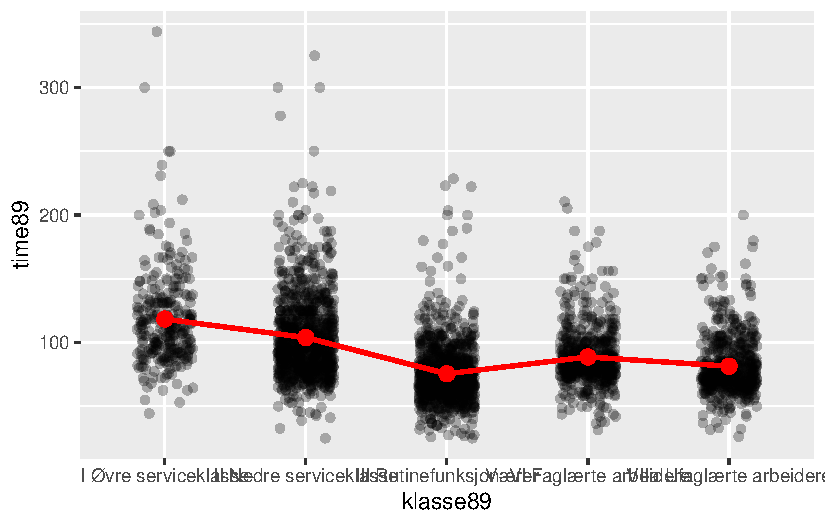
\includegraphics{./linearRegresjon_files/figure-pdf/unnamed-chunk-14-1.pdf}

}

\end{figure}

Den generelle regresjonsligningen skrives som \(y=a+bx\), der \(x\) er
forklaringsvariabelen. Regresjonskoeffisienten, \(b\), tolkes som hvor
forskjellen i gjennomsnittet på utfallsvariabelen, \(y\), mellom de som
er en enhets forskjell på \(x\)-variabelen.

Så kan vi kjøre en regresjon og få ut regresjonskoeffisientene på samme
måte som før. Akkurat her er \texttt{coef} lagt inn i en parentes for
\texttt{data.frame}, men det er bare for at det skal bli en pen kolonne.
Vi kommer altså tilbake til teknikker for penere output nedenfor.

\begin{Shaded}
\begin{Highlighting}[]
\NormalTok{est2 }\OtherTok{\textless{}{-}} \FunctionTok{lm}\NormalTok{(time89 }\SpecialCharTok{\textasciitilde{}}\NormalTok{ klasse89, }\AttributeTok{data =}\NormalTok{ abu89)  }
\FunctionTok{data.frame}\NormalTok{(}\FunctionTok{coef}\NormalTok{(est2)) }
\end{Highlighting}
\end{Shaded}

\begin{verbatim}
                                 coef.est2.
(Intercept)                       118.39851
klasse89II Nedre serviceklasse    -14.49078
klasse89III Rutinefunksjonærer    -42.89842
klasse89V-VI Faglærte arbeidere   -29.68788
klasse89VIIa Ufaglærte arbeidere  -36.95234
\end{verbatim}

Hvert estimat for kategori for klasse sammenlignes med \emph{den første
kategorien} (altså den som mangler): klasse I. Det betyr at klasse VII
(ufaglærte arbeidere) har en timelønn på -37 kroner mindre enn klasse I
(øvre serviceklasse). Mens klasse II (nedre serviceklasse) tjener -14.5
kroner mindre enn klasse I.

Forskjellen mellom andre grupper er således differansen mellom disse
estimatene. Altså: klasse VII tjener mindre enn klasse V-VI:
\(36.9 - 29.7 = 7.2\) kroner. Se på plottet over, så ser du at disse
tallene ser riktige ut.

\hypertarget{flere-variable}{%
\section{Flere variable}\label{flere-variable}}

Det er ikke så ofte vi bruker regresjon med bare en forklaringsvariabel,
såklat ``enkel lineær regresjon''.\footnote{Det er selvsagt ingenting
  \emph{enkelt} med slike modeller utover at det finnes mer kompliserte
  varianter.} Langt mer vanlig er å bruke flere variable samtidig i det
vi kaller ``multippel regresjon''.\footnote{Noen kaller dette også for
  \emph{multivariat} regresjon, men det er tvetydig da det også kan bety
  modeller med flere utfallsvariable, som er noe ganske annet.} I
multippel regresjon kan man altså beskrive mer kompliserte mønstre i
dataene.

Vi fortsetter med eksempelet om lønn og alder, men utvider med en
dimensjon til, nemlig kjønn. La oss først se på kjønnsforskjellene i
gjennomsnittlig timelønn.

\begin{Shaded}
\begin{Highlighting}[]
\NormalTok{abu89 }\OtherTok{\textless{}{-}}\NormalTok{ abu89 }\SpecialCharTok{\%\textgreater{}\%}
  \FunctionTok{mutate}\NormalTok{(}\AttributeTok{sex =} \FunctionTok{factor}\NormalTok{(}\FunctionTok{ifelse}\NormalTok{(female }\SpecialCharTok{==} \DecValTok{1}\NormalTok{, }\StringTok{"Female"}\NormalTok{, }\StringTok{"Male"}\NormalTok{), }\AttributeTok{levels =} \FunctionTok{c}\NormalTok{(}\StringTok{"Male"}\NormalTok{, }\StringTok{"Female"}\NormalTok{))) }\SpecialCharTok{\%\textgreater{}\%} 
  \FunctionTok{filter}\NormalTok{(}\SpecialCharTok{!}\FunctionTok{is.na}\NormalTok{(time89))}

\NormalTok{abu89 }\SpecialCharTok{\%\textgreater{}\%} 
  \FunctionTok{select}\NormalTok{(sex, time89) }\SpecialCharTok{\%\textgreater{}\%} 
  \FunctionTok{tbl\_summary}\NormalTok{(}\AttributeTok{by =}\NormalTok{ sex) }
\end{Highlighting}
\end{Shaded}

\begin{verbatim}
Table printed with `knitr::kable()`, not {gt}. Learn why at
https://www.danieldsjoberg.com/gtsummary/articles/rmarkdown.html
To suppress this message, include `message = FALSE` in code chunk header.
\end{verbatim}

\begin{longtable}[]{@{}
  >{\raggedright\arraybackslash}p{(\columnwidth - 4\tabcolsep) * \real{0.4054}}
  >{\centering\arraybackslash}p{(\columnwidth - 4\tabcolsep) * \real{0.2838}}
  >{\centering\arraybackslash}p{(\columnwidth - 4\tabcolsep) * \real{0.3108}}@{}}
\toprule()
\begin{minipage}[b]{\linewidth}\raggedright
\textbf{Characteristic}
\end{minipage} & \begin{minipage}[b]{\linewidth}\centering
\textbf{Male}, N = 2,003
\end{minipage} & \begin{minipage}[b]{\linewidth}\centering
\textbf{Female}, N = 1,756
\end{minipage} \\
\midrule()
\endhead
Gjennomsnittlig timelønn 1989 & 100 (32) & 79 (24) \\
\bottomrule()
\end{longtable}

Vi ser altså at menn hadde i gjennomsnitt høyere timelønn enn kvinner,
nærmere bestemt 21 kroner mer. Dette kan vi også undersøke med lineær
regresjon som følger:

\begin{Shaded}
\begin{Highlighting}[]
\NormalTok{lm\_est2 }\OtherTok{\textless{}{-}} \FunctionTok{lm}\NormalTok{(time89 }\SpecialCharTok{\textasciitilde{}}\NormalTok{ sex , }\AttributeTok{data =}\NormalTok{ abu89)}

\FunctionTok{coef}\NormalTok{(lm\_est2)}
\end{Highlighting}
\end{Shaded}

\begin{verbatim}
(Intercept)   sexFemale 
   99.84382   -20.75229 
\end{verbatim}

Det er altså slik at koeffisienten, \(\beta\), gir den samme differansen
som en enkel sammenligning av to gjennomsnitt.

Vi har allerede sett på alder og lønn, så vi kan utvide dette til å
inkludere kjønn samtidig i et scatterplot.

Grafisk er det da greit å bruke farger og slik vise for menn og kvinner
for seg. I \texttt{ggplot} spesifiseres da \texttt{group\ =\ sex} og at
fargene skal settes etter sammen grupperingen \texttt{col\ =\ sex} slik:

\begin{Shaded}
\begin{Highlighting}[]
\FunctionTok{ggplot}\NormalTok{(abu89, }\FunctionTok{aes}\NormalTok{(}\AttributeTok{x =}\NormalTok{ age, }\AttributeTok{y =}\NormalTok{ time89, }\AttributeTok{group =}\NormalTok{ sex, }\AttributeTok{col =}\NormalTok{ sex)) }\SpecialCharTok{+}
  \FunctionTok{geom\_jitter}\NormalTok{(}\AttributeTok{alpha =}\NormalTok{ .}\DecValTok{4}\NormalTok{)}
\end{Highlighting}
\end{Shaded}

\begin{figure}[H]

{\centering 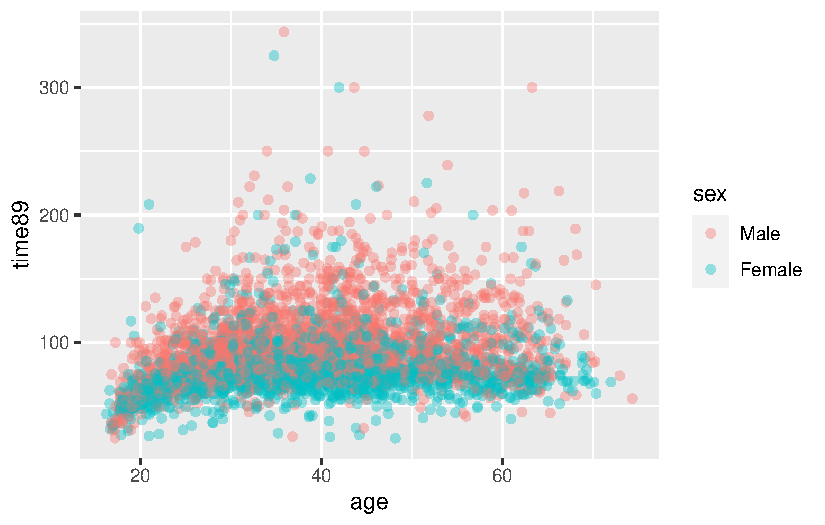
\includegraphics{./linearRegresjon_files/figure-pdf/unnamed-chunk-18-1.pdf}

}

\end{figure}

\begin{Shaded}
\begin{Highlighting}[]
\NormalTok{lm\_est3 }\OtherTok{\textless{}{-}} \FunctionTok{lm}\NormalTok{(time89 }\SpecialCharTok{\textasciitilde{}}\NormalTok{ sex }\SpecialCharTok{+}\NormalTok{ age, }\AttributeTok{data =}\NormalTok{ abu89)}

\FunctionTok{summary}\NormalTok{(lm\_est3)}
\end{Highlighting}
\end{Shaded}

\begin{verbatim}

Call:
lm(formula = time89 ~ sex + age, data = abu89)

Residuals:
   Min     1Q Median     3Q    Max 
-72.37 -17.12  -4.90  10.99 247.94 

Coefficients:
             Estimate Std. Error t value Pr(>|t|)    
(Intercept)  81.10147    1.58497   51.17   <2e-16 ***
sexFemale   -20.62511    0.91186  -22.62   <2e-16 ***
age           0.47380    0.03684   12.86   <2e-16 ***
---
Signif. codes:  0 '***' 0.001 '**' 0.01 '*' 0.05 '.' 0.1 ' ' 1

Residual standard error: 27.89 on 3756 degrees of freedom
Multiple R-squared:  0.1539,    Adjusted R-squared:  0.1535 
F-statistic: 341.7 on 2 and 3756 DF,  p-value: < 2.2e-16
\end{verbatim}

\hypertarget{prediksjon}{%
\section{Prediksjon}\label{prediksjon}}

Lineær regresjon kan også brukes til \emph{prediksjon} selv om dette i
liten grad er hva samfunnsvitere bruker regresjonsmodeller til.
Vanligvis vil vi primært være interessert i å tolke
regresjonskoeffisientene som sammenligninger mellom grupper. Man kan si
at man da er opptatt av \emph{forklaringsvariablene}. Når man predikerer
er man derimot opptatt av \emph{utfallsvariabelen}. Hvis man skulle være
interessert i temaer som maskinlæring, vil dette være en god inngang til
det.\footnote{f.eks. Et introduksjonskurs i maskinlæring som
  \href{https://www.uio.no/studier/emner/sv/iss/SOS2901/index.html}{SOS2901}
  starter gjerne med nettopp prediksjon med lineær regresjon.}

\hypertarget{regne-ut-forventet-verdi}{%
\subsection{Regne ut forventet verdi}\label{regne-ut-forventet-verdi}}

Merk at konstantleddet er tolkbart som forventet verdi på
utfallsvariabelen når alle andre prediktorer er null. I eksempelet
ovenfor med timelønn og klassetilhøringhet, er det altså ikke noen
koeffisient for klasse I. Gjennomsnittlig timelønn i klasse I er når de
andre dummyene er 0, altså 118.4 kroner. Gjennomsnittlig timelønn for
klasse II er tilsvarende 118.4 + (-14.49) = 103.9.

Hvis du skulle gjette timelønna til en person uten å vite noe annet enn
klasseposisjon ville det være fornuftig å gjette på gjennomsnittet for
denne klassen. Så vi kan bruke regresjonsmodeller til å regne ut
gjennomsnittslønn for gitte verdier av forklaringsvariable. I dette
eksempelet er det kanskje litt i overkant komplisert da vi jo også bare
kunne regnet ut gjennomsnittet per gruppe i en enkel tabell. Det ville
faktisk gitt akkurat samme resultat. Det er mer nyttig med kontinuerlige
variable og mer kompliserte modeller.

La oss se på regresjonsmodellen for hvordan timelønn varierer med alder
i stedet. Alder er kontinuerlig, så det er få personer på hvert
alderstrinn.

\begin{Shaded}
\begin{Highlighting}[]
\FunctionTok{coef}\NormalTok{(lm\_est1)}
\end{Highlighting}
\end{Shaded}

\begin{verbatim}
(Intercept)         age 
 71.1101883   0.4828415 
\end{verbatim}

Gjennomsnittlig timelønn ved 30 år vil da være 71.1 + 30 \(\times\) 0.5
= 86.1 kroner. Ved 35 år blir det tilsvarende 71.1 + 35 \(\times\) 0.5 =
88.6 kroner.

Dette kan vi altså regne ut for hånd, men man kan også bruke en
r-funksjon, nemlig \texttt{predict}. Denne funksjonen tar som argument
et regresjonsobjekt og en data.frame (altså et datasett eller
tilsvarende struktur) med samme variabelnavn som ble brukt i opprinnelig
regresjonsmodell.\footnote{Hvis man ikke spesifiserer data.frame brukes
  opprinnelige data og predikerer for hver person. Det kan man også
  gjøre for å f.eks. regne ut residualer, men vi gjør ikke det her nå.}

\hypertarget{predikere-for-kontinuerlig-variabel}{%
\subsection{Predikere for kontinuerlig
variabel}\label{predikere-for-kontinuerlig-variabel}}

Koden nedenfor lager først et datasett med én variabel: alder med noen
verdier man er interessert i utregning for. Så bruker man
\texttt{mutate} til å lage en kolonne til med predikerte verdier.

\begin{Shaded}
\begin{Highlighting}[]
\NormalTok{nyedata }\OtherTok{\textless{}{-}} \FunctionTok{data.frame}\NormalTok{(}\AttributeTok{age =} \FunctionTok{c}\NormalTok{(}\DecValTok{17}\NormalTok{, }\DecValTok{20}\NormalTok{, }\DecValTok{30}\NormalTok{, }\DecValTok{40}\NormalTok{, }\DecValTok{50}\NormalTok{, }\DecValTok{60}\NormalTok{))}

\NormalTok{nyedata }\SpecialCharTok{\%\textgreater{}\%} 
  \FunctionTok{mutate}\NormalTok{(}\AttributeTok{pred =} \FunctionTok{predict}\NormalTok{(lm\_est1, }\AttributeTok{newdata =}\NormalTok{ nyedata))}
\end{Highlighting}
\end{Shaded}

\begin{verbatim}
  age      pred
1  17  79.31849
2  20  80.76702
3  30  85.59543
4  40  90.42385
5  50  95.25226
6  60 100.08068
\end{verbatim}

\hypertarget{predikere-kategorisk-variabel}{%
\subsection{Predikere kategorisk
variabel}\label{predikere-kategorisk-variabel}}

Tilsvarende kan vi predikere for kategoriske variable slik som ble
benyttet i regresjonsmodellen for klasse. I det nye datasettet
spesifiseres f.eks. alle nivåene av en factor-variabel med funksjonen
\texttt{levels} og predikerer for disse.

\begin{Shaded}
\begin{Highlighting}[]
\NormalTok{nyedata }\OtherTok{\textless{}{-}} \FunctionTok{data.frame}\NormalTok{(}\AttributeTok{klasse89 =} \FunctionTok{levels}\NormalTok{(abu89}\SpecialCharTok{$}\NormalTok{klasse89))}

\NormalTok{nyedata }\SpecialCharTok{\%\textgreater{}\%} 
  \FunctionTok{mutate}\NormalTok{(}\AttributeTok{pred =} \FunctionTok{predict}\NormalTok{(est2, }\AttributeTok{newdata =}\NormalTok{ nyedata))}
\end{Highlighting}
\end{Shaded}

\begin{verbatim}
                  klasse89      pred
1     I Øvre serviceklasse 118.39851
2   II Nedre serviceklasse 103.90773
3   III Rutinefunksjonærer  75.50009
4  V-VI Faglærte arbeidere  88.71063
5 VIIa Ufaglærte arbeidere  81.44618
\end{verbatim}

\hypertarget{predikere-for-multippel-regresjon}{%
\subsection{Predikere for multippel
regresjon}\label{predikere-for-multippel-regresjon}}

Nytten av predict-funksjonen kommer mer til sin rett ved mer kompliserte
modeller. Her er et eksempel med flere variable:

Så kan vi regne ut estimert gjennomsnittlig verdi for de ulike
kombinasjonene av utvalgte verdier som følger:

\begin{Shaded}
\begin{Highlighting}[]
\NormalTok{nyedata }\OtherTok{\textless{}{-}} \FunctionTok{expand.grid}\NormalTok{(}\AttributeTok{age =} \DecValTok{30}\SpecialCharTok{:}\DecValTok{35}\NormalTok{, }
                      \AttributeTok{sex =} \FunctionTok{c}\NormalTok{(}\StringTok{"Female"}\NormalTok{, }\StringTok{"Male"}\NormalTok{))}
\NormalTok{nyedata }\SpecialCharTok{\%\textgreater{}\%} 
  \FunctionTok{mutate}\NormalTok{(}\AttributeTok{pred =} \FunctionTok{predict}\NormalTok{(lm\_est3, }\AttributeTok{newdata =}\NormalTok{ nyedata))}
\end{Highlighting}
\end{Shaded}

\begin{verbatim}
   age    sex     pred
1   30 Female 74.69049
2   31 Female 75.16429
3   32 Female 75.63810
4   33 Female 76.11190
5   34 Female 76.58571
6   35 Female 77.05951
7   30   Male 95.31560
8   31   Male 95.78940
9   32   Male 96.26320
10  33   Male 96.73701
11  34   Male 97.21081
12  35   Male 97.68462
\end{verbatim}

Funksjonen \texttt{predict} fungerer på tilsvarende måte uansett hvor
komplisert modellen måtte være. Men det kreves at det nye datasettet har
samme variabelnavn og variabeltype som i opprinnelige data.

\hypertarget{pene-tabeller-og-eksport-til-fil}{%
\section{Pene tabeller og eksport til
fil}\label{pene-tabeller-og-eksport-til-fil}}

Slik resultatene ser ut med bruk av \texttt{summary} er forsåvidt fint,
og du får den informasjonen du trenger. Men det er ikke særlig
presentabelt som ferdig produkt i en analyse. Du trenger typisk to ting:
1) Samle flere regresjonsmodeller i samme tabell, og 2) gjøre tabellene
penere og lettere å lese, og 3) eksportere til det
tekstbehandlingsprogrammet du bruker, typisk Microsoft Word.

R har en hel rekke funksjoner for dette. Det spiller egentlig ingen
rolle hvilke funksjoner du bruker da det er noe smak og behag her, så
det viktigste er at det fungerer rimelig greit for deg. Nedenfor
presenteres tre pakker for dette formålet. Velg én av dem. Hvis du ikke
har egne preferanser, så velg det første alternativet: \{modelsummary\}.
Alle disse funksjonene håndterer svært mange typer modeller, gir gode
muligheter for å ferdigstille tabellene fullstendig før eksport, og
eksporterer til de formatene som er mest aktuelle. De har også mer
avansert funksjonalitet som f.eks. å rapportere robuste standardfeil (av
forskjellig type) i stedet for vanlige standardfeil (dette er pensum på
SOS4020).

Vi vil som regel ha behov for å flytte resultatene over til et
tekstbehandlingsprogram. En strategi som går ut på ``klipp og lim''
eller skjermbilde etc er uaktuelt og må unngås for nærmest enhver
pris.\footnote{Hvis du blir tatt i å gjøre slikt vil faglærer sette fyr
  på datamaskinen din som straff.} Resultatene skal skrives til en fil
på en effektiv måte. Det er en fordel om tabellene da ser ganske ok ut i
utgangspunktet og du kan bruke samme prosedyre for å eksportere til
flere typer format hvis behovet skulle melde seg. Det er jo MS Word som
er viktigst for de fleste, mens de øvrige formatene nedenfor er for
spesielt interessert - men noen av dere vil kanskje bli det på et senere
tidspunkt. De viktigste formatene som er:

\begin{itemize}
\tightlist
\item
  MS Word - det vanligste tekstbehandlingsprogrammet som de aller fleste
  av dere bruker.
\item
  rtf - rikt tekstformat. Er et enklere format som fungerer på tvers av
  de fleste programmer. Kan brukes i Word også.
\item
  html - for websider
\item
  latex - for mer tekniske dokumenter, særlig hvis du har mye formler og
  stæsj
\item
  Markdown/Quarto - for dynamiske dokumenter med integrert R-kode og
  tekst, og kan eksportere ferdig dokument til alle ovennevnte
  formater\footnote{F.eks. dette dokumentet er skrevet i Quarto} Det som
  fungerer med Markdown fungerer også med Quarto for samme formål.
\end{itemize}

\hypertarget{alt-1-bruke-modelsummary}{%
\subsection{\texorpdfstring{Alt 1: Bruke
\texttt{modelsummary()}}{Alt 1: Bruke modelsummary()}}\label{alt-1-bruke-modelsummary}}

Eksporterer til bl.a. følgende formater: Word, rtf, html, latex,
markdown

Fordel: Gir pene og oversiktlige tabeller med enkel kode, og relativt
enkelt å modifisere videre. Eksporterer direkte til alle viktigste
formater. Kan også lett integreres med andre eksterne verktøy, først og
fremst ``grammar of tables'' i pakket \{gt\} Ulempe:

Her er kode for en enkel tabell med to regresjonsmodeller som vist
ovenfor. Merk at objektene med regresjonsresultatene må legges inni
funksjonen \texttt{list()}.

\begin{Shaded}
\begin{Highlighting}[]
\FunctionTok{library}\NormalTok{(modelsummary)}
\FunctionTok{modelsummary}\NormalTok{(}\FunctionTok{list}\NormalTok{(lm\_est2, lm\_est3))}
\end{Highlighting}
\end{Shaded}

\begin{table}
\centering
\begin{tabular}[t]{lcc}
\toprule
  & (1) & (2)\\
\midrule
(Intercept) & \num{99.844} & \num{81.101}\\
 & (\num{0.637}) & (\num{1.585})\\
sexFemale & \num{-20.752} & \num{-20.625}\\
 & (\num{0.932}) & (\num{0.912})\\
age &  & \num{0.474}\\
 &  & (\num{0.037})\\
\midrule
Num.Obs. & \num{3759} & \num{3759}\\
R2 & \num{0.117} & \num{0.154}\\
R2 Adj. & \num{0.116} & \num{0.153}\\
AIC & \num{35854.9} & \num{35694.9}\\
BIC & \num{35873.6} & \num{35719.8}\\
Log.Lik. & \num{-17924.434} & \num{-17843.437}\\
F & \num{496.278} & \num{341.699}\\
RMSE & \num{28.49} & \num{27.88}\\
\bottomrule
\end{tabular}
\end{table}

Denne tabellen inneholder mer enn du er interessert i. Nedre del av
tabellen inneholder ``goodness of fit'' statistikker, altså mål på
hvordan modellen passer til dataene. Det finnes mange slike, men ingen
grunn til å gå seg vill i disse her. De kan fjernes med argumentet
\texttt{gof\_omit\ =} og så angis statistikkene med de navnene du ser i
tabellen. Det skrives på en spesiell måte: som en tekststreng angitt med
anførselstegn rundt, og \texttt{\textbar{}} mellom hver. I koden
nedenfor beholdes kun antall observasjoner, \(r^2\) og \(F\).\footnote{Øvrige
  statistikker har selvsagt sitt bruksområde. De nevnte holder for de
  fleste formål.}

Vi gjør et par andre justeringer samtidig for å demonstrere noe
funksjonalitet. I stedet for å oppgi estimatet og standardfeil på
forskjellig linje kan vi spesifisere å ha det på samme linje med
argumentet \texttt{estimate\ =}. Merk at den statistikken du vil
rapportere settes i parentes \{\ldots\} og mellomrom og parentes er
ellers som det står. Man har også andre valg, derav det vanligste i bruk
er å angi \emph{p}-verdier eller \emph{stjerner} for å vise disse på en
forenklet måte. Det angis ved \texttt{\{p.value\}} eller
\texttt{\{stars\}} på tilsvarende måte.

I stedet for standardfeil på egen linje er det her angitt
konfidensintervall på neste linje. For konfidensintervall vil det som
forvalg være 95\%, men vi kan angi f.eks. 99\% konfidensintervall i
stedet ved \texttt{conf\_level\ =}. Hvis man ikke vil ha noe på neste
linje kan man angi \texttt{statistic\ =\ NULL} i stedet. Man kan også
velge å sette inn \texttt{p.value} eller \texttt{stars} på denne linjen.

Merk at utfallsvariabelen i modellene er timelønn i kroner. I forrige
tabell ble estimatene gitt med tre desimaler. Det er i overkant mange
desimaler. En desimal er mer passende og nedenfor endres dette med
\texttt{fmt\ =}.

\begin{Shaded}
\begin{Highlighting}[]
\FunctionTok{modelsummary}\NormalTok{(}\FunctionTok{list}\NormalTok{(lm\_est2, lm\_est3), }
             \AttributeTok{fmt =} \DecValTok{1}\NormalTok{,}
             \AttributeTok{estimate =} \StringTok{"\{estimate\} (\{std.error\})"}\NormalTok{,}
             \AttributeTok{statistic =} \StringTok{\textquotesingle{}conf.int\textquotesingle{}}\NormalTok{, }
             \AttributeTok{conf\_level =}\NormalTok{ .}\DecValTok{99}\NormalTok{, }
             \AttributeTok{gof\_omit =} \StringTok{\textquotesingle{}DF|Deviance|R2 Adj.|AIC|BIC|Log.Lik.|RMSE\textquotesingle{}}\NormalTok{)}
\end{Highlighting}
\end{Shaded}

\begin{table}
\centering
\begin{tabular}[t]{lcc}
\toprule
  & (1) & (2)\\
\midrule
(Intercept) & \num{99.8} (\num{0.6}) & \num{81.1} (\num{1.6})\\
 & {}[\num{98.2}, \num{101.5}] & {}[\num{77.0}, \num{85.2}]\\
sexFemale & \num{-20.8} (\num{0.9}) & \num{-20.6} (\num{0.9})\\
 & {}[\num{-23.2}, \num{-18.4}] & {}[\num{-23.0}, \num{-18.3}]\\
age &  & \num{0.5} (\num{0.0})\\
 &  & {}[\num{0.4}, \num{0.6}]\\
\midrule
Num.Obs. & \num{3759} & \num{3759}\\
R2 & \num{0.117} & \num{0.154}\\
F & \num{496.278} & \num{341.699}\\
\bottomrule
\end{tabular}
\end{table}

To siste ting å ta med her er å endre navn på variablene til noe mer
presentabelt og eksportere til Word. Med argumentet
\texttt{coef\_rename\ =} angis variabelen slik den ser ut i output og
spesifiserer hva du vil skal stå. Koden nedenfor viser eksempel.

For å eksportere til Word settes \texttt{output\ =} med filbane og
filnavn, og der filhalen \emph{.docx} angir Word format. Du kan
eksportere til annet format ved å angi annen filhale f.eks. .rtf eller
.html.

\begin{table}
\centering
\begin{tabular}[t]{lcc}
\toprule
  & (1) & (2)\\
\midrule
Konstant & \num{99.8} (\num{0.6}) & \num{81.1} (\num{1.6})\\
 & {}[\num{98.2}, \num{101.5}] & {}[\num{77.0}, \num{85.2}]\\
Kvinne & \num{-20.8} (\num{0.9}) & \num{-20.6} (\num{0.9})\\
 & {}[\num{-23.2}, \num{-18.4}] & {}[\num{-23.0}, \num{-18.3}]\\
Alder &  & \num{0.5} (\num{0.0})\\
 &  & {}[\num{0.4}, \num{0.6}]\\
\midrule
Num.Obs. & \num{3759} & \num{3759}\\
R2 & \num{0.117} & \num{0.154}\\
F & \num{496.278} & \num{341.699}\\
\bottomrule
\end{tabular}
\end{table}

\begin{Shaded}
\begin{Highlighting}[]
\FunctionTok{modelsummary}\NormalTok{(}\FunctionTok{list}\NormalTok{(lm\_est2, lm\_est3), }
             \AttributeTok{fmt =} \DecValTok{1}\NormalTok{,}
             \AttributeTok{estimate =} \StringTok{"\{estimate\} (\{std.error\})"}\NormalTok{,}
             \AttributeTok{statistic =} \StringTok{\textquotesingle{}conf.int\textquotesingle{}}\NormalTok{, }
             \AttributeTok{conf\_level =}\NormalTok{ .}\DecValTok{99}\NormalTok{, }
             \AttributeTok{gof\_omit =} \StringTok{\textquotesingle{}DF|Deviance|R2 Adj.|AIC|BIC|Log.Lik.|RMSE\textquotesingle{}}\NormalTok{, }
             \AttributeTok{coef\_rename =} \FunctionTok{c}\NormalTok{(}\StringTok{"sexFemale"} \OtherTok{=} \StringTok{"Kvinne"}\NormalTok{, }
                                   \StringTok{"age"} \OtherTok{=} \StringTok{"Alder"}\NormalTok{, }
                                  \StringTok{"(Intercept)"} \OtherTok{=} \StringTok{"Konstant"}\NormalTok{), }
             \AttributeTok{output =} \StringTok{"output/reg\_table.docx"}\NormalTok{)}
\end{Highlighting}
\end{Shaded}

Merk at Word vil vise tabellen med de fonter etc som er forvalgt for
Word. Dette kan du endre i Word etterpå. Det er en rekke funksjoner i
Word for å formattere tabeller som du kan bruke.

Pakken \{modelsummary\} har også en rekke andre funksjoner for å
redigere tabeller som du kan utforske ved behov. For avanserte brukere
kan man også gjøre om tabellen til et gt-objekt og redigere videre med
pakken \{gt\} eller tilsvarende med pakken \{flextable\}. Det er altså
tilnærmet uendelige muligheter for avanserte tabeller. Dette går
imidlertid langt utenfor hva de fleste av dere vil trenge.
\{modelsummary\} har
\href{https://vincentarelbundock.github.io/modelsummary/index.html}{egen
hjemmeside} med mer detaljer og instruksjoner.

\hypertarget{alt-2-bruke-stargazer}{%
\subsection{Alt 2: Bruke \{stargazer\}}\label{alt-2-bruke-stargazer}}

Mange R-brukere foretrekker pakken \{stargazer\}. Dette er en noe eldre
funksjon og er derfor godt etablert.

Eksporterer til bl.a. følgende formater: rtf, html, latex, markdown

Fordel: Er en stand-alone pakke men gir enkelt veldig fine tabeller som
antakeligvis er det du trenger Ulempe: Eksport til Word er ikke den
beste, men god nok.

Stargazer lager tabeller i kun tre formater: latex, html, og ren tekst.
Vi velger derfor \texttt{type\ =\ "text"} for at det skal se ok ut her.

\begin{Shaded}
\begin{Highlighting}[]
\FunctionTok{library}\NormalTok{(stargazer)}
\FunctionTok{stargazer}\NormalTok{(lm\_est2, lm\_est3, }\AttributeTok{type =} \StringTok{"text"}\NormalTok{)}
\end{Highlighting}
\end{Shaded}

\begin{verbatim}

=======================================================================
                                    Dependent variable:                
                    ---------------------------------------------------
                                          time89                       
                               (1)                       (2)           
-----------------------------------------------------------------------
sexFemale                  -20.752***                -20.625***        
                             (0.932)                   (0.912)         
                                                                       
age                                                   0.474***         
                                                       (0.037)         
                                                                       
Constant                    99.844***                 81.101***        
                             (0.637)                   (1.585)         
                                                                       
-----------------------------------------------------------------------
Observations                  3,759                     3,759          
R2                            0.117                     0.154          
Adjusted R2                   0.116                     0.153          
Residual Std. Error    28.495 (df = 3757)        27.891 (df = 3756)    
F Statistic         496.278*** (df = 1; 3757) 341.699*** (df = 2; 3756)
=======================================================================
Note:                                       *p<0.1; **p<0.05; ***p<0.01
\end{verbatim}

Vi kan modifisere tabellen tilsvarende som vi gjorde med
\{modelsummary\}. Forklaringer av de enkelte argumenter finnes i
\href{https://cran.r-project.org/web/packages/stargazer/stargazer.pdf}{manualen
for stargazer}.

\texttt{covariate.labels\ =} Angir teksten for variabelnavn. Merk at det
oppgis i den \emph{rekkefølgen} det skal stå, så være veldig nøye hvis
du har mange variable! \texttt{report\ =} angir hva som skal inngå i
tabellen, der hver bokstav viser til spesifikke deler: v = variabelnavn,
c = koeffisient/estimat, s = standardfeil. \texttt{single.row\ =} setter
statistikkene på samme linje fremfor under hverandre.
\texttt{keep.stat\ =} angir hvilke ``model fit statistics'' som skal
rapporteres. Hvis du skriver ``all'' her får du en lang remse
tilsvarende vi fikk med \{modelsummary\}. \texttt{digits\ =} angir
antall desimaler

\begin{Shaded}
\begin{Highlighting}[]
\FunctionTok{stargazer}\NormalTok{(lm\_est2, lm\_est3, }
          \AttributeTok{type =} \StringTok{"text"}\NormalTok{, }
          \AttributeTok{covariate.labels =} \FunctionTok{c}\NormalTok{(}\StringTok{"Kvinne"}\NormalTok{, }\StringTok{"Alder"}\NormalTok{, }\StringTok{"Konstant"}\NormalTok{),}
          \AttributeTok{report =} \StringTok{"vcs"}\NormalTok{,}
          \AttributeTok{single.row =} \ConstantTok{TRUE}\NormalTok{, }
          \AttributeTok{keep.stat =} \FunctionTok{c}\NormalTok{(}\StringTok{"n"}\NormalTok{,}\StringTok{"rsq"}\NormalTok{, }\StringTok{"ser"}\NormalTok{),}
          \AttributeTok{digits =} \DecValTok{1}\NormalTok{)}
\end{Highlighting}
\end{Shaded}

\begin{verbatim}

=====================================================
                           Dependent variable:       
                    ---------------------------------
                                 time89              
                          (1)              (2)       
-----------------------------------------------------
Kvinne                -20.8 (0.9)      -20.6 (0.9)   
Alder                                   0.5 (0.04)   
Konstant               99.8 (0.6)       81.1 (1.6)   
-----------------------------------------------------
Observations             3,759            3,759      
R2                        0.1              0.2       
Residual Std. Error 28.5 (df = 3757) 27.9 (df = 3756)
=====================================================
Note:                     *p<0.1; **p<0.05; ***p<0.01
\end{verbatim}

For å eksportere til Word kan man bruke rikt tekstformat (.rtf) eller
html. rtf-formatet er som navnet tilsier ren tekst og selv om det ser
greit ut, så er videre redigering i et tekstbehandlingsprogram krøkete.
(Prøv og se selv). Bruk heller html fordi da beholdes tabell-strukturen.
Du kan åpne html-tabeller fra Word og redigere videre der ved behov.

\begin{Shaded}
\begin{Highlighting}[]
\FunctionTok{stargazer}\NormalTok{(lm\_est2, lm\_est3, }
          \AttributeTok{type =} \StringTok{"text"}\NormalTok{,}
          \AttributeTok{covariate.labels =} \FunctionTok{c}\NormalTok{(}\StringTok{"Kvinne"}\NormalTok{, }\StringTok{"Alder"}\NormalTok{, }\StringTok{"Konstant"}\NormalTok{),}
          \AttributeTok{report =} \StringTok{"vcs"}\NormalTok{,}
          \AttributeTok{single.row =} \ConstantTok{TRUE}\NormalTok{, }
          \AttributeTok{keep.stat =} \FunctionTok{c}\NormalTok{(}\StringTok{"n"}\NormalTok{,}\StringTok{"rsq"}\NormalTok{, }\StringTok{"ser"}\NormalTok{),}
          \AttributeTok{digits =} \DecValTok{1}\NormalTok{, }
          \AttributeTok{out =} \StringTok{"output/reg\_starg.html"}\NormalTok{)}
\end{Highlighting}
\end{Shaded}

Mer detaljer finner du i
\href{https://cran.r-project.org/web/packages/stargazer/vignettes/stargazer.pdf}{\{stargazer\}
sin vignette}.

\hypertarget{alt-3-bruke-gtsummary}{%
\subsection{Alt 3: Bruke \{gtsummary\}}\label{alt-3-bruke-gtsummary}}

Vi har tidligere brukt \{gtsummary\} for å lage deskriptive tabeller,
som er det pakken er best til. Men den kan også lage gode
regresjonstabeller. Det er imidlertid en stor ulempe for nybegynnere i
R: det er ganske krøkete å sette sammen flere regresjonsmodeller i en
samlet tabell. Derfor er rådet å \emph{ikke bruke} denne pakken med
mindre du har veldig lyst til å prøve.

Fordel med å bruke denne pakken er at man slipper å lære enda en ny
pakke og slik sett ha ett sett med konsistent syntaks. En mulighet er
selvsagt å ikke lage tabellene så ferdig i R, men eksportere til Word og
redigere ferdig der mer manuelt.

\{gtsummary\} kan eksportere til følgende formater: Word, rtf, html,
latex og markdown. Resultatene kan også lett integreres med andre
funksjoner, først og fremst ``grammar of tables'' i pakket \{gt\} og
\{flextable\} - altså for mer avanserte ting som vi ikke dekker her.

Prinsippet er å lage hver tabell for seg og så slå dem sammen med
\texttt{tbl\_merge} etterpå. Det innebærer en del mer kode, rett og
slett. I utgangspunktet virker det ganske greit, men det er alltid en
del småting som krever litt mer.

Følgende kode lager først en ryddig tabell for hver regresionsmodell og
så kobler sammen disse to tabellene.

\begin{Shaded}
\begin{Highlighting}[]
\NormalTok{lm\_tab1 }\OtherTok{\textless{}{-}} \FunctionTok{tbl\_regression}\NormalTok{(lm\_est2, }\AttributeTok{intercept =}\NormalTok{ T, }
                          \AttributeTok{estimate\_fun =} \ControlFlowTok{function}\NormalTok{(x) }\FunctionTok{style\_number}\NormalTok{(x, }\AttributeTok{digits =} \DecValTok{1}\NormalTok{),}
                          \AttributeTok{show\_single\_row =} \StringTok{"sex"}\NormalTok{,}
                          \AttributeTok{label =} \FunctionTok{list}\NormalTok{(sex }\SpecialCharTok{\textasciitilde{}} \StringTok{"Kvinne"}\NormalTok{)) }\SpecialCharTok{\%\textgreater{}\%} 
    \FunctionTok{add\_glance\_table}\NormalTok{(}\AttributeTok{include =} \FunctionTok{c}\NormalTok{(nobs, r.squared, sigma))}
                     
\NormalTok{lm\_tab2 }\OtherTok{\textless{}{-}} \FunctionTok{tbl\_regression}\NormalTok{(lm\_est3, }\AttributeTok{intercept =}\NormalTok{ T,}
                          \AttributeTok{estimate\_fun =} \ControlFlowTok{function}\NormalTok{(x) }\FunctionTok{style\_number}\NormalTok{(x, }\AttributeTok{digits =} \DecValTok{1}\NormalTok{), }
                          \AttributeTok{show\_single\_row =} \StringTok{"sex"}\NormalTok{,}
                          \AttributeTok{label =} \FunctionTok{list}\NormalTok{(age }\SpecialCharTok{\textasciitilde{}} \StringTok{"Alder"}\NormalTok{, sex }\SpecialCharTok{\textasciitilde{}} \StringTok{"Kvinne"}\NormalTok{)) }\SpecialCharTok{\%\textgreater{}\%} 
    \FunctionTok{add\_glance\_table}\NormalTok{(}\AttributeTok{include =} \FunctionTok{c}\NormalTok{(nobs, r.squared, sigma)}
\NormalTok{  )}


\FunctionTok{tbl\_merge}\NormalTok{(}\AttributeTok{tbls =} \FunctionTok{list}\NormalTok{(lm\_tab1, lm\_tab2)) }\SpecialCharTok{\%\textgreater{}\%} 
  \FunctionTok{modify\_table\_body}\NormalTok{(}
    \SpecialCharTok{\textasciitilde{}}\NormalTok{.x }\SpecialCharTok{\%\textgreater{}\%} 
\NormalTok{      dplyr}\SpecialCharTok{::}\FunctionTok{arrange}\NormalTok{(}
\NormalTok{        row\_type }\SpecialCharTok{==} \StringTok{"glance\_statistic"}\NormalTok{, }\CommentTok{\# sort glance table to bottom}
\NormalTok{        var\_label                       }\CommentTok{\# sort by the variable label (a hidden column) }
\NormalTok{      )}
\NormalTok{  )}
\end{Highlighting}
\end{Shaded}

\begin{verbatim}
Table printed with `knitr::kable()`, not {gt}. Learn why at
https://www.danieldsjoberg.com/gtsummary/articles/rmarkdown.html
To suppress this message, include `message = FALSE` in code chunk header.
\end{verbatim}

\begin{tabular}{l|c|c|c|c|c|c}
\hline
**Characteristic** & **Beta** & **95\% CI** & **p-value** & **Beta** & **95\% CI** & **p-value**\\
\hline
(Intercept) & 99.8 & 98.6, 101.1 & <0.001 & 81.1 & 78.0, 84.2 & <0.001\\
\hline
Alder &  &  &  & 0.5 & 0.4, 0.5 & <0.001\\
\hline
Kvinne & -20.8 & -22.6, -18.9 & <0.001 & -20.6 & -22.4, -18.8 & <0.001\\
\hline
No. Obs. & 3,759 &  &  & 3,759 &  & \\
\hline
R² & 0.117 &  &  & 0.154 &  & \\
\hline
Sigma & 28.5 &  &  & 27.9 &  & \\
\hline
\end{tabular}

\hypertarget{lineuxe6r-sannsynlighetsmodell}{%
\chapter{Lineær
sannsynlighetsmodell}\label{lineuxe6r-sannsynlighetsmodell}}

\begin{Shaded}
\begin{Highlighting}[]
\FunctionTok{library}\NormalTok{(tidyverse)}
\FunctionTok{library}\NormalTok{(gtsummary)}
\end{Highlighting}
\end{Shaded}

I samfunnsvitenskapen har vi ganske ofte kategoriske variable både som
forklaringsvariable og utfallsvariable, eller en kombinasjon. I en
regresjon vil vi behandle kategoriske variable dem som om de er tall på
kontinuerlig akse, men der det typisk bare finnes to verdier: 0 og 1.
Dette kalles en dummyvariabel eller en indikatorvariabel.

Når man bruker kategoriske variable i en lineær regresjon er det derfor
ikke egentlig noe nytt. Det som står i læreboken om kontinuerlige
variable gjelder også for kategoriske variable (i hvert fall for alle
praktiske formål som dekkes for dette kurset).

\hypertarget{dummy-som-utfallsvariabel}{%
\section{Dummy som utfallsvariabel}\label{dummy-som-utfallsvariabel}}

I samfunnsvitenskapen er utfallsvariabelen ganske ofte kategorisk. I en
regresjon vil vi behandle kategoriske variable dem som om de er tall på
kontinuerlig akse, også der det typisk bare finnes to verdier: 0 og 1.
Dette kalles en dummyvariabel eller en indikatorvariabel.

Når man bruker kategoriske variable i en lineær regresjon er det derfor
ikke egentlig noe nytt. Det som står i boken om kontinuerlige variable
gjelder også for kategoriske variable (i hvert fall for alle praktiske
formål som dekkes for dette kurset).

Husk at tolkningen av regresjonskoeffisienten, \(b\), tolkes på den
skalaen \(y\)-variabelen er på. Altså: hvis utfallsvariabelen er i
kroner, så er tolkningen av \(b\) i måleenheten kroner. Hvis
y-variabelen er i antall timer, så er tolkningen av \(b\) i antall
timer, osv. Husk også at vi estimerer endring i gjennomsnitt.

Når utfallsvariabelen er en dummy, så har den verdiene 0 eller 1. Da er
gjennomsnittet det samme som en andel. For eksempel: hvis utfallet er om
man er i jobb eller ikke, og koder å være i jobb som 1 og 0 ellers. Hvis
man har 5 personer, derav 3 er i jobb får man så:
\(\bar{y} = \frac{(0+0+1+1+1)} {5} = \frac{3}{5}=0.6\) som er det samme
som 60\%.

I regresjon med slike variable er dermed utfallet en andel og dette
kalles derfor ofte en «lineær sannsynlighetsmodell». Men det er egentlig
en helt vanlig regresjonsmodell. Vi tolker fremdeles på den skalaen
y-variabelen er på, som altså er en andel. (Vi skal forresten senere
omtale andeler som estimater på sannsynligheter). En økning i
\(x\)-variabelen tilsvarer altså en endring, b, i andelen med den
egenskapen som er kodet 1 på \(y\)-variabelen.

La oss si at vi er interessert i å beskrive kjønnsforskjell i hvorvidt
menn og kvinner jobber i privat vs offentlig sektor. Variabelen
``private'' er en factor-variabel der første kategori er ``public'', som
da blir referansekategorien. R regner da privat sektor som 1 mens
offentlig sektor er 0. Koeffisientene vil da uttrykke forskjell i
sannsynlighet for å være i privat sektor.

\begin{Shaded}
\begin{Highlighting}[]
\FunctionTok{lm}\NormalTok{(private }\SpecialCharTok{\textasciitilde{}}\NormalTok{ female }\SpecialCharTok{+}\NormalTok{ ed }\SpecialCharTok{+}\NormalTok{ age, }\AttributeTok{data =}\NormalTok{ abu89)}
\end{Highlighting}
\end{Shaded}

\begin{verbatim}

Call:
lm(formula = private ~ female + ed + age, data = abu89)

Coefficients:
(Intercept)       female           ed          age  
   2.167030    -0.287998    -0.049017    -0.007274  
\end{verbatim}

Vi ser her at sannsynligheten for at kvinner jobber i privat sektor er
0.28 lavere enn for menn, dvs. 28 prosentpoeng lavere. Dette er da
kontrollert for utdanning og alder, slik at vi kan se bort fra at
utdanningsnivå og forskjell i aldersfordeling i dataene kan være grunnen
til forskjellene.

\part{Del 4: statistisk tolkning}

\hypertarget{design-og-tolkning}{%
\chapter{Design og tolkning}\label{design-og-tolkning}}

\hypertarget{tre-nivuxe5er-av-regresjonanalyse}{%
\section{Tre nivåer av
regresjonanalyse}\label{tre-nivuxe5er-av-regresjonanalyse}}

Richard Berk beskriver i sin lærebok tre nivåer av regresjonsanalyse
basert på hvordan dataene ble til. Dette er et godt utgangspunkt som
burde klargjøre betydelig, i hvert fall som et først skritt.

\hypertarget{nivuxe5-i-ikke-tilfeldig-utvalg-fra-en-veldefinert-populasjon}{%
\subsection{Nivå I: Ikke tilfeldig utvalg fra en veldefinert
populasjon}\label{nivuxe5-i-ikke-tilfeldig-utvalg-fra-en-veldefinert-populasjon}}

Grunnlaget for statistisk tolkning (sannsynligheter, p-verdier og sånn)
er at dataene er en tilfeldig realisering av en underliggende sann
verdi. Typisk betyr dette bare at man har trukket et tilfeldig utvalg
fra en populasjon. Da vil man få et godt mål på f.eks.
gjennomsnittsverdi i populasjonen, men på grunn av tilfeldighet vil det
være en feilmargin på denne målingen.

Det avgjørende er altså at det finnes en veldefinert populasjon som det
kan generaliseres til. Grunnen til å bruke begrepet \emph{veldefinert}
er at det må være rimelig spesifisert.

Hvis dataene \emph{ikke} er fra en veldefinert populasjon kalles dette
noen ganger for \emph{convenience sample}. Altså, at man gjorde et
uttrekk av beleilighetsgrunner, men uten at det var en veldefinert
populasjon.

Et eksempel kan være en arbeidsmiljøundersøkelse i en bestemt bedrift.
Det skal litt til at disse resultatene skal gjelde utover denne
bedriften. Man kan selvsagt argumentere for at erfaringene gjelder med
generelt, men en slik slutning vil da hvile først og fremst på disse
argumentene - ikke på statistiske utregninger.

Det kan være veldig nyttig å analysere slike data, og det kan bringe
innsikt og kunnskaper. Men med slike data gir det ikke mye mening å
regne på statistisk usikkerhet. Hvis man ikke skal si noe utover de
dataene man har (ikke generalisere), så er det heller ikke denne typen
usikkerhet i målingene.

Slike ikke-tilfeldige utvalg kan betraktes nærmest som case-studier. En
dataanalyse vil gi oss kunnskaper om de erfaringene som gjøre akkurat
der. Størrelsen på datasettet kan gi oss mer pålitelig informasjon om
dette caset, men hjelper ikke for å generalisere utover caset.

\hypertarget{nivuxe5-ii-tilfeldig-utvalg-fra-en-veldefinert-populasjon}{%
\subsection{Nivå II: Tilfeldig utvalg fra en veldefinert
populasjon}\label{nivuxe5-ii-tilfeldig-utvalg-fra-en-veldefinert-populasjon}}

Tilfeldig utvalg er akkurat det det høres ut som, og er den foretrukne
metoden for alle surveyundersøkelser. Teorien bak er at utvalget vil
gjenspeile populasjonen, og avvik fra ``de sanne verdiene'' skyldes
tilfeldigheter. Disse tilfeldighetene er grunnlaget for statistisk
tolkning ved at vi kan si noe om \emph{samplingfordelingen} (se annet
kapittel) og dermed har grunnlag for å regne på standardfeil og
p-verdier osv. Med andre ord: generalisering til populasjonen.

Så er det viktig å påpeke at forutsetningen her er at det må være et
utvalg fra en \emph{veldefinert} populasjon. Hvis vi ikke vet hvem
resultatene generaliserer til, så blir det jo tullete, og vi er egentlig
på nivå 1.

\hypertarget{nivuxe5-iii-estimering-av-kausale-effekter}{%
\subsection{Nivå III: Estimering av kausale
effekter}\label{nivuxe5-iii-estimering-av-kausale-effekter}}

Fra et teknisk perspektiv er det ingenting som skiller studier av
eksperimenter fra observasjonsstudier. De samme regresjonsmodellene kan
estimeres og de samme utregningene av usikkerhet. Hva som bestemmer
tolknigen (og hvorvidt modellspesifikasjonen er rimelig etc) avhenger av
forskningsdesignet. Kort sagt kreves det et eksperiment. Hvis man har en
\emph{treatment}-gruppe og en kontrollgruppe, så vil \(\beta\) beskrive
forskjellen mellom disse gruppene som i andre typer data. Det som gir
\(\beta\) en \emph{kausal} tolkning er om dataene tilfredsstiller
kravene til et eksperiment.

Vi kan også regne inn kvasi-eksperimentelle studier eller naturlige
eksperimenter her. Enten er disse studiene gode nok til å kvalifisere
til å tolke som kausaleffekter - eller så er de det ikke, men da hører
de hjemme på nivå II.

\hypertarget{mot-et-nivuxe5-iv}{%
\subsection{Mot et nivå IV?}\label{mot-et-nivuxe5-iv}}

I Berk sin fremstilling av de tre nivåene får man en følelse av at den
vitenskapelige verdien øker ved hvert nivå. Mange vil da også mene
akkurat det. Men logisk sett er det litt mer tvetydig enn som så.

Vi har snakket om to dimensjoner: kausalitet (ja/nei) og generalisering
(ja/nei). Dette gir fire logisk mulige kombinasjoner.

\hypertarget{tbl-}{}
\begin{longtable}[]{@{}
  >{\raggedright\arraybackslash}p{(\columnwidth - 4\tabcolsep) * \real{0.2500}}
  >{\raggedright\arraybackslash}p{(\columnwidth - 4\tabcolsep) * \real{0.3889}}
  >{\raggedright\arraybackslash}p{(\columnwidth - 4\tabcolsep) * \real{0.3611}}@{}}
\caption{\label{tbl-}Nivåer av regresjonsanalyse og hvor vanlige de
er}\tabularnewline
\toprule()
\begin{minipage}[b]{\linewidth}\raggedright
\end{minipage} & \begin{minipage}[b]{\linewidth}\raggedright
Ikke tilfeldig utvalg fra veldefinert populasjon
\end{minipage} & \begin{minipage}[b]{\linewidth}\raggedright
Tilfeldig utvalg fra veldefinert populasjon
\end{minipage} \\
\midrule()
\endfirsthead
\toprule()
\begin{minipage}[b]{\linewidth}\raggedright
\end{minipage} & \begin{minipage}[b]{\linewidth}\raggedright
Ikke tilfeldig utvalg fra veldefinert populasjon
\end{minipage} & \begin{minipage}[b]{\linewidth}\raggedright
Tilfeldig utvalg fra veldefinert populasjon
\end{minipage} \\
\midrule()
\endhead
Deskriptiv & Overraskende mange & Det aller meste \\
Kausal & Mye, men burde nok vært mer & Ganske sjelden \\
\bottomrule()
\end{longtable}

Jeg har ingen empiri for å si hvor vanlig hver enkelt type analyse er.
Men jeg tror det nokså omtrentlige angivelsen i tabellen er ganske
riktig, basert på egen erfaring fra studier jeg har lest og
presentasjoner jeg har sett.

I Berk sin fremstilling er Nivå III hele nederste rad, men da er det
altså ikke gjort skille mellom om resultatene kan generaliseres videre
eller ikke. Et slik skille bør man nok gjøre.

Eksperimenter omtales noen ganger - og i noen fagmiljøer - som
\emph{gullstandarden}. Men altså: ethvert eksperiment kan ikke være en
gullstandard, ikke engang når formålet er å estimere kausaleffekter.
Nivå IV er i så fall det vi ser etter, da nivå III har begrenset
gyldighet. I tilsvarende ånd omtaler Berk eksperimenter som
\emph{bronsestandarden}, med den begrunnelse at det i praksis ikke er
noe på palleplassene sølv og gull.

\hypertarget{hva-er-poenget-her-egentlig}{%
\section{Hva er poenget her,
egentlig?}\label{hva-er-poenget-her-egentlig}}

Poenget er at tolkning av resultatene handler vel så mye om hvordan
dataene har \emph{blitt til} som hvordan de er \emph{analysert}. Hvis du
har data på nivå I, så finnes det ingen statistiske krumspring du kan
gjøre som løfter det til et annet nivå. Det samme gjelder nivå II og
nivå III. Du kan fremdeles gjøre svært så nyttige og informative
analyser på det nivået du har data på. De statistiske analyseteknikkene
er det ellers ikke så stor forskjell på.

\hypertarget{hva-med-sosiologisk-teori}{%
\section{Hva med sosiologisk teori?}\label{hva-med-sosiologisk-teori}}

Vi bruker kvantitative metoder til å beskrive statistiske sammenhenger.
Men vi er jo ikke interessert i \emph{variablene} som sådan. Poenget er
å beskrive sosiale fenomener. Å si hva det betyr krever imidlertid en
teoretisk tolkning. Å teste om et estimat er statistisk signifikant er
ikke det samme som å teste en teori, selv om begge deler kan omtales med
ordet ``test''.

\begin{itemize}
\tightlist
\item
  Gitt et fenomen (beskrevet med statistikk), hvordan kan vi forklare
  det?
\item
  Hva skjer med fenomenet vi er interessert i hvis vi gjør en
  intervensjon?
\item
  Gitt en teori, er observasjonsdata (dvs. statistikk) konsistent med
  teorien?
\item
  Gitt en teori, kan vi sjekke om observasjonsdata (dvs. statistikk)
  \emph{ikke} er konsistent med teorien?
\end{itemize}

Den første varianten handler om å først beskrive - gjerne eksplorerende
- og så bruke teori til å forklare hvorfor det er slik. Det følger
gjerne flere analyser som gjør beskrivelsen mer nyanserte og utforsker
ulike muligheter.

Den andre varianten handler om å måle effekter, gjerne et naturlig
eksperiment eller et felteksperiment. Hvis man ønsker å vite hva
\emph{effekten} av et tiltak er, så må man endre noe slik at man kan
observere resultatet. Randomisering handler om å håndtere seleksjon.

Den tredje varianten er en konfirmerende strategi: En teori bør jo være
konsistent med hvordan verden ser ut. Det er viktig å sjekke at dette er
tilfellet. Hvis det er konsistent vet man jo det, men det er ikke en
\emph{test} av noe som helst fordi det kan jo være alternative teorier
som forklarer minst like godt.

Den fjerde varianten krever at teorien gir en \emph{empirisk
forventning} - helst som er motstridende med en annen teori. Hvis det
kan vises empiriske mønster som er inkonsistente med teori, så må
teorien enten forkastes eller i det minste justeres. Hvor mye vil være
helt avhengig av den teoretiske påstanden.

\emph{Statistiske tester}, med p-verdier og konfidensintervaller, brukes
til å skille mellom tilfeldig variasjon og systematisk variasjon på en
tilsvarende måte for alle strategier.

\hypertarget{statistisk-tolkning}{%
\chapter{Statistisk tolkning}\label{statistisk-tolkning}}

Det vi omtaler som \emph{statistisk tolkning} eller \emph{statistisk
inferens} handler om å skille systematikk fra støy. Altså: håndtering av
usikkerhet ved estimeringen. Dette er relevant for analyser på nivå II
og III (se forrige kapittel). På nivå II handler det om å
\emph{generalisere} til en veldefinert populasjon, mens det på nivå III
handler om å si om en kausal effekten kan skilles fra tilfeldig støy. De
statistiske teknikken er imidlertid de samme. I praksis handler dette om
(på dette nivået) følgende:

\begin{enumerate}
\def\labelenumi{\arabic{enumi})}
\tightlist
\item
  standardfeil
\item
  konfidensintervall
\item
  p-verdi
\end{enumerate}

Disse tre henger nøye sammen og er forskjellige uttrykk for
\emph{feilmarginen} ved et estimat. Her skal vi ikke gjennomgå
begrunnelsene og det teoretiske grunnlaget for hvordan dette fungerer,
men hoppe rett til det praktiske. En skikkelig forklaring følger fra
\emph{sentralgrenseteoremet}\footnote{Hvis detter ukjent stoff for det
  kan du se en som er dekket i f.eks. Moore Notz og Fligner (2021)
  \emph{The basic practice of statistics}, kapittel 15, etterfulgt av
  forlengelsen til konfidensintervall og statistiske tester i kapittel
  16 og 17.}.

Litt enkelt kan vi si at det hvis man gjør en studie på en ordenlig
måte, så er ganske sannsynlig at man får en estimat som er lik den sanne
verdien. Men det er også ganske \emph{lite sannsynlig} at man får et
estimat som er \emph{nøyaktig} lik den sanne verdien. Vi må regne med at
estimatet avviker noe på grunn av \emph{tilfeldigheter}! Det er veldig
nyttig å vite noe om hvor mye feil man kan forvente å få av tilfeldige
grunner. Altså: hva er feilmarginen til den metoden vi bruker til å
estimere?

Denne feilmarginen avhenger først og fremst av hvordan undersøkelsen er
gjennomført. Utvalgsprosedyren er det viktigste: tilfeldig trukket
utvalg er det mest grunnleggende momentet. Hvis det er systematiske
skjevheter i dataene, så vil estimatet bli systematisk skjevt på måter
vi ikke så lett kan håndtere med statistiske teknikker.

Dernest avhenger feilmarginen av utvalgsstørrelsen. Det er rett og slett
slik at større data gir sikrere estimatet. Hvis utvalget består av 10
personer, så vil estimatet være langt mer usikkert enn hvis det hadde
bestått av 5000 personer. Selv om det finnes en statistisk forklaring på
dette, så er det relativt intuitivt å forstå. I utregninger vil
standardfeilen bli mindre hvis antall observasjoner er større.

Til sist avhenger feilmarginen av en grense vi selv setter, som gjerne
kalles \emph{konfidensgrad}. Denne setter vi selv, men det er vanlig å
sette denne til 95\%. Det gjør at man noen ganger sier ``95\% sikker'',
hvilket er en nokså sleivete måte å si det på, men ikke helt galt under
visse forutsetninger som vi kommer tilbake til.

\hypertarget{estimater-og-feilmarginer}{%
\section{Estimater og feilmarginer}\label{estimater-og-feilmarginer}}

\hypertarget{estimat}{%
\subsection{Estimat}\label{estimat}}

La oss si at du ønsker å si noe om gjennomsnittet i \emph{populasjonen},
men har bare data om et tilfeldig \emph{utvalg} fra denne populasjonen.
Når du da regner ut gjennomsnittet i utvalget er det din beste gjetning
på hva gjennomsnittet er i populasjonen. En slik gjetning kaller vi et
\emph{estimat}.

\hypertarget{standardfeil}{%
\subsection{Standardfeil}\label{standardfeil}}

Standardfeilen uttrykker usikkerheten ved \emph{estimatet}.
Standardfeilen til estimatet er et mål på usikkerheten ved målemetoden.
Usikker målemetode gjør at feilen kan være større.

Ordet standard\emph{feil} er lett å blande sammen med
standard\emph{avvik}, så la oss ta det med det samme. Standardavviket
beskriver variasjon i data, f.eks. hvis man vil beskrive hvordan
personers inntekt varierer rundt gjennomsnittet. Standardavviket
beskriver altå variasjon i \emph{data}.

Standard\emph{feilen} beskriver derimot ikke data, men
sannsynlighetsfordelingen for hvordan vi forventer at \textbf{estimatet}
vil kunne avvike fra den sanne verdien på grunn av tilfeldigheter.

Sentralgrenseteoremet sier at estimatet på et gjennomsnitt vil ha
tilfeldige feil som er \emph{normalfordelt}, og dermed kan vi bruke
normalfordelingen til å si noe om usikkerheten ved estimatet. Dette er
forsøkt illustrert nedenfor der x-aksen viser hvor mye estimatet kan
avvike fra den sanne verdien, mens kurven viser hvor
sannsynligsfordelingen til avviket. Den stiplede linjen viser den sanne
verdien. Når x-aksen er avvik fra sanne verdien, så vil altså \(x = 0\)
bety null avvik fra sanne verdien: helt riktig estimat.

Altså: det er aller mest sannsynlig å få et estimat som ligger nærme den
sanne verdien, men litt avvik (større eller lavere estimat) er nesten
like sannsynlig. Jo lengre til hver av sidene man går (større feil), jo
mindre sannsynlig er det å få et slikt estimat.

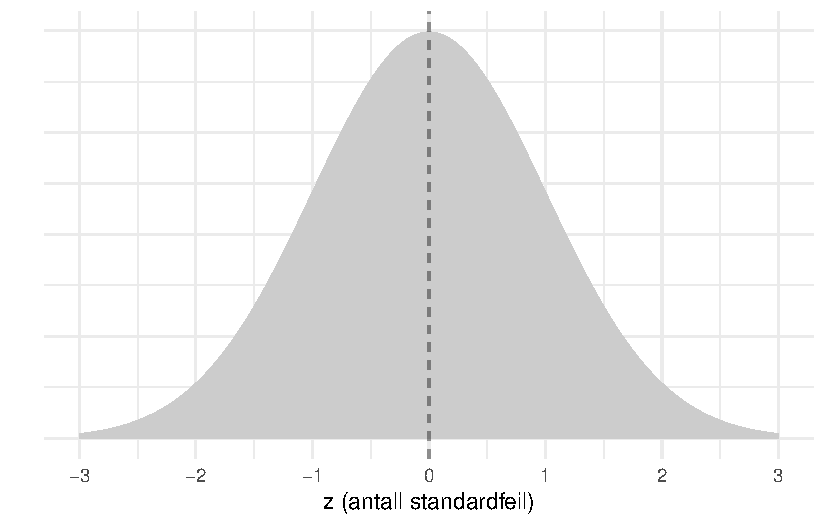
\includegraphics{./statistiskTolkning_files/figure-pdf/unnamed-chunk-1-1.pdf}

Skalaen på x-aksen er \(z\), som i denne sammenheng kan tolkes som
antall standardfeil. Den følger en standard normalfordeling som har
kjente og faste egenskaper. Vi vet f.eks. at andelen \emph{nedenfor}
-1.96 er 0.025, og det samme gjelder \emph{ovenfor} 1.96. Dette er
illustrert i figuren nedenfor. Det er altså 0.05 (dvs 5\%) sannsynlighet
for å få et estimat som ligger 1.96 standardfeil unna den sanne verdien.
Motsatt er sannsynligheten for å få et estimatet innenfor intervallet
mellom -1.96 og 1.96 tilsvarende 95\%. Dette er grunnlaget for det vi
kaller \emph{konfidensintervall}.

\includegraphics{./statistiskTolkning_files/figure-pdf/unnamed-chunk-2-1.pdf}

\hypertarget{konfidensintervall}{%
\subsection{Konfidensintervall}\label{konfidensintervall}}

Hvis man ønsker å være ``95\% sikker'', så bruker man altså et 95\%
konfidensintervall. Det er ikke noe magisk ved akkurat 95\% og er
primært blitt en norm. Grunnen er bare at det skal være en ganske lav
sannsynlighet for at estimatet skyldes tilfeldig variasjon.

Til ethvert estimat er knyttet en feilmargin som uttrykkes ved
\(z \times se\), der \(se\) er forkortelse for standardfeil (engelsk:
``standard error''). \(z\) er et tall som er knyttet til grad av
usikkerhet ved feilmarginen. En feilmargin basert på 95\% konfidensgrad
er dermed \(1.96 \times se\). Hvis man så tar denne feilmarginen til
hver side, så gir det samme som illustrert i figuren ovenfor.

Et konfidensintervall er altså bare å ta hensyn til feilmarginen til
hver side av estimatet. Når vi bruker dette i praksis baserer vi oss på
denne normalfordelingen og trenger bare å få regnet ut standardfeilen i
tillegg.

\begin{verbatim}
[1] 91.0712
\end{verbatim}

Hvis man f.eks. har estimert gjennomsnittlig timelønn til å være 90.2 og
standardfeilen er 0.5. Da blir 95\% konfidensintervallet som følger:

\[ 90.1 \pm 1.96 \times 0.47 = [89.2, 91.1]\] Dette betyr at vi har
brukt en målemetode som har en feilmargin som gjør at vi kan være 95\%
sikker på at den sanne verdien ligger innenfor dette intervallet.

\hypertarget{er-man-egentlig-95-sikker}{%
\subsubsection{Er man egentlig ``95\%
sikker''?}\label{er-man-egentlig-95-sikker}}

Det sies ofte at feilmarginen uttrykker hvor sikker man er. Det er jo
ikke helt riktig - eller det er riktig under noen spesielle
forutsetninger om hva man mener med ``sikker''. La oss derfor ta dette
med en gang.

Et 95\% konfidensintervall er vårt anslag på hvor god vår
\emph{målemetode} er. Vi har jo regnet ut f.eks. et gjennomsnitt og det
er jo greit nok. Usikkerheten kommer fra utvalgsprosedyren og
variasjonen i data.

Vi vet ikke hvorvidt vårt estimat ligger nærme eller langt unna den
sanne verdien. Det vi derimot vet noe om er påliteligheten i den metoden
vi har brukt. Det viktigste her er altså tilfeldig utvalg, og hvis
utvalget ikke er tilnærmet tilfeldig trukket, så bryter det hele sammen.

Når man sier at konfidensintervallet uttrykker at man er ``95\% sikker''
på at den sanne verdien ligger i det intervallet mener man da følgende:
Man har brukt en \emph{metode} (dvs utvalg og utregninger og det hele)
som har en \emph{feilmargin}. Denne feilmarginen er slik at hvis man
gjorde estimeringen (altså nytt utvalg hver gang) på samme måte svært
mange ganger (f.eks. uendelig mange ganger), så ville 95\% av
resultatene ligget innenfor et slikt intervall.

Man gjør selvsagt ikke samme undersøkelse tusenvis av ganger, så dette
er en hypotetisk tanke. Man man kan også tenke seg at mange ulike
forskere gjør en tilsvarende studie og får litt forskjellige resultat.
Disse resultatene vil (i teorien) fordele seg som en normalfordeling
rundt den sanne verdien. Noen ganske få vil ligge langt unna sannheten.

\hypertarget{t-testen}{%
\subsection{T-testen}\label{t-testen}}

Hvis man skal sammenligne to grupper, så vet vi i utgangspunktet at
dataene fra et utvalg antakeligvis vil vise at de ikke er helt like på
grunn av tilfeldig variasjon. Det kan altså være at gruppene er like i
virkeligheten, bare at dataene våre tilfeldigvis ble litt forskjellige.
Det må vi jo regne med, men det er begrenset hvor forskjellig vi kan
forvente at gruppene er på grunn av rene tilfeldigheter.

Se igjen på figuren over av normalfordelingen i omtalen av
konfidensintervall. Gitt at det ikke er noen sann forskjell mellom
gruppene, så vil vi forvente at estimatet ligger \emph{innenfor} en viss
feilmargin. Det betyr at en observert forskjell i dataene som ligger
\emph{innenfor} denne feilmarginen vil være konsistent med at
forskjellene bare skyldes tilfeldig variasjon. Motsatt: hvis estimatet
ligger \emph{utenfor} denne feilmarginen, ja da kan vi si at det ikke er
konsistent med dette utgangspunktet om at forskjellene bare skyldes
tilfeldig variasjon.

En av de meste brukte statistiske testene i praksis er ``t-testen''. Du
kan tenke på det som en \textbf{beslutningsregel}: hva skal til for at
du skal bestemme deg for å tro at forskjellen \emph{ikke skyldes
tilfeldigheter}? Standardfeil og feilmarginer er det samme som før, så
du må bare bestemme deg for hvor stor feilmargin du er villig til å
operere med. Hvis estimatet på en differanse er \emph{større} enn
feilmarginen, da forkastes hypotesen om at forskjeller skyles
tilfeldigher. Altså: forskjellene i data må da skyldes noe mer
systematisk.

Så i utgangspunktet så må du altså ta stilling til om du mener det er en
forskjell - eller ikke. Du kan ikke konkludere med at det ``kanskje er
en forskjell'', men må ta et valg. Derfor kaller vi gjerne dette for
hypotesetesting i en litt snever forstand. Det er bare to mulige
hypoteser:

\(H_0\): Det er egentlig ingen forskjell mellom gruppene, og forskjell i
\emph{dataene} skyldes bare tilfeldig variasjon. (Nullhypotesen).
\(H_A\): Det er faktisk en forskjell mellom gruppene, og forskjellen i
\emph{dataene} er for stor til av det er sannsynlig at det skyldes
tilfeldig variasjon. (Alternativ hypotese).

\hypertarget{formler-og-slikt}{%
\subsubsection{Formler og slikt}\label{formler-og-slikt}}

T-testen i prinsippet en sammenligning mellom estimatets størrelse og
standardfeilen til estimatet. Vi kan skrive det som følger:

\[
 \frac{\mu}{SE(\mu)} = t 
\]

Eller sagt på en annen måte: \[
 \frac{estimat}{standardfeil} = t 
\]

Det betyr at \(t\)-verdien egentlig bare er forholdstallet mellom
estimatet og standardfeilen. Intuitivt kan man vel forstå at hvis
usikkerheten bør være mindre enn estimatet. Altså: hvis du har estimert
en forskjell i timelønn mellom to grupper, og feilmarginen til dette
estimatet er større enn forskjellen, ja, da er det vanskelig å lære noe
særlig fra det estimatet.

Verdien \(t\) tilsvarer verdien \(z\) som vi nevnte i forbindelse med
konfidensintervall. Så hvis \(t\) er større enn \(z\), så ligger
estimatet \emph{utenfor} konfidensintervallet.

Tolkningen av \(t\)-verdien brukes gjerne som en en beslutningsregel:
Ja/Nei. Litt firkantet, med andre ord. Men \(t\)-verdien er også knyttet
til normalfordelingen på samme måte som nevnt ovenfor i forbindelse med
konfidensintervaller. Ethvert mulig resultat er knyttet til en viss
sannsynlighet for at det skal skje ved en tilfeldighet.

\hypertarget{p-verdi}{%
\subsubsection{P-verdi}\label{p-verdi}}

Tolkningen av p-verdien er i hvilken grad det er sannsynlig å få det
observerte resultatet \emph{ved en tilfeldighet} hvis NULL-hypotesen er
riktig. Dette høres ganske pussig ut. Tanken er at man nesten alltid vil
observere noe forskjell fra null, og det kan skje ved en tilfeldighet.
Hvis null-hypotesen er riktig er det mindre sannsynlig at vi observerer
en veldig stor forskjell. Men hvor stor forskjell er det, egentlig?
Løsningen er å se avstanden fra null i lys av standardfeilen. Hvis man
bruker en usikker målemetode, så er det mer sannsynlig å observere en
stor forskjell ved tilfeldigheter enn om man bruker en veldig nøyaktig
målemetode.

I praksis: Tenk at du observerer en stor forskjell mellom to grupper.
Med ``stor'' mener vi f.eks. at forskjellen er over dobbelt så stor som
standardfeilen. Da får vi en p-verdi som er \(p < 0.05\). Da kan vi si
at hvis nullhypotesen er sann, så er det lite sannsynlig at vi ville
fått et slikt resultat på grunn av tilfeldigheter.\^{}(Hvis vi ønsker
være pinlig korrekte kan vi også si noe slikt som at hvis man gjorde
målingen tusenvis av ganger, så ville 5\% av resultatene ligge så langt
unna null (eller lengre).)

Så er logikken videre at vi som hovedregel ikke tror på resultater som
er usannsynlige. Så i stedet for å holde fast på nullhypotesen velger vi
i stedet å tro på den alternative hypotesen.

\hypertarget{kan-man-velge-fritt-konfidensgrad}{%
\section{Kan man velge fritt
konfidensgrad?}\label{kan-man-velge-fritt-konfidensgrad}}

Det er ingenting magisk med tallet 1.96 eller \(p < 0.05\). Det er en
konvensjon. Konfidensgrad er nemlig noe \emph{du} velger. All tolkning
av ``statistisk signifikans'' er basert på en gitt konfidensgrad.

Problemet oppstår hvis du først ser på resultatene og så velger en
konfidensgrad som passer til det du har mest lyst til å konkludere med.
Det er rett og slett juks. For at du skal velge en annen konfidensgrad
må du si det høyt og tydelig \emph{før} du gjennomfører undersøkelsen -
og da må du faktisk etterleve det når resultatene foreligger. Du bør
også kunne argumentere selvstendig for en annen konfidensgrad, altså før
resultatene foreligger. Dette innebærer at det ikke er godt nok å si det
høyt ut i luften der du sitter alene for deg selv. Det må
\emph{pre-registeres} på et offentlig sted, f.eks. \url{osf.io} eller
tilsvarende websider.

Dette er egentlig en mye større diskusjon, men verd å være obs på. Du
\emph{kan} velge konfidensgrad, men i så fall må du gjøre det på en
ordenlig måte hvis du vil bli tatt seriøst av andre. Vi skal ikke drive
med cherry-picking av resultater og konklusjoner!

\hypertarget{statistiske-tester-generelt}{%
\section{Statistiske tester
generelt}\label{statistiske-tester-generelt}}

Det finnes en hel haug av statistiske tester. Prinsippet er gjerne
variasjoner av \emph{t}-testen og har disse komponentene:

\begin{enumerate}
\def\labelenumi{\arabic{enumi}.}
\tightlist
\item
  en nullhypotese og et alternativ
\item
  en \emph{statistikk}, altså et måltall som er et avstandsmål mellom
  observert resultat og hva man forventer under nullhypotesen
\item
  en statistisk modell for samplingfordelingen som sier noe om
  fordelingen av tilfeldige feil
\item
  en uttalt beslutningsregel for konklusjonen. Et vanlig mål er at hvis
  \(p < 0.05\), så forkastes nullhypotesen.
\end{enumerate}

Du har sikker lært om \(\chi^2\) testen for krysstabeller. Den er
forskjellig på mange måter fra \(t\)-testen, men logikken er
tilsvarende: \(\chi^2\) er et avstandsmål for hva vi forventer gitt
hypotesen om ingen forskjell. Hvis resultatet fra dataanalysen er for
langt unna dette, så beslutter vi å tro at forskjellen skyldes
systematikk.

\part{Del 5: Setter det hele sammen}

\hypertarget{statistikk-i-praksis}{%
\chapter{Statistikk i praksis}\label{statistikk-i-praksis}}

\begin{Shaded}
\begin{Highlighting}[]
\FunctionTok{library}\NormalTok{(tidyverse)}
\FunctionTok{library}\NormalTok{(gtsummary)}
\end{Highlighting}
\end{Shaded}

Statistiske analyser innebærer å analysere data og vurdere usikkerhet.
En kjerneoppgave er å \emph{sammenligne}. Enten mellom grupper eller på
ulike steder langs en kontinuerlig skala. Når vi sammenligner
Usikkerheten i sammenligningen uttrykkes ved p-verdier og
konfidensintervaller.

\hypertarget{deskriptiv-statistikk}{%
\section{Deskriptiv statistikk}\label{deskriptiv-statistikk}}

Når man har en tabell med deskriptiv statistikk fordelt på grupper, så
gjør man jo en sammenligning av disse gruppene på de aktuelle
variablene. Da kan man bare legge til en statistisk test for denne
sammenligningen. I følgende eksempel brukes \texttt{tbl\_summary} med
tilhørende \texttt{add\_difference}. I første omgang tar vi bare med
kontinuerlige variable. Resultatet blir tilsvarende som i det tidligere
kapittelet for deskriptiv statistikk, men her legges det til tre
kolonner: forskjellen i gjennomsnitt, konfidensintervallet og p-verdi
fra en \(t\)-test.\^{}(Legg merke til fotnoten som spesifiserer ``Welch
two sample t-test''. Dette er den vanlig t-testen. Den opprinnelige
``Student's t-test'' forutsetter lik varians i begge grupper, noe som
Welch t-test ikke gjør. Vi kaller det bare for \(t\)-test. Dette bare
til oppklaring.)

\begin{Shaded}
\begin{Highlighting}[]
\FunctionTok{theme\_gtsummary\_mean\_sd}\NormalTok{()}
\NormalTok{abu89 }\SpecialCharTok{\%\textgreater{}\%} 
  \CommentTok{\#select({-}io\_nr) \%\textgreater{}\%}
  \FunctionTok{select}\NormalTok{(female, time89, ed,  fexp, age) }\SpecialCharTok{\%\textgreater{}\%} 
  \FunctionTok{mutate}\NormalTok{(}\AttributeTok{female =} \FunctionTok{ifelse}\NormalTok{(female }\SpecialCharTok{==} \DecValTok{0}\NormalTok{, }\StringTok{"Menn"}\NormalTok{, }\StringTok{"Kvinner"}\NormalTok{)) }\SpecialCharTok{\%\textgreater{}\%} 
    \FunctionTok{tbl\_summary}\NormalTok{(}\AttributeTok{by =}\NormalTok{ female, }
                \AttributeTok{label =} \FunctionTok{list}\NormalTok{(}\AttributeTok{klasse89 =} \StringTok{"Klasse"}\NormalTok{), }
              \AttributeTok{type =} \FunctionTok{list}\NormalTok{(ed }\SpecialCharTok{\textasciitilde{}} \StringTok{"continuous"}\NormalTok{), }
              \AttributeTok{missing =} \StringTok{"no"}\NormalTok{) }\SpecialCharTok{\%\textgreater{}\%} 
  \FunctionTok{add\_difference}\NormalTok{() }
\end{Highlighting}
\end{Shaded}

\begin{longtable}[]{@{}
  >{\raggedright\arraybackslash}p{(\columnwidth - 10\tabcolsep) * \real{0.2542}}
  >{\centering\arraybackslash}p{(\columnwidth - 10\tabcolsep) * \real{0.2034}}
  >{\centering\arraybackslash}p{(\columnwidth - 10\tabcolsep) * \real{0.1780}}
  >{\centering\arraybackslash}p{(\columnwidth - 10\tabcolsep) * \real{0.1356}}
  >{\centering\arraybackslash}p{(\columnwidth - 10\tabcolsep) * \real{0.1186}}
  >{\centering\arraybackslash}p{(\columnwidth - 10\tabcolsep) * \real{0.1102}}@{}}
\toprule()
\begin{minipage}[b]{\linewidth}\raggedright
\textbf{Characteristic}
\end{minipage} & \begin{minipage}[b]{\linewidth}\centering
\textbf{Kvinner}, N = 1,934
\end{minipage} & \begin{minipage}[b]{\linewidth}\centering
\textbf{Menn}, N = 2,193
\end{minipage} & \begin{minipage}[b]{\linewidth}\centering
\textbf{Difference}
\end{minipage} & \begin{minipage}[b]{\linewidth}\centering
\textbf{95\% CI}
\end{minipage} & \begin{minipage}[b]{\linewidth}\centering
\textbf{p-value}
\end{minipage} \\
\midrule()
\endhead
Gjennomsnittlig timelønn 1989 & 79 (24) & 100 (32) & -21 & -23, -19 &
\textless0.001 \\
År utdanning & 2.38 (2.40) & 2.96 (2.66) & -0.58 & -0.74, -0.43 &
\textless0.001 \\
Bedriftserfaring & 0.83 (0.81) & 1.05 (0.97) & -0.22 & -0.27, -0.16 &
\textless0.001 \\
Alder & 40 (13) & 40 (12) & -0.17 & -0.93, 0.58 & 0.7 \\
\bottomrule()
\end{longtable}

Legg merke til at kollonnen ``Difference'' er forskjellen i gjennomsnitt
i de to gruppene, og konfidensintervallet gjelder for denne differansen.
Den gjennomsnittlige forskjellen i timelønn for menn er altså 21 kroner
høyere enn for kvinner, men når vi tar feilmarginen med i beregningen er
det rimelig å si at den ligger mellom 19 og 23 kroner høyere for menn
enn for kvinner, siden et 95\% konfidensintervall tilsier det.

\begin{Shaded}
\begin{Highlighting}[]
\NormalTok{abu89 }\SpecialCharTok{\%\textgreater{}\%} 
  \FunctionTok{select}\NormalTok{(female, time89, ed,  fexp, age) }\SpecialCharTok{\%\textgreater{}\%} 
  \FunctionTok{mutate}\NormalTok{(}\AttributeTok{female =} \FunctionTok{ifelse}\NormalTok{(female }\SpecialCharTok{==} \DecValTok{0}\NormalTok{, }\StringTok{"Menn"}\NormalTok{, }\StringTok{"Kvinner"}\NormalTok{)) }\SpecialCharTok{\%\textgreater{}\%} 
    \FunctionTok{tbl\_summary}\NormalTok{(}\AttributeTok{by =}\NormalTok{ female, }
                \AttributeTok{label =} \FunctionTok{list}\NormalTok{(}\AttributeTok{klasse89 =} \StringTok{"Klasse"}\NormalTok{), }
              \AttributeTok{type =} \FunctionTok{list}\NormalTok{(ed }\SpecialCharTok{\textasciitilde{}} \StringTok{"continuous"}\NormalTok{), }
              \AttributeTok{missing =} \StringTok{"no"}\NormalTok{) }\SpecialCharTok{\%\textgreater{}\%} 
  \FunctionTok{add\_p}\NormalTok{() }
\end{Highlighting}
\end{Shaded}

\begin{longtable}[]{@{}
  >{\raggedright\arraybackslash}p{(\columnwidth - 6\tabcolsep) * \real{0.3409}}
  >{\centering\arraybackslash}p{(\columnwidth - 6\tabcolsep) * \real{0.2727}}
  >{\centering\arraybackslash}p{(\columnwidth - 6\tabcolsep) * \real{0.2386}}
  >{\centering\arraybackslash}p{(\columnwidth - 6\tabcolsep) * \real{0.1477}}@{}}
\toprule()
\begin{minipage}[b]{\linewidth}\raggedright
\textbf{Characteristic}
\end{minipage} & \begin{minipage}[b]{\linewidth}\centering
\textbf{Kvinner}, N = 1,934
\end{minipage} & \begin{minipage}[b]{\linewidth}\centering
\textbf{Menn}, N = 2,193
\end{minipage} & \begin{minipage}[b]{\linewidth}\centering
\textbf{p-value}
\end{minipage} \\
\midrule()
\endhead
Gjennomsnittlig timelønn 1989 & 79 (24) & 100 (32) & \textless0.001 \\
År utdanning & 2.38 (2.40) & 2.96 (2.66) & \textless0.001 \\
Bedriftserfaring & 0.83 (0.81) & 1.05 (0.97) & \textless0.001 \\
Alder & 40 (13) & 40 (12) & 0.7 \\
\bottomrule()
\end{longtable}

For kategoriske variable bruker man ikke en t-test, men en test som
omtales som \(\chi^2\) test (uttales som ``kji-kvadrat
test'').\footnote{Denne gir identisk resultat som z-test for andeler.}

\begin{Shaded}
\begin{Highlighting}[]
\NormalTok{abu89 }\SpecialCharTok{\%\textgreater{}\%} 
  \FunctionTok{select}\NormalTok{(female, klasse89, promot, private) }\SpecialCharTok{\%\textgreater{}\%} 
  \FunctionTok{mutate}\NormalTok{(}\AttributeTok{female =} \FunctionTok{ifelse}\NormalTok{(female }\SpecialCharTok{==} \DecValTok{0}\NormalTok{, }\StringTok{"Menn"}\NormalTok{, }\StringTok{"Kvinner"}\NormalTok{)) }\SpecialCharTok{\%\textgreater{}\%} 
    \FunctionTok{tbl\_summary}\NormalTok{(}\AttributeTok{by =}\NormalTok{ female, }
                \AttributeTok{label =} \FunctionTok{list}\NormalTok{(}\AttributeTok{klasse89 =} \StringTok{"Klasse"}\NormalTok{), }
              \AttributeTok{missing =} \StringTok{"no"}\NormalTok{) }\SpecialCharTok{\%\textgreater{}\%} 
  \FunctionTok{add\_p}\NormalTok{() }
\end{Highlighting}
\end{Shaded}

\begin{verbatim}
Table printed with `knitr::kable()`, not {gt}. Learn why at
https://www.danieldsjoberg.com/gtsummary/articles/rmarkdown.html
To suppress this message, include `message = FALSE` in code chunk header.
\end{verbatim}

\begin{longtable}[]{@{}
  >{\raggedright\arraybackslash}p{(\columnwidth - 6\tabcolsep) * \real{0.3012}}
  >{\centering\arraybackslash}p{(\columnwidth - 6\tabcolsep) * \real{0.2892}}
  >{\centering\arraybackslash}p{(\columnwidth - 6\tabcolsep) * \real{0.2530}}
  >{\centering\arraybackslash}p{(\columnwidth - 6\tabcolsep) * \real{0.1566}}@{}}
\toprule()
\begin{minipage}[b]{\linewidth}\raggedright
\textbf{Characteristic}
\end{minipage} & \begin{minipage}[b]{\linewidth}\centering
\textbf{Kvinner}, N = 1,934
\end{minipage} & \begin{minipage}[b]{\linewidth}\centering
\textbf{Menn}, N = 2,193
\end{minipage} & \begin{minipage}[b]{\linewidth}\centering
\textbf{p-value}
\end{minipage} \\
\midrule()
\endhead
Klasse & & & \textless0.001 \\
I Øvre serviceklasse & 74 (3.9\%) & 254 (12\%) & \\
II Nedre serviceklasse & 555 (29\%) & 626 (29\%) & \\
III Rutinefunksjonærer & 986 (52\%) & 262 (12\%) & \\
V-VI Faglærte arbeidere & 46 (2.4\%) & 602 (28\%) & \\
VIIa Ufaglærte arbeidere & 244 (13\%) & 393 (18\%) & \\
Noen gang forfremmet & & & \textless0.001 \\
NEI & 1,308 (68\%) & 1,260 (57\%) & \\
JA & 626 (32\%) & 933 (43\%) & \\
Privat sektor & & & \textless0.001 \\
Public & 1,016 (53\%) & 586 (27\%) & \\
Private & 918 (47\%) & 1,607 (73\%) & \\
\bottomrule()
\end{longtable}

Det kan også settes sammen i en felles tabell.

\begin{Shaded}
\begin{Highlighting}[]
\NormalTok{abu89 }\SpecialCharTok{\%\textgreater{}\%} 
  \FunctionTok{select}\NormalTok{(}\SpecialCharTok{{-}}\NormalTok{io\_nr) }\SpecialCharTok{\%\textgreater{}\%}
  \FunctionTok{mutate}\NormalTok{(}\AttributeTok{female =} \FunctionTok{ifelse}\NormalTok{(female }\SpecialCharTok{==} \DecValTok{0}\NormalTok{, }\StringTok{"Menn"}\NormalTok{, }\StringTok{"Kvinner"}\NormalTok{)) }\SpecialCharTok{\%\textgreater{}\%} 
    \FunctionTok{tbl\_summary}\NormalTok{(}\AttributeTok{by =}\NormalTok{ female, }
                \AttributeTok{label =} \FunctionTok{list}\NormalTok{(}\AttributeTok{klasse89 =} \StringTok{"Klasse"}\NormalTok{), }
              \AttributeTok{type =} \FunctionTok{list}\NormalTok{(ed }\SpecialCharTok{\textasciitilde{}} \StringTok{"continuous"}\NormalTok{), }
              \AttributeTok{missing =} \StringTok{"no"}\NormalTok{) }\SpecialCharTok{\%\textgreater{}\%} 
  \FunctionTok{add\_overall}\NormalTok{() }\SpecialCharTok{\%\textgreater{}\%} 
  \FunctionTok{add\_p}\NormalTok{() }
\end{Highlighting}
\end{Shaded}

\begin{verbatim}
Table printed with `knitr::kable()`, not {gt}. Learn why at
https://www.danieldsjoberg.com/gtsummary/articles/rmarkdown.html
To suppress this message, include `message = FALSE` in code chunk header.
\end{verbatim}

\begin{longtable}[]{@{}
  >{\raggedright\arraybackslash}p{(\columnwidth - 8\tabcolsep) * \real{0.2679}}
  >{\centering\arraybackslash}p{(\columnwidth - 8\tabcolsep) * \real{0.2143}}
  >{\centering\arraybackslash}p{(\columnwidth - 8\tabcolsep) * \real{0.2143}}
  >{\centering\arraybackslash}p{(\columnwidth - 8\tabcolsep) * \real{0.1875}}
  >{\centering\arraybackslash}p{(\columnwidth - 8\tabcolsep) * \real{0.1161}}@{}}
\toprule()
\begin{minipage}[b]{\linewidth}\raggedright
\textbf{Characteristic}
\end{minipage} & \begin{minipage}[b]{\linewidth}\centering
\textbf{Overall}, N = 4,127
\end{minipage} & \begin{minipage}[b]{\linewidth}\centering
\textbf{Kvinner}, N = 1,934
\end{minipage} & \begin{minipage}[b]{\linewidth}\centering
\textbf{Menn}, N = 2,193
\end{minipage} & \begin{minipage}[b]{\linewidth}\centering
\textbf{p-value}
\end{minipage} \\
\midrule()
\endhead
Gjennomsnittlig timelønn 1989 & 90 (30) & 79 (24) & 100 (32) &
\textless0.001 \\
År utdanning & 2.69 (2.56) & 2.38 (2.40) & 2.96 (2.66) &
\textless0.001 \\
Alder & 40 (12) & 40 (13) & 40 (12) & 0.7 \\
Klasse & & & & \textless0.001 \\
I Øvre serviceklasse & 328 (8.1\%) & 74 (3.9\%) & 254 (12\%) & \\
II Nedre serviceklasse & 1,181 (29\%) & 555 (29\%) & 626 (29\%) & \\
III Rutinefunksjonærer & 1,248 (31\%) & 986 (52\%) & 262 (12\%) & \\
V-VI Faglærte arbeidere & 648 (16\%) & 46 (2.4\%) & 602 (28\%) & \\
VIIa Ufaglærte arbeidere & 637 (16\%) & 244 (13\%) & 393 (18\%) & \\
Noen gang forfremmet & & & & \textless0.001 \\
NEI & 2,568 (62\%) & 1,308 (68\%) & 1,260 (57\%) & \\
JA & 1,559 (38\%) & 626 (32\%) & 933 (43\%) & \\
Bedriftserfaring & 0.95 (0.91) & 0.83 (0.81) & 1.05 (0.97) &
\textless0.001 \\
Privat sektor & & & & \textless0.001 \\
Public & 1,602 (39\%) & 1,016 (53\%) & 586 (27\%) & \\
Private & 2,525 (61\%) & 918 (47\%) & 1,607 (73\%) & \\
\bottomrule()
\end{longtable}

\part{Del 6: Omkoding og datahåndtering}

\hypertarget{datahuxe5ndtering-med-tidyverse}{%
\chapter{\texorpdfstring{Datahåndtering med
\emph{Tidyverse}}{Datahåndtering med Tidyverse}}\label{datahuxe5ndtering-med-tidyverse}}

Et helt vanlig problem er at data i den virkelige verden ofte er ganske
grisete. Det er mye rot, manglende verdier, andre kategorier enn du er
interessert i osv. Kort sagt: dataene er ikke helt slik de bør være for
at du skal kunne gjøre den analysen du har tenkt til. Altså må du fikse
dataene før du får estimert det du har tenkt. Enten dette gjelder
grafikk, tabeller eller regresjonsmodeller.

\emph{Tidyverse} er en rekke funksjoner som til sammen utgjør et
programmeringsspråk for datahåndtering. Dette er en variant av R, som vi
kan si er en dialekt av R. Det finnes andre dialekter, men vi anbefaler
sterkt å lære tidyverse godt først.

De grunnleggende \emph{verbene} gjør noe med dataene, så da er altså
dataene \emph{substantivene}.

\hypertarget{lage-ny-variabel-mutate}{%
\section{\texorpdfstring{Lage ny variabel:
\texttt{mutate}}{Lage ny variabel: mutate}}\label{lage-ny-variabel-mutate}}

Alle verbene i tidyverse starter med å angi hvilket objekt man skal
gjøre noe med, altså datasettet.

Her er et eksempel der man lager en ny variable som summen av
eksisterende variablene \emph{x} og \emph{z}.

\begin{Shaded}
\begin{Highlighting}[]
\NormalTok{nyttobjekt }\OtherTok{\textless{}{-}} \FunctionTok{mutate}\NormalTok{(dinedata, }\AttributeTok{nyvariabel =}\NormalTok{ x }\SpecialCharTok{+}\NormalTok{ z)}
\end{Highlighting}
\end{Shaded}

Her er et eksempel der man lager to variable samtidig der den andre er
\emph{x} delt på \emph{z}.

\begin{Shaded}
\begin{Highlighting}[]
\NormalTok{nyttobjekt }\OtherTok{\textless{}{-}} \FunctionTok{mutate}\NormalTok{(dinedata, }\AttributeTok{nyvariabel =}\NormalTok{ x }\SpecialCharTok{/}\NormalTok{ z,}
                     \AttributeTok{nyvariabel2 =}\NormalTok{ x }\SpecialCharTok{+}\NormalTok{ z)}
\end{Highlighting}
\end{Shaded}

\hypertarget{ruxf8rlegging-hva-i-alle-dager-betyr}{%
\section{\texorpdfstring{Rørlegging: Hva i alle dager betyr
\texttt{\%\textgreater{}\%}
??}{Rørlegging: Hva i alle dager betyr \%\textgreater\% ??}}\label{ruxf8rlegging-hva-i-alle-dager-betyr}}

Symbolet \texttt{\%\textgreater{}\%} kalles in ``pipe'' eller på norsk:
rørlegging. Det betyr at det som står til venstre flyttes over til
høyre. Eller sagt på en annen måte betyr det: ``Gjør deretter
følgende''. Vi vil bruke denne syntaxen konsekvent fra nå når vi
introduserer de ulike ``verbene''.

\begin{Shaded}
\begin{Highlighting}[]
\NormalTok{nyttobjekt }\OtherTok{\textless{}{-}}\NormalTok{ dinedata }\SpecialCharTok{\%\textgreater{}\%} 
  \FunctionTok{mutate}\NormalTok{(}\AttributeTok{nyvariabel =}\NormalTok{ x }\SpecialCharTok{/}\NormalTok{ z,}
         \AttributeTok{nyvariabel2 =}\NormalTok{ x }\SpecialCharTok{+}\NormalTok{ z)}
\end{Highlighting}
\end{Shaded}

Denne koden sier følgende, linje for linje:

\begin{itemize}
\tightlist
\item
  lag en kopi av \texttt{dinedata} og lagre det i \texttt{nyttobjekt}
  \emph{\^{}deretter gjør du følgende:\^{}}
\item
  lag de nye variablene \texttt{nyvariabel} som får verdier fra
  variablene x delt på y
\item
  og \texttt{nyvariabel2}som summen av x og z
\end{itemize}

\hypertarget{beholde-og-slette-variable-select}{%
\section{\texorpdfstring{Beholde og slette variable:
\texttt{select}}{Beholde og slette variable: select}}\label{beholde-og-slette-variable-select}}

\hypertarget{aggregere-summarise}{%
\section{\texorpdfstring{Aggregere:
\texttt{summarise}}{Aggregere: summarise}}\label{aggregere-summarise}}

\hypertarget{grupperte-utregninger-group_by}{%
\section{\texorpdfstring{Grupperte utregninger:
\texttt{group\_by}}{Grupperte utregninger: group\_by}}\label{grupperte-utregninger-group_by}}

\hypertarget{sette-det-hele-sammen}{%
\section{Sette det hele sammen}\label{sette-det-hele-sammen}}

\hypertarget{omkoding-av-variable}{%
\chapter{Omkoding av variable}\label{omkoding-av-variable}}

\begin{Shaded}
\begin{Highlighting}[]
\FunctionTok{library}\NormalTok{(haven)       }\CommentTok{\# Importere data fra SAS, SPSS og Stata}
\FunctionTok{library}\NormalTok{(tidyverse)   }\CommentTok{\# Pakker for generell datahåndtering og grafikk}
\FunctionTok{library}\NormalTok{(labelled)    }\CommentTok{\# Håndtering av variable med labler, importert fra annen software}
\FunctionTok{library}\NormalTok{(forcats)     }\CommentTok{\# Lettere omkoding av faktorvariable}
\FunctionTok{library}\NormalTok{(gtsummary)}

\FunctionTok{Sys.setlocale}\NormalTok{(}\AttributeTok{locale=}\StringTok{\textquotesingle{}no\_NB.utf8\textquotesingle{}}\NormalTok{)  }\CommentTok{\# Hvis æøå ikke vises riktig kan du endre "locale" til norsk utf8 encoding med denne koden. }
\end{Highlighting}
\end{Shaded}

\begin{verbatim}
[1] "LC_COLLATE=no_NB.utf8;LC_CTYPE=no_NB.utf8;LC_MONETARY=no_NB.utf8;LC_NUMERIC=C;LC_TIME=no_NB.utf8"
\end{verbatim}

I denne delen skal vi bruke et uttrekk NorLAG som ikke er ryddet
skikkelig i forkant. Kategoriske variable er riktignok gjort om til
factor-variable, men det er beholdt ulike typer missing-verdier som vi
ellers ville luket bort.

\begin{verbatim}
Rows: 20,892
Columns: 2
$ iokjonn <fct> Mann, Mann, Kvinne, Kvinne, Kvinne, Kvinne, Kvinne, Kvinne, Kv~
$ wr117zz <fct> NA, filter: ikke i arbeid, filter: jobber deltid, filter: jobb~
\end{verbatim}

\hypertarget{endre-variabelnavn-med-rename-og-mutate}{%
\section{\texorpdfstring{Endre variabelnavn med \texttt{rename} og
\texttt{mutate}}{Endre variabelnavn med rename og mutate}}\label{endre-variabelnavn-med-rename-og-mutate}}

\hypertarget{kontinuerlige-variable-1}{%
\section{Kontinuerlige variable}\label{kontinuerlige-variable-1}}

Å omkode kontinuerlige variable er i utgangspunktet det enkleste. Dette
er tall og man kan gjøre normale regneoperasjoner på dem.

\hypertarget{tekstvariable-strings}{%
\section{Tekstvariable (strings)}\label{tekstvariable-strings}}

\hypertarget{factorvariable}{%
\section{Factorvariable}\label{factorvariable}}

R har en egen variabeltype for kategoriske variable som kalles
``factor''. I utgangspunktet er kategoriske variable mer å regne som
tekstvariable enn som tall, men i en del beregninger vil softwaren bruke
numeriske verdier uansett. Hvis man gjør om en tekst-variabel til en
factor-variabel beholdes teksten, men kategoriene numeriske verdier 1,
2, 3, \ldots{} osv. Disse tallene kan du tenke på som rekkefølgen på
kategoriene. For kategoriske variable er det jo ikke noen egentlig
rekkefølge, men det kan være grunner til å foretrekke rekkfølgen av
andre grunner som vi kommer tilbake til.

Hvis variabelen er ordnet f.eks. på en skala fra 1 til 5 eller annen
naturlig rekkefølge\footnote{Noen ganger kalles slike variable å være på
  ``ordinalnivå''}, så kan man også angi dette.

\hypertarget{fuxe5-oversikt-over-factor-levels-med-levels}{%
\subsection{\texorpdfstring{Få oversikt over factor-levels med
\texttt{levels()}}{Få oversikt over factor-levels med levels()}}\label{fuxe5-oversikt-over-factor-levels-med-levels}}

\begin{Shaded}
\begin{Highlighting}[]
\FunctionTok{levels}\NormalTok{(norlag\_ex}\SpecialCharTok{$}\NormalTok{wr117zz)}
\end{Highlighting}
\end{Shaded}

\begin{verbatim}
[1] "Nei"                                                               
[2] "Ja"                                                                
[3] "filter: jobber deltid"                                             
[4] "filter: selvstendig næringsdrivende (NorLAG3 inkl frilanser/annet)"
[5] "filter: ikke i arbeid"                                             
[6] "vil ikke svare"                                                    
[7] "vet ikke"                                                          
[8] "mangler data"                                                      
[9] "Deltok ikke i runden"                                              
\end{verbatim}

\hypertarget{enkel-omkoding-med-fct_recode-og-fct_collapse}{%
\subsection{\texorpdfstring{Enkel omkoding med \texttt{fct\_recode()} og
\texttt{fct\_collapse()}}{Enkel omkoding med fct\_recode() og fct\_collapse()}}\label{enkel-omkoding-med-fct_recode-og-fct_collapse}}

\hypertarget{endre-rekkefuxf8lgen-puxe5-faktorene-med-fct_reorder}{%
\subsection{\texorpdfstring{Endre rekkefølgen på faktorene med
\texttt{fct\_reorder()}}{Endre rekkefølgen på faktorene med fct\_reorder()}}\label{endre-rekkefuxf8lgen-puxe5-faktorene-med-fct_reorder}}

\hypertarget{betinget-omkoding-med-ifelse-og-case_when}{%
\section{\texorpdfstring{Betinget omkoding med \texttt{ifelse()} og
\texttt{case\_when()}}{Betinget omkoding med ifelse() og case\_when()}}\label{betinget-omkoding-med-ifelse-og-case_when}}

Du kan lære mer om effektiv håndtering av kategoriske variable med
\href{https://forcats.tidyverse.org/articles/forcats.html}{forcats-pakken},
som er en del av ``tidyverse''.

\hypertarget{factorvariable-med-skikkelig-lang-tekst}{%
\section{Factorvariable med skikkelig lang
tekst}\label{factorvariable-med-skikkelig-lang-tekst}}

Når man omkoder en variabel må man skrive hele tekstverdien man ønsker
endre, og det må være \emph{nøyaktig} likt stavet. Særlig i survey-data
vil disse tekststrengene kunne være lange og det gir jo større
muligheter for å skrive feil og du kan få andre resultater enn
forventet. Det kan også være vanskelig å finne feilen i lange
tekststrenger! Så det er altså noe hærk. Kan man gjøre dette på en
lurere måte? Minst mulig tårer? Ja, selvsagt.

Vi jobber normalt med factorvariable for kategoriske variable. I NorLAG
er variabelen wr117zz svar på et spørsmål om ``Mulighet for å redusert
arbeidstid (deltid)''. Når denne variabelen er gjort om til factor kan
man se hvilke verdier variabelen har med bruke av funksjonen
\emph{levels()} slik:

\begin{Shaded}
\begin{Highlighting}[]
\FunctionTok{levels}\NormalTok{(norlag\_ex}\SpecialCharTok{$}\NormalTok{wr117zz)}
\end{Highlighting}
\end{Shaded}

\begin{verbatim}
[1] "Nei"                                                               
[2] "Ja"                                                                
[3] "filter: jobber deltid"                                             
[4] "filter: selvstendig næringsdrivende (NorLAG3 inkl frilanser/annet)"
[5] "filter: ikke i arbeid"                                             
[6] "vil ikke svare"                                                    
[7] "vet ikke"                                                          
[8] "mangler data"                                                      
[9] "Deltok ikke i runden"                                              
\end{verbatim}

\begin{Shaded}
\begin{Highlighting}[]
\FunctionTok{table}\NormalTok{(norlag\_ex}\SpecialCharTok{$}\NormalTok{wr117zz)}
\end{Highlighting}
\end{Shaded}

\begin{verbatim}

                                                               Nei 
                                                              1360 
                                                                Ja 
                                                              4146 
                                             filter: jobber deltid 
                                                              1964 
filter: selvstendig næringsdrivende (NorLAG3 inkl frilanser/annet) 
                                                              1171 
                                             filter: ikke i arbeid 
                                                              6238 
                                                    vil ikke svare 
                                                                 9 
                                                          vet ikke 
                                                               382 
                                                      mangler data 
                                                                67 
                                              Deltok ikke i runden 
                                                                 0 
\end{verbatim}

La oss si at vi vil kode om slik at vi får en variabel som bare er om
vedkommende har mulighet til å jobbe deltid eller ikke. De som allerede
jobber deltid har jo åpenbart mulighet til det, så de skal kodes om til
``Ja''. De andre kategoriene er egentlig grunner til at det mangler
data, så de skal settes til NA. En mulighet er da å omkode som følger:

\begin{Shaded}
\begin{Highlighting}[]
\NormalTok{norlag\_omkodet }\OtherTok{\textless{}{-}}\NormalTok{ norlag\_ex }\SpecialCharTok{\%\textgreater{}\%}
  \FunctionTok{mutate}\NormalTok{(}\AttributeTok{redarbtid =} \FunctionTok{replace}\NormalTok{(wr117zz, wr117zz }\SpecialCharTok{==} \StringTok{"filter: jobber deltid"}\NormalTok{, }\StringTok{"Ja"}\NormalTok{), }
         \AttributeTok{redarbtid =} \FunctionTok{replace}\NormalTok{(redarbtid, redarbtid }\SpecialCharTok{==} \StringTok{"filter: selvstendig næringsdrivende (NorLAG3 inkl frilanser/annet)"}\NormalTok{, }\ConstantTok{NA}\NormalTok{),}
         \AttributeTok{redarbtid =} \FunctionTok{replace}\NormalTok{(redarbtid, redarbtid }\SpecialCharTok{==} \StringTok{"filter: ikke i arbeid"}\NormalTok{, }\ConstantTok{NA}\NormalTok{),}
         \AttributeTok{redarbtid =} \FunctionTok{replace}\NormalTok{(redarbtid, redarbtid }\SpecialCharTok{==} \StringTok{"vil ikke svare"}\NormalTok{, }\ConstantTok{NA}\NormalTok{),}
         \AttributeTok{redarbtid =} \FunctionTok{replace}\NormalTok{(redarbtid, redarbtid }\SpecialCharTok{==} \StringTok{"vet ikke"}\NormalTok{, }\ConstantTok{NA}\NormalTok{),}
         \AttributeTok{redarbtid =} \FunctionTok{replace}\NormalTok{(redarbtid, redarbtid }\SpecialCharTok{==} \StringTok{"mangler data"}\NormalTok{, }\ConstantTok{NA}\NormalTok{),}
         \AttributeTok{redarbtid =} \FunctionTok{replace}\NormalTok{(redarbtid, redarbtid }\SpecialCharTok{==} \StringTok{"Deltok ikke i runden"}\NormalTok{, }\ConstantTok{NA}\NormalTok{)) }\SpecialCharTok{\%\textgreater{}\%} 
  \FunctionTok{droplevels}\NormalTok{()}

\NormalTok{norlag\_omkodet }\SpecialCharTok{\%\textgreater{}\%} 
  \FunctionTok{select}\NormalTok{(redarbtid) }\SpecialCharTok{\%\textgreater{}\%} 
\NormalTok{  gtsummary}\SpecialCharTok{::}\FunctionTok{tbl\_summary}\NormalTok{()}
\end{Highlighting}
\end{Shaded}

\begin{longtable}[]{@{}lc@{}}
\toprule()
\textbf{Characteristic} & \textbf{N = 20,892} \\
\midrule()
\endhead
redarbtid & \\
Nei & 1,360 (18\%) \\
Ja & 6,110 (82\%) \\
Unknown & 13,422 \\
\bottomrule()
\end{longtable}

Dette funker, men blir ganske mye tekst å skrive, og da kan man altså
lett skrive feil. Husk at faktornivåene må angis helt nøyaktig slik de
er skrevet! Merk at den siste funksjone, \texttt{droplevels}, bare
fjerner faktor-levels som ikke er i bruk.

I output for faktor-levels angir klammeparentesen gir rekkefølgen på
disse verdiene. Vi kan bruke denne informasjonen direkte i omkodingen
for å unngå å skrive så veldig mye. Når man bruker \texttt{levels()} får
man en vektor med verdier, og disse kan man altså henvise til med
rekkefølgen. Her er et eksempel for bare å bytte ut de som jobber deltid
til ``Ja'':

\begin{Shaded}
\begin{Highlighting}[]
\NormalTok{norlag\_omkodet }\OtherTok{\textless{}{-}}\NormalTok{ norlag\_ex }\SpecialCharTok{\%\textgreater{}\%}
  \FunctionTok{mutate}\NormalTok{(}\AttributeTok{redarbtid =} \FunctionTok{replace}\NormalTok{(wr117zz, wr117zz }\SpecialCharTok{==} \FunctionTok{levels}\NormalTok{(wr117zz)[}\DecValTok{3}\NormalTok{], }\StringTok{"Ja"}\NormalTok{)) }\SpecialCharTok{\%\textgreater{}\%} 
  \FunctionTok{droplevels}\NormalTok{()}
\end{Highlighting}
\end{Shaded}

Trikset her er altså å bruke \texttt{levels} og vise til hvilket nummer
i rekkefølgen. Da unngår vi også faren for skrivefeil.

Vi vil også kode om alle de andre verdiene, nummer 4-9 til NA. Det kan
vi gjøre på samme måte, men vi behøver ikke skrive en ny linje for hver
verdi. Den logiske operatoren \texttt{==} kan man bruke når man skal
sjekke om to verdier er like. Hvis vi skal se om en verdi er lik en av
flere mulige kan vi bruke \texttt{\%in\%} og så en liste med verdier.
\texttt{levels} gir en liste med verdier, så da kan vi angi den direkte
og alle verdiene 4 til 9 ved å skrive \texttt{4:9}. Samlet blir det da
slik:

\begin{Shaded}
\begin{Highlighting}[]
\NormalTok{norlag\_omkodet }\OtherTok{\textless{}{-}}\NormalTok{ norlag\_ex }\SpecialCharTok{\%\textgreater{}\%}
  \FunctionTok{mutate}\NormalTok{(}\AttributeTok{redarbtid =} \FunctionTok{replace}\NormalTok{(wr117zz, wr117zz }\SpecialCharTok{==} \FunctionTok{levels}\NormalTok{(wr117zz)[}\DecValTok{3}\NormalTok{], }\StringTok{"Ja"}\NormalTok{), }
         \AttributeTok{redarbtid =} \FunctionTok{replace}\NormalTok{(redarbtid, redarbtid }\SpecialCharTok{\%in\%} \FunctionTok{levels}\NormalTok{(wr117zz)[}\DecValTok{4}\SpecialCharTok{:}\DecValTok{9}\NormalTok{], }\ConstantTok{NA}\NormalTok{)) }\SpecialCharTok{\%\textgreater{}\%} 
  \FunctionTok{droplevels}\NormalTok{()}

\NormalTok{memisc}\SpecialCharTok{::}\FunctionTok{codebook}\NormalTok{(norlag\_omkodet}\SpecialCharTok{$}\NormalTok{redarbtid)}
\end{Highlighting}
\end{Shaded}

\begin{verbatim}
================================================================================

   norlag_omkodet$redarbtid

--------------------------------------------------------------------------------

   Storage mode: integer
   Factor with 2 levels

   Levels and labels     N Valid Total
                                      
    1 'Nei'           1360  18.2   6.5
    2 'Ja'            6110  81.8  29.2
   NA                13422        64.2
\end{verbatim}

\hypertarget{spesielle-problemstillinger-ved-veldig-mange-kategorier}{%
\section{Spesielle problemstillinger ved veldig mange
kategorier}\label{spesielle-problemstillinger-ved-veldig-mange-kategorier}}

For disse eksemplene skal vi bruke et litt annet datasett, nemlig et
lite uttrekk fra European Social Survey. Her er det 3 variable:
yrkeskode, kjønn og politisk interesse.

\begin{Shaded}
\begin{Highlighting}[]
\NormalTok{polit }\OtherTok{\textless{}{-}} \FunctionTok{read.csv2}\NormalTok{(}\StringTok{"data/politics.csv"}\NormalTok{, }\AttributeTok{colClasses =} \StringTok{"character"}\NormalTok{)}

\FunctionTok{glimpse}\NormalTok{(polit)}
\end{Highlighting}
\end{Shaded}

\begin{verbatim}
Rows: 49,519
Columns: 3
$ isco08  <chr> "3333", "7122", "4221", "4311", "6130", "7212", "5131", "5223"~
$ gndr    <chr> "1", "1", "2", "1", "2", "1", "1", "2", "1", "2", "1", "2", "1~
$ polintr <chr> "3", "2", "4", "3", "2", "2", "4", "3", "3", "4", "2", "2", "1~
\end{verbatim}

Vi kan sjekke hvor mange kategorier det er ved å lage en tabell over
kodene og se hvor mange det er. Det er imidlertid upraktisk da den
tabellen tar veldig mye plass. Koden nedenfor gjør en enklere opptelling
ved å trekke ut unike verdier og telle hvor mange det er:

\begin{Shaded}
\begin{Highlighting}[]
\NormalTok{antall\_koder }\OtherTok{\textless{}{-}}\NormalTok{ polit }\SpecialCharTok{\%\textgreater{}\%}  
  \FunctionTok{pull}\NormalTok{(isco08) }\SpecialCharTok{\%\textgreater{}\%}   \CommentTok{\# trekker ut en vektor med kun en variabel }
  \FunctionTok{unique}\NormalTok{() }\SpecialCharTok{\%\textgreater{}\%}       \CommentTok{\# beholder kun unike verdier }
  \FunctionTok{length}\NormalTok{()           }\CommentTok{\# lengden på gjenværende vektor }

\NormalTok{antall\_koder}
\end{Highlighting}
\end{Shaded}

\begin{verbatim}
[1] 561
\end{verbatim}

Det er altså 561 unike yrkeskoder i datasettet.

\hypertarget{hierarkisk-strukturerte-tall-som-tekststrenger}{%
\subsection{Hierarkisk strukturerte tall som
tekststrenger}\label{hierarkisk-strukturerte-tall-som-tekststrenger}}

Noen ganger er det hundrevis av verdier. Et slik eksempel er
\href{http://www.ilo.org/public/english/bureau/stat/isco/isco88/major.htm}{yrkesklassifisering}
der hver type yrke har en spesifikk kode. Det finnes mange typer yrker,
så det er omlag 800 koder. For de fleste typer analyser er dette altfor
detaljert og du trenger å gruppere til færre kategorier. SSB har en
\href{https://www.ssb.no/arbeid-og-lonn/sysselsetting/artikler/yrkeskatalogen}{kodeliste
offentlig tilgjengelig}. Kort fortalt er det en kode med 4 siffer, der
det første sifferet er en grov gruppering, og de etterfølgende sifrene
innebærer en økt detaljeringsgrad innenfor grupperingen angitt ved
første siffer.

Hvis du skulle omkodet yrker slik som forklart i et tidligere avsnitt om
omkoding ville det tatt veldig lang tid, men det ville også være veldig
lett å gjøre feil. Det vil rett og slett være et mareritt å de-bugge
koden for å finne feil eller kvalitetssjekke. Altså: en slik tilnærming
er helt uaktuelt. En langt bedre tilnærming er å bare trekke ut det
første sifferet fra koden. Funksjonen \texttt{str\_sub()} gjør akkurat
slike ting ved å angi hvilken del av tekststrengen du vil trekke ut,
angitt ved posisjonen du starter ved og slutter ved. Her er det altså
første posisjon.

\begin{Shaded}
\begin{Highlighting}[]
\NormalTok{polit }\OtherTok{\textless{}{-}}\NormalTok{ polit }\SpecialCharTok{\%\textgreater{}\%} 
  \FunctionTok{mutate}\NormalTok{(}\AttributeTok{occupation =} \FunctionTok{str\_sub}\NormalTok{(isco08, }\AttributeTok{start =} \DecValTok{1}\NormalTok{, }\AttributeTok{end =} \DecValTok{1}\NormalTok{)) }

\NormalTok{polit }\SpecialCharTok{\%\textgreater{}\%} 
  \FunctionTok{select}\NormalTok{(gndr, occupation) }\SpecialCharTok{\%\textgreater{}\%} 
  \FunctionTok{tbl\_summary}\NormalTok{(}\AttributeTok{by =}\NormalTok{ gndr)}
\end{Highlighting}
\end{Shaded}

\begin{verbatim}
Table printed with `knitr::kable()`, not {gt}. Learn why at
https://www.danieldsjoberg.com/gtsummary/articles/rmarkdown.html
To suppress this message, include `message = FALSE` in code chunk header.
\end{verbatim}

\begin{longtable}[]{@{}lcc@{}}
\toprule()
\textbf{Characteristic} & \textbf{1}, N = 23,020 & \textbf{2}, N =
26,499 \\
\midrule()
\endhead
occupation & & \\
& 1,847 (8.0\%) & 2,947 (11\%) \\
0 & 5 (\textless0.1\%) & 1 (\textless0.1\%) \\
1 & 2,185 (9.5\%) & 1,350 (5.1\%) \\
2 & 3,665 (16\%) & 5,018 (19\%) \\
3 & 2,736 (12\%) & 3,250 (12\%) \\
4 & 1,071 (4.7\%) & 2,862 (11\%) \\
5 & 2,418 (11\%) & 5,569 (21\%) \\
6 & 704 (3.1\%) & 445 (1.7\%) \\
7 & 4,162 (18\%) & 1,158 (4.4\%) \\
8 & 2,495 (11\%) & 966 (3.6\%) \\
9 & 1,732 (7.5\%) & 2,933 (11\%) \\
\bottomrule()
\end{longtable}

\hypertarget{bruke-kataloger-for-kodeverk}{%
\subsection{Bruke kataloger for
kodeverk}\label{bruke-kataloger-for-kodeverk}}

Noen ganger har slike lange lister med unike koder en standard
gruppering som ikke er hierarkisk, eller man ønsker å lage en annen type
gruppering av andre grunner. Et slikt eksempel er gruppering av yrker
etter klasseskjemaer, slik som f.eks. \textbf{ORDC class schema}
utviklet av
\href{https://www.sv.uio.no/iss/english/research/projects/histclass/}{HISTCLASS-prosjektet}.
Dette er et kodeskjemae for isco-koder til klasser og en katalog er
tilgjengelig fra prosjektets hjemmeside. Det er omtrent 800 unike
verdier og de er lagret i et Excel-format med gruppering for hver kode.
De første linjene i arket ser ut som følgende:

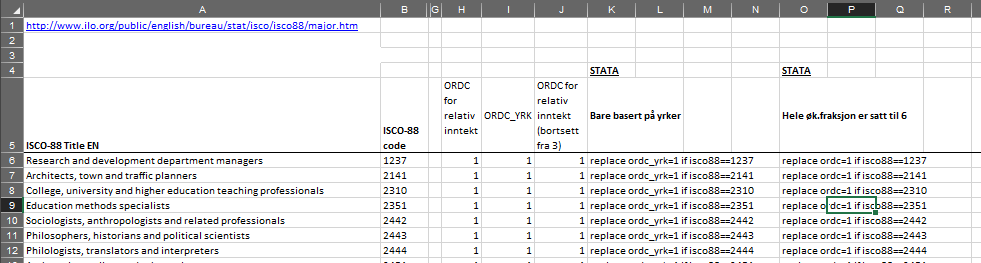
\includegraphics{./images/isco_excel.png}

Dette Excel-arket er også lagt til rette for omkoding med bruk av Stata,
men du kan se bort fra de siste kolonnene.

Filen kan leses inn med \texttt{read\_excel()}, der første linje typisk
leses inn som variabelnavn. Men i dette tilfellet skal ikke de første
linjene brukes og flere kolonner skal heller ikke brukes. Derfor ber vi
R droppe de første linjenene, endrer variabelnavn og beholder kun
isco-kodene og tilhørende ORDC-grupperingen. Variabelnavn bør ikke
inkludere mellomrom, så vi legger til et argument som endrer til gyldige
variabelnavn ved å bytte ut mellomrom med punktum. Vi også spesifiserer
\texttt{col\_types\ =\ "text"} for å unngå at tallverdier tolkes som
numeriske verdier.

\begin{Shaded}
\begin{Highlighting}[]
\FunctionTok{list.files}\NormalTok{(}\StringTok{"data/"}\NormalTok{)}
\end{Highlighting}
\end{Shaded}

\begin{verbatim}
 [1] "3_codes_isco88_ordc.xlsx" "abu89.dta"               
 [3] "CODES_isco88_ordc.xlsx"   "dat_dict.rds"            
 [5] "ESS2016.dta"              "ESS2016.rds"             
 [7] "ISCO_ORDC.do"             "norlag.rds"              
 [9] "norlag_labelled.rds"      "norlag_panel.csv"        
[11] "norlag_panel.dta"         "norlag_panel.Rdata"      
[13] "norlag_panel.rds"         "norlag_panel.sas7bdat"   
[15] "norlag_panel.sav"         "norlag_panel.xlsx"       
[17] "norlag_panel2022.dta"     "ordc.ado"                
[19] "ordc.sthlp"               "politics.csv"            
\end{verbatim}

\begin{Shaded}
\begin{Highlighting}[]
\NormalTok{isco }\OtherTok{\textless{}{-}}\NormalTok{ readxl}\SpecialCharTok{::}\FunctionTok{read\_excel}\NormalTok{(}\AttributeTok{path =} \StringTok{"data/CODES\_isco88\_ordc.xlsx"}\NormalTok{, }\AttributeTok{skip =} \DecValTok{4}\NormalTok{, }\AttributeTok{.name\_repair =} \StringTok{"universal"}\NormalTok{, }\AttributeTok{col\_types =} \StringTok{"text"}\NormalTok{) }\SpecialCharTok{\%\textgreater{}\%} 
  \FunctionTok{select}\NormalTok{(}\DecValTok{2}\NormalTok{,}\DecValTok{9}\NormalTok{) }
\FunctionTok{head}\NormalTok{(isco)}
\end{Highlighting}
\end{Shaded}

\begin{verbatim}
# A tibble: 6 x 2
  ISCO.88.code ORDC_YRK
  <chr>        <chr>   
1 1237         1       
2 2141         1       
3 2310         1       
4 2351         1       
5 2442         1       
6 2443         1       
\end{verbatim}

Now, we can merge the data with this catalogue. So that every record in
the catalogue is merged to each record with the same code. To do this,
we use \texttt{left\_join()}, and store in a new object.

\begin{Shaded}
\begin{Highlighting}[]
\NormalTok{isco }\OtherTok{\textless{}{-}}\NormalTok{ isco }\SpecialCharTok{\%\textgreater{}\%} 
  \FunctionTok{rename}\NormalTok{(}\AttributeTok{isco08 =}\NormalTok{ ISCO.}\FloatTok{88.}\NormalTok{code)}

\NormalTok{polit2 }\OtherTok{\textless{}{-}} \FunctionTok{left\_join}\NormalTok{(polit, isco, }\AttributeTok{by =} \StringTok{"isco08"}\NormalTok{)}

\FunctionTok{head}\NormalTok{(polit2)}
\end{Highlighting}
\end{Shaded}

\begin{verbatim}
  isco08 gndr polintr occupation ORDC_YRK
1   3333    1       3          3     <NA>
2   7122    1       2          7       10
3   7122    1       2          7       10
4   4221    2       4          4        8
5   4311    1       3          4     <NA>
6   6130    2       2          6       12
\end{verbatim}

What happened here is that the recoding happened almost automatically by
adding a new column with the new variable.

Now, you can make e.g.~a cross-tabulation of social class by gender.

\begin{Shaded}
\begin{Highlighting}[]
\NormalTok{polit2 }\SpecialCharTok{\%\textgreater{}\%} 
  \FunctionTok{select}\NormalTok{(ORDC\_YRK, gndr) }\SpecialCharTok{\%\textgreater{}\%} 
  \FunctionTok{tbl\_summary}\NormalTok{(}\AttributeTok{by =}\NormalTok{ gndr)}
\end{Highlighting}
\end{Shaded}

\begin{verbatim}
Table printed with `knitr::kable()`, not {gt}. Learn why at
https://www.danieldsjoberg.com/gtsummary/articles/rmarkdown.html
To suppress this message, include `message = FALSE` in code chunk header.
\end{verbatim}

\begin{longtable}[]{@{}lcc@{}}
\toprule()
\textbf{Characteristic} & \textbf{1}, N = 29,285 & \textbf{2}, N =
33,950 \\
\midrule()
\endhead
ORDC\_YRK & & \\
1 & 448 (2.4\%) & 364 (2.0\%) \\
10 & 5,887 (32\%) & 3,222 (17\%) \\
11 & 3,757 (20\%) & 5,563 (30\%) \\
12 & 1,222 (6.6\%) & 1,187 (6.4\%) \\
2 & 1,367 (7.4\%) & 1,333 (7.1\%) \\
3 & 30 (0.2\%) & 13 (\textless0.1\%) \\
4 & 561 (3.0\%) & 1,251 (6.7\%) \\
5 & 2,000 (11\%) & 2,669 (14\%) \\
6 & 1,681 (9.1\%) & 1,850 (9.9\%) \\
7 & 180 (1.0\%) & 267 (1.4\%) \\
8 & 1,129 (6.1\%) & 726 (3.9\%) \\
9 & 134 (0.7\%) & 105 (0.6\%) \\
996 & 84 (0.5\%) & 109 (0.6\%) \\
997 & 5 (\textless0.1\%) & 1 (\textless0.1\%) \\
Unknown & 10,800 & 15,290 \\
\bottomrule()
\end{longtable}

\hypertarget{noen-ganger-finnes-det-en-pakke}{%
\subsection{Noen ganger finnes det en
pakke}\label{noen-ganger-finnes-det-en-pakke}}

Siden R støtter pakker laget av brukere rundt omkring i verden, så er
det alltids en sjanse for at noen har laget noe lurt som fikser akkurat
ditt problem. Du kan altså ha flaks.

Når det gjelder omkoding av ISCO-koder til klasseskjemaer, så har noen
faktisk gjort dette. Pakken \{DIGCLASS\} koder om til flere forskjellige
klasseskjemaer ganske greit. Se gjerne nærmere på
\href{https://digclass.pages.code.europa.eu/digclass/index.html}{vignetten
til pakken}.

Denne pakken finnes imidlertid ikke på CRAN i skrivende stund. Derimot
finnes den tilgjengelig på nettet. Følgende kode installerer pakken.
Hvis du får feilmelding om at du trenger \{devtools\}, så installer
denne pakken først på vanlig måte.

\begin{Shaded}
\begin{Highlighting}[]
\NormalTok{devtools}\SpecialCharTok{::}\FunctionTok{install\_git}\NormalTok{(}\StringTok{"https://code.europa.eu/digclass/digclass.git"}\NormalTok{)}
\end{Highlighting}
\end{Shaded}

Denne pakken inneholder også funksjonen for å rydde opp i isco-kodene.
Det er noen vanlige problemer som omkodes enkelt med
\texttt{repair\_isco}. I følgende kode sjekkes isco-kodene \emph{før}
funksjonen \texttt{isco88\_to\_ordc} brukes til selve omkodingen. Den
har en versjon som gir tallkode og en som gir tekstverdier, som er
kjekt, så da kjøres begge to.

Denne funksjonen spytter også ut mange beskjeder i output som vi strengt
tatt ikke trenger. Den melder fra om alle verdier som ikke inngår i
klasseskjemaet og som derfor settes til NA. Det er fint, men tar i dette
tilfellet ganske mye plass. Vet å bruke funksjonen
\texttt{suppressMessages(\{...\})} og parenteser rundt hele koden
slipper vi dette. Normalt skal du ikke bruke denne funksjonen da du
vanligvis vil ha slike beskjeder. Her tar det bare litt mye plass.

\begin{Shaded}
\begin{Highlighting}[]
\FunctionTok{library}\NormalTok{(DIGCLASS)}

\FunctionTok{suppressMessages}\NormalTok{(\{}
\NormalTok{polit3 }\OtherTok{\textless{}{-}}\NormalTok{ polit }\SpecialCharTok{\%\textgreater{}\%} 
  \FunctionTok{mutate}\NormalTok{(}\AttributeTok{isco08 =} \FunctionTok{repair\_isco}\NormalTok{(.}\SpecialCharTok{$}\NormalTok{isco08), }
         \AttributeTok{orcd =} \FunctionTok{isco88\_to\_ordc}\NormalTok{(isco08, }\AttributeTok{label =} \ConstantTok{FALSE}\NormalTok{), }
         \AttributeTok{orcd\_lab =} \FunctionTok{isco88\_to\_ordc}\NormalTok{(isco08, }\AttributeTok{label =} \ConstantTok{TRUE}\NormalTok{))}
\NormalTok{\})}

\FunctionTok{head}\NormalTok{(polit3)}
\end{Highlighting}
\end{Shaded}

\begin{verbatim}
  isco08 gndr polintr occupation orcd                     orcd_lab
1   3333    1       3          3 <NA>                         <NA>
2   7122    1       2          7   10        Skilled working class
3   4221    2       4          4    8 Lower-middle class: balanced
4   4311    1       3          4 <NA>                         <NA>
5   6130    2       2          6   12     Primary-sector employees
6   7212    1       2          7   10        Skilled working class
\end{verbatim}

Da kan vi lage tabellen omigjen bare for å sjekke at vi får samme svar.

\begin{Shaded}
\begin{Highlighting}[]
\NormalTok{polit3 }\SpecialCharTok{\%\textgreater{}\%} 
  \FunctionTok{select}\NormalTok{(orcd, gndr) }\SpecialCharTok{\%\textgreater{}\%} 
  \FunctionTok{tbl\_summary}\NormalTok{(}\AttributeTok{by =}\NormalTok{ gndr)}
\end{Highlighting}
\end{Shaded}

\begin{verbatim}
Table printed with `knitr::kable()`, not {gt}. Learn why at
https://www.danieldsjoberg.com/gtsummary/articles/rmarkdown.html
To suppress this message, include `message = FALSE` in code chunk header.
\end{verbatim}

\begin{longtable}[]{@{}lcc@{}}
\toprule()
\textbf{Characteristic} & \textbf{1}, N = 23,020 & \textbf{2}, N =
26,499 \\
\midrule()
\endhead
orcd & & \\
1 & 190 (1.6\%) & 182 (1.6\%) \\
10 & 4,188 (36\%) & 1,890 (17\%) \\
11 & 2,075 (18\%) & 2,564 (23\%) \\
12 & 723 (6.2\%) & 669 (6.0\%) \\
13 & 80 (0.7\%) & 101 (0.9\%) \\
2 & 1,014 (8.7\%) & 838 (7.5\%) \\
3 & 10 (\textless0.1\%) & 2 (\textless0.1\%) \\
4 & 316 (2.7\%) & 604 (5.4\%) \\
5 & 947 (8.1\%) & 1,062 (9.5\%) \\
6 & 572 (4.9\%) & 639 (5.7\%) \\
7 & 226 (1.9\%) & 422 (3.8\%) \\
8 & 1,137 (9.8\%) & 1,882 (17\%) \\
9 & 167 (1.4\%) & 333 (3.0\%) \\
Unknown & 11,375 & 15,311 \\
\bottomrule()
\end{longtable}

\begin{verbatim}



## Gjøre samme ting med mange variable med `across()`






::: {.quarto-book-part}


`<!-- quarto-file-metadata: eyJyZXNvdXJjZURpciI6Ii4ifQ== -->`{=html}

```{=html}
<!-- quarto-file-metadata: eyJyZXNvdXJjZURpciI6Ii4iLCJib29rSXRlbVR5cGUiOiJhcHBlbmRpeCIsImJvb2tJdGVtTnVtYmVyIjpudWxsLCJib29rSXRlbURlcHRoIjowfQ== -->
\end{verbatim}

\hypertarget{appendices}{%
\chapter*{Appendices}\label{appendices}}
\addcontentsline{toc}{chapter}{Appendices}

\markboth{Appendices}{Appendices}

:::

\hypertarget{import-av-data-fra-sikt---huxe5ndtering-av-formater-med-metadata}{%
\chapter{Import av data fra Sikt - håndtering av formater med
metadata}\label{import-av-data-fra-sikt---huxe5ndtering-av-formater-med-metadata}}

For de som vil ha en litt mer utfordring kan man lese inn filen i
Stata-format. Dette er slik det blir levert fra Sikt\footnote{Det kan
  sies mye om å levere ut data på denne måten, men det vil ikke ta seg
  ut å gjøre det i undervisningsmateriale.}

Stata-formatet dta har to utfordringer når vi importerer til R. Det er
tilsvarende problemstilling hvis man importerer fra SPSS eller SAS. For
det første er det noen ganger gitt en egen kode for manglende verdi,
såkalt ``missing''. For det andre lagres informasjonen på en annen måte
enn i R. I Stata er ofte kategoriske variable lagret som en numerisk
variabel med en tilhørende ``label''. Når man leser inn dta-fil til R
vil disse variablene være av typen ``labelled''. I R er det langt bedre
å gjøre de om til factor-variable, men det er litt styr å kode om hvis
det er veldig mange variable i datasettet - slik det ofte er i
surveydata.

Vi presenterer en samlet løsning først, så tar vi hver del for seg
etterpå for å forklare. Nedenforstående kode gjør omtrent følgende:

\begin{itemize}
\tightlist
\item
  Leser inn en dta-fil
\item
  Omkoder alle spesifiserte missing-verdier til NA. Dette gjøres for
  \emph{alle} variable i hele datasettet (altså hundrevis av variable)
\item
  Fjerner alle labler som ikke er i bruk (altså: labler for ulike
  missing-verdier)
\item
  Gjør om alle variable av typen ``labelled'' til factor-variable
\end{itemize}

\hypertarget{huxe5ndtering-av-user-nas}{%
\section{Håndtering av user-NAs}\label{huxe5ndtering-av-user-nas}}

For disse dataene vil det være ulike sett av missing-verdier for de
ulike variablene. Dette kan helt fint håndteres manuelt variabel for
variabel. Men for å ha ordentlig kontroll på at det blir riktig bør det
automatiseres. Logikken i denne delen går et stykke utover hva vi
forventer at den jevne sosiologistudent skal lære.

En første sted er å lese inn dokumentasjonsrapporten fra en html-fil
slik den leveres fra Sikt og gjør det om til et håndterbart
oppslags-datasett. Dette er beskrevet i eget appendix. Det følgende tar
utgangspunkt i at en slik oppslagsfil finnes.

Det er noen verdier som i dokumentasjonen er spesifisert som spesielle
typer missing. Disse skal vi kode om til NA. Disse verdiene har labler
som starter med ``filter:'' eller ``vil ikke svare'' etc. Disse danner
basis for omkoding til \texttt{NA}. Dette er ikke en komplett liste over
koder som innebærer at det egentlig mangler informasjon. (Dvs. fordi
koden indikerer grunner til at det mangler informasjon). Etter denne
oppryddingen kan det altså fremdeles hende at det dukker opp noe slikt,
så vær påpasselig med å sjekke variabelens fordeling før du analyserer
med regresjonsmodeller.

Funksjonen nedenfor skal brukes innenfor et steg der man går gjennom
alle variablene en om gangen. For hver variabel slås det opp de aktuelle
missing-verdiene som gjelder for denne og bruker \texttt{replace} til å
omkode til \texttt{NA} for disse verdiene. Når denne funksjonen kalles
for hver variabel senere, så brukes det altså ulike definisjoner av
missing-verdier for hver variabel.\^{}(Basert på kode fra
https://tim-tiefenbach.de/post/2023-recode-columns/ )

\begin{Shaded}
\begin{Highlighting}[]
\CommentTok{\# leser inn kodeliste/dokumentasjon}
\NormalTok{dat\_dict }\OtherTok{\textless{}{-}} \FunctionTok{readRDS}\NormalTok{(}\StringTok{"data/dat\_dict.rds"}\NormalTok{)}

\CommentTok{\# velger kun missing{-}lablene}
\NormalTok{dat\_dict\_na }\OtherTok{\textless{}{-}}\NormalTok{ dat\_dict }\SpecialCharTok{\%\textgreater{}\%} 
  \FunctionTok{filter}\NormalTok{(  }\FunctionTok{str\_sub}\NormalTok{(}\FunctionTok{tolower}\NormalTok{(label), }\DecValTok{1}\NormalTok{, }\DecValTok{7}\NormalTok{) }\SpecialCharTok{==} \StringTok{"filter:"} \SpecialCharTok{|} 
           \FunctionTok{str\_sub}\NormalTok{(}\FunctionTok{tolower}\NormalTok{(label), }\DecValTok{1}\NormalTok{, }\DecValTok{10}\NormalTok{) }\SpecialCharTok{==} \StringTok{"filterfeil"} \SpecialCharTok{|}
           \FunctionTok{str\_sub}\NormalTok{(}\FunctionTok{tolower}\NormalTok{(label), }\DecValTok{1}\NormalTok{, }\DecValTok{12}\NormalTok{) }\SpecialCharTok{==} \StringTok{"ikke besvart"} \SpecialCharTok{|}
           \FunctionTok{str\_sub}\NormalTok{(}\FunctionTok{tolower}\NormalTok{(label), }\DecValTok{1}\NormalTok{, }\DecValTok{9}\NormalTok{) }\SpecialCharTok{\%in\%} \FunctionTok{c}\NormalTok{(}\StringTok{"filter t2"}\NormalTok{, }\StringTok{"filter t1"}\NormalTok{, }\StringTok{"filter t3"}\NormalTok{) }\SpecialCharTok{|}
           \FunctionTok{tolower}\NormalTok{(label) }\SpecialCharTok{\%in\%} \FunctionTok{c}\NormalTok{(}\StringTok{"vil ikke svare"}\NormalTok{,}
                                 \StringTok{"deltok ikke i runden"}\NormalTok{,}
                                 \StringTok{"mangler data"}\NormalTok{, }\StringTok{"manglende data"}\NormalTok{, }
                                 \StringTok{"mangler verdi"}\NormalTok{, }\StringTok{"ubesvart spørsmål"}\NormalTok{, }
                                 \StringTok{"ugyldig verdi"}\NormalTok{, }\StringTok{"oppgitt verdi ikke et årstall"}\NormalTok{,}
                                 \StringTok{"filter {-}"}\NormalTok{,}
                                 \StringTok{"ikke svart post/web skjema"}\NormalTok{)) }

\CommentTok{\# Funksjon for å recode som har gitte user{-}NA.}
\CommentTok{\# (Må brukes innenfor \textasciigrave{}across()\textasciigrave{} nedenfor)}
\NormalTok{recode\_col\_na }\OtherTok{\textless{}{-}} \ControlFlowTok{function}\NormalTok{(x, dict) \{}
\NormalTok{  recode\_vec }\OtherTok{\textless{}{-}}\NormalTok{ dict }\SpecialCharTok{\%\textgreater{}\%}
    \FunctionTok{filter}\NormalTok{(col\_nm }\SpecialCharTok{==} \FunctionTok{cur\_column}\NormalTok{()) }\SpecialCharTok{\%\textgreater{}\%}
    \FunctionTok{mutate}\NormalTok{(}\AttributeTok{value =} \FunctionTok{as.numeric}\NormalTok{(value)) }\SpecialCharTok{\%\textgreater{}\%} 
    \FunctionTok{pull}\NormalTok{(value)}
  \FunctionTok{replace}\NormalTok{(x, x }\SpecialCharTok{\%in\%}\NormalTok{ recode\_vec, }\ConstantTok{NA}\NormalTok{)}
\NormalTok{\}}
\end{Highlighting}
\end{Shaded}

\hypertarget{innlesning-av-data-2}{%
\section{innlesning av data}\label{innlesning-av-data-2}}

\begin{Shaded}
\begin{Highlighting}[]
\FunctionTok{library}\NormalTok{(tidyverse)}
\FunctionTok{library}\NormalTok{(haven)}
\FunctionTok{library}\NormalTok{(labelled)}


\CommentTok{\# data}
\NormalTok{faste }\OtherTok{\textless{}{-}} \FunctionTok{read\_stata}\NormalTok{( }\FunctionTok{paste0}\NormalTok{(infilbane, }\StringTok{"NorLAG{-}lengde{-}faste.dta"}\NormalTok{), }\AttributeTok{encoding =} \StringTok{"utf{-}8"}\NormalTok{)}

\NormalTok{lang }\OtherTok{\textless{}{-}} \FunctionTok{read\_stata}\NormalTok{( }\FunctionTok{paste0}\NormalTok{(infilbane, }\StringTok{"NorLAG{-}lengde{-}intervju.dta"}\NormalTok{), }\AttributeTok{encoding =} \StringTok{"utf{-}8"}\NormalTok{)}



\NormalTok{norlag\_lbl }\OtherTok{\textless{}{-}} \FunctionTok{merge}\NormalTok{(faste, lang, }\AttributeTok{by =} \FunctionTok{c}\NormalTok{(}\StringTok{"ref\_nr"}\NormalTok{), }\AttributeTok{all.y =} \ConstantTok{TRUE}\NormalTok{) }\SpecialCharTok{\%\textgreater{}\%} 
  \FunctionTok{filter}\NormalTok{(iodeltakelse }\SpecialCharTok{==} \DecValTok{1} \SpecialCharTok{|}  
\NormalTok{           iodeltakelse }\SpecialCharTok{==} \DecValTok{2} \SpecialCharTok{\&}\NormalTok{ round }\SpecialCharTok{\%in\%} \FunctionTok{c}\NormalTok{(}\DecValTok{1}\NormalTok{, }\DecValTok{3}\NormalTok{) }\SpecialCharTok{|} 
\NormalTok{           iodeltakelse }\SpecialCharTok{==} \DecValTok{3} \SpecialCharTok{\&}\NormalTok{ round }\SpecialCharTok{\%in\%} \FunctionTok{c}\NormalTok{(}\DecValTok{2}\NormalTok{, }\DecValTok{3}\NormalTok{) }\SpecialCharTok{|}
\NormalTok{           iodeltakelse }\SpecialCharTok{==} \DecValTok{4} \SpecialCharTok{\&}\NormalTok{ round }\SpecialCharTok{\%in\%} \FunctionTok{c}\NormalTok{(}\DecValTok{1}\NormalTok{) }\SpecialCharTok{|}
\NormalTok{           iodeltakelse }\SpecialCharTok{==} \DecValTok{5} \SpecialCharTok{\&}\NormalTok{ round }\SpecialCharTok{\%in\%} \FunctionTok{c}\NormalTok{(}\DecValTok{1}\NormalTok{, }\DecValTok{2}\NormalTok{) }\SpecialCharTok{|}
\NormalTok{           iodeltakelse }\SpecialCharTok{==} \DecValTok{6} \SpecialCharTok{\&}\NormalTok{ round }\SpecialCharTok{\%in\%} \FunctionTok{c}\NormalTok{(}\DecValTok{2}\NormalTok{)}
\NormalTok{  ) }



\CommentTok{\# vektorer av variable som skal omkodes}
\NormalTok{cols\_vec\_all }\OtherTok{\textless{}{-}} \FunctionTok{unique}\NormalTok{(dat\_dict}\SpecialCharTok{$}\NormalTok{col\_nm)}
\NormalTok{vars }\OtherTok{\textless{}{-}} \FunctionTok{unique}\NormalTok{(}\FunctionTok{names}\NormalTok{(norlag\_lbl))}
\NormalTok{cols\_vec }\OtherTok{\textless{}{-}}\NormalTok{ cols\_vec\_all[cols\_vec\_all }\SpecialCharTok{\%in\%}\NormalTok{ vars]}
\NormalTok{cols\_vec\_na }\OtherTok{\textless{}{-}}\NormalTok{ cols\_vec[(cols\_vec }\SpecialCharTok{\%in\%} \FunctionTok{unique}\NormalTok{(dat\_dict\_na}\SpecialCharTok{$}\NormalTok{col\_nm))]}

\NormalTok{norlag }\OtherTok{\textless{}{-}}\NormalTok{ norlag\_lbl }\SpecialCharTok{\%\textgreater{}\%} 
  \FunctionTok{mutate}\NormalTok{(}\FunctionTok{across}\NormalTok{(}\FunctionTok{all\_of}\NormalTok{(cols\_vec\_na), }
\NormalTok{              \textbackslash{}(x,dic) }\FunctionTok{recode\_col\_na}\NormalTok{(x, .env}\SpecialCharTok{$}\NormalTok{dat\_dict\_na))) }\SpecialCharTok{\%\textgreater{}\%} 
  \FunctionTok{mutate}\NormalTok{(}\FunctionTok{across}\NormalTok{(}\FunctionTok{where}\NormalTok{(is.labelled), }\SpecialCharTok{\textasciitilde{}}\FunctionTok{as\_factor}\NormalTok{(.))) }\SpecialCharTok{\%\textgreater{}\%} 
  \FunctionTok{mutate}\NormalTok{(}\FunctionTok{across}\NormalTok{(}\FunctionTok{where}\NormalTok{(is.factor), }\SpecialCharTok{\textasciitilde{}}\FunctionTok{fct\_drop}\NormalTok{(.)))}
\end{Highlighting}
\end{Shaded}

I tilegg skal vi lage en variabel for det vi kan kalle hovedaktivitet
som sysselsettingsstatus. Det er om man er yrkesaktiv, arbeidsledig,
student eller annet. I hver runde av NorLAG ble svarkategoriene utformet
litt forskjellig, så derfor er svarene fordelt over tre variable.
Nedenfor samles disse sammen og kodes om basert på tekststrenger.

\begin{Shaded}
\begin{Highlighting}[]
\DocumentationTok{\#\# Omkoder hovedaktivitet }
\NormalTok{fs }\OtherTok{\textless{}{-}} \FunctionTok{lvls\_union}\NormalTok{( }\FunctionTok{list}\NormalTok{(norlag}\SpecialCharTok{$}\NormalTok{wr001, norlag}\SpecialCharTok{$}\NormalTok{wr002, norlag}\SpecialCharTok{$}\NormalTok{wr003c)) }\SpecialCharTok{\%\textgreater{}\%} \FunctionTok{tolower}\NormalTok{() }\SpecialCharTok{\%\textgreater{}\%} \FunctionTok{unique}\NormalTok{()}

\NormalTok{norlag }\OtherTok{\textless{}{-}}\NormalTok{ norlag }\SpecialCharTok{\%\textgreater{}\%} 
  \FunctionTok{mutate}\NormalTok{(}\FunctionTok{across}\NormalTok{(wr001}\SpecialCharTok{:}\NormalTok{wr003c, }\SpecialCharTok{\textasciitilde{}}\FunctionTok{factor}\NormalTok{(}\FunctionTok{tolower}\NormalTok{(.), }\AttributeTok{levels=}\NormalTok{fs))) }\SpecialCharTok{\%\textgreater{}\%} 
  \FunctionTok{mutate}\NormalTok{(}\AttributeTok{hovedaktivitet =} \FunctionTok{case\_when}\NormalTok{(round }\SpecialCharTok{==} \DecValTok{1} \SpecialCharTok{\textasciitilde{}}\NormalTok{ wr001, }
\NormalTok{                                    round }\SpecialCharTok{==} \DecValTok{2} \SpecialCharTok{\textasciitilde{}}\NormalTok{ wr002, }
\NormalTok{                                    round }\SpecialCharTok{==} \DecValTok{3} \SpecialCharTok{\textasciitilde{}}\NormalTok{ wr003c) ) }\SpecialCharTok{\%\textgreater{}\%} 
  \FunctionTok{mutate}\NormalTok{(}\AttributeTok{hovedaktivitet2 =} \FunctionTok{case\_when}\NormalTok{( }\FunctionTok{str\_sub}\NormalTok{(hovedaktivitet, }\DecValTok{1}\NormalTok{, }\DecValTok{5}\NormalTok{) }\SpecialCharTok{==} \StringTok{"yrkes"} \SpecialCharTok{\textasciitilde{}} \StringTok{"Yrkesaktiv"}\NormalTok{, }
                                      \FunctionTok{str\_detect}\NormalTok{(hovedaktivitet, }\StringTok{"arbeidsledig"}\NormalTok{) }\SpecialCharTok{\textasciitilde{}} \StringTok{"Trygdet/arbeidsledig/stud/annet"}\NormalTok{, }
                                      \FunctionTok{str\_detect}\NormalTok{(hovedaktivitet, }\StringTok{"student"}\NormalTok{) }\SpecialCharTok{\textasciitilde{}} \StringTok{"Trygdet/arbeidsledig/stud/annet"}\NormalTok{, }
                                      \FunctionTok{str\_detect}\NormalTok{(hovedaktivitet, }\StringTok{"trygd"}\NormalTok{) }\SpecialCharTok{\textasciitilde{}} \StringTok{"Trygdet/arbeidsledig/stud/annet"}\NormalTok{, }
                                      \FunctionTok{str\_detect}\NormalTok{(hovedaktivitet, }\StringTok{"annet"}\NormalTok{) }\SpecialCharTok{\textasciitilde{}} \StringTok{"Trygdet/arbeidsledig/stud/annet"}\NormalTok{, }
                                      \FunctionTok{str\_sub}\NormalTok{(hovedaktivitet,}\DecValTok{1}\NormalTok{,}\DecValTok{6}\NormalTok{)   }\SpecialCharTok{==} \StringTok{"hjemme"} \SpecialCharTok{\textasciitilde{}} \StringTok{"hjemmeværende/husmor"}\NormalTok{, }
                                      \FunctionTok{str\_detect}\NormalTok{(hovedaktivitet, }\StringTok{"pensjonist"}\NormalTok{) }\SpecialCharTok{\textasciitilde{}} \StringTok{"pensjonist"}\NormalTok{, }
                                      \FunctionTok{is.na}\NormalTok{(hovedaktivitet) }\SpecialCharTok{\textasciitilde{}} \StringTok{"Trygdet/arbeidsledig/stud/annet"}\NormalTok{) }\SpecialCharTok{\%\textgreater{}\%} \FunctionTok{as\_factor}\NormalTok{())}
\end{Highlighting}
\end{Shaded}

Og dermed har vi et datasett i et svært så ryddig R-format.

\hypertarget{hvordan-fungerer-koden-ovenfor-en-intro-til-mer-avansert-databehandling}{%
\section{Hvordan fungerer koden ovenfor?? En intro til mer avansert
databehandling}\label{hvordan-fungerer-koden-ovenfor-en-intro-til-mer-avansert-databehandling}}

\hypertarget{sjekk-datastruktur-og-bruk-av-filter}{%
\subsection{\texorpdfstring{Sjekk datastruktur og bruk av
\texttt{filter}}{Sjekk datastruktur og bruk av filter}}\label{sjekk-datastruktur-og-bruk-av-filter}}

\hypertarget{omkode-bruker-spesifiserte-missing-verdier-til-na}{%
\subsection{\texorpdfstring{Omkode bruker-spesifiserte missing-verdier
til
\texttt{NA}}{Omkode bruker-spesifiserte missing-verdier til NA}}\label{omkode-bruker-spesifiserte-missing-verdier-til-na}}

\hypertarget{kode-om-puxe5-tvers-av-mange-variable-med-across}{%
\subsection{\texorpdfstring{Kode om på tvers av mange variable med
\texttt{across}}{Kode om på tvers av mange variable med across}}\label{kode-om-puxe5-tvers-av-mange-variable-med-across}}

\hypertarget{fjerne-nivuxe5er-som-ikke-brukes-drop_unused_value_labels}{%
\subsection{\texorpdfstring{Fjerne nivåer som ikke brukes:
\texttt{drop\_unused\_value\_labels}}{Fjerne nivåer som ikke brukes: drop\_unused\_value\_labels}}\label{fjerne-nivuxe5er-som-ikke-brukes-drop_unused_value_labels}}

\hypertarget{gjuxf8r-om-til-factor-med-unlabelled}{%
\subsection{\texorpdfstring{Gjør om til factor med
\texttt{unlabelled}}{Gjør om til factor med unlabelled}}\label{gjuxf8r-om-til-factor-med-unlabelled}}

\hypertarget{for-spesielt-interesserte-jobbe-med-labelled-data}{%
\section{For spesielt interesserte: jobbe med
labelled-data}\label{for-spesielt-interesserte-jobbe-med-labelled-data}}

\hypertarget{lage-dictionary-fil}{%
\chapter{Lage dictionary-fil}\label{lage-dictionary-fil}}

Dokumentasjonen som følger med NorLAG og andre datasett fra Sikt er en
html-fil (dvs. web-side) med en oversikt over alle variable og hvordan
de er kodet. Dette er fint for manuelt oppslag, men er ikke ideelt til
bruk for maskinell behandling.

Det vi ideelt skulle hatt er et samlet datasett der kodeskjemaet er
knyttet til variabelnavnene. Dette kalles noen ganger en ``dictionary''
fil. All informasjonen vi trenger for å lage en slik ligger i html-filen
man får sammen med datasettet fra Sikt, bare på en knotete form. Det
skal vi fikse.

Nedenfor skal vi vise hvordan vi gjør følgende:

\begin{itemize}
\tightlist
\item
  Leser inn en fullstendig html-fil, inkludert alle html-kodene
\item
  Identifiserer den delen av html-filen som inneholder kodeskjema og
  begrenser filen til disse
\item
  Plukker ut alle tabeller og gjør dem om til data.frame-struktur i R
\item
  Rensker opp i filen til å bare beholde de relevante radene
\end{itemize}

Dette er egentlig en svært enkel introduksjon til webscraping for et
spesfikt formål. Vi skal bruke pakken \texttt{rvest} som er laget
nettopp for webscraping.

\begin{Shaded}
\begin{Highlighting}[]
\FunctionTok{library}\NormalTok{(rvest)       }\CommentTok{\# scrape html{-}sider}
\FunctionTok{library}\NormalTok{(tidyverse)   }\CommentTok{\# generell databehandling}
\end{Highlighting}
\end{Shaded}

\hypertarget{lese-inn-html-dokumentasjonen}{%
\section{Lese inn
html-dokumentasjonen}\label{lese-inn-html-dokumentasjonen}}

Første sted er å lese inn html-filen. Funksjonen \texttt{read\_html()}
gjør dette. For å skjønne litt mer av hvordan dette ser ut kan du åpne
den opprinnelige html-filen i ren tekst, f.eks. med bruk av Notepad. Det
er dette som leses inn. Jeg legger det i et nytt objekt som jeg har kalt
\texttt{cb} (forkortelse for codebook).

\begin{Shaded}
\begin{Highlighting}[]
\CommentTok{\#library(XML)}

\CommentTok{\# read html file}
\NormalTok{u }\OtherTok{\textless{}{-}} \StringTok{"C:/Users/torbskar/OneDrive {-} Universitetet i Oslo/Dokumenter/Undervisning/SOS4020\_forkurs/data2023/data\_tilDeling/Kodebok.html"}

\NormalTok{cb }\OtherTok{\textless{}{-}} \FunctionTok{read\_html}\NormalTok{(u)}
\end{Highlighting}
\end{Shaded}

For NorLAG er dokumentasjonsdokumentet inndelt i flere deler, og det er
bare den siste delen som inneholder kodeskjemaene. Det er denne siste
delen vi trenger, så første utfordring er å plukke ut denne delen.

En html-fil er strukturert innenfor ``noder'' som har en start og en
slutt. Et avsnitt starter med en kode
\texttt{\textless{}a\textgreater{}} og avsluttes med
\texttt{\textless{}/a\textgreater{}}. Tilsvarende koder finnes for
tabeller og andre elementer. Disse delene har er oftest gitt et navn som
man kan identififiseres og brukes til lage lenker til spesifikke deler
av siden (jf. innholdsfortegnelsen). Vi bruker denne til å filtrere
filen.

I akkurat denne filen trenger vi informasjonen som ligger etter
overskriften ``Variables Description''. For å finne navnet på dette
avsnittet kan man undersøke lenken i innholdsfortegnelsen der det
fremkommer som \texttt{\#variables}. Eller man kan åpne html-filen i et
tekstdokument og søke opp tittelen, så finner man koden
\texttt{name=\textquotesingle{}variables} innenfor det avsnittet.

Vi bruker \texttt{html\_nodes} til å trekke ut bare dette avsnittet som
følger.

\begin{Shaded}
\begin{Highlighting}[]
\CommentTok{\# Find the specific heading}
\NormalTok{variables }\OtherTok{\textless{}{-}}\NormalTok{ cb }\SpecialCharTok{\%\textgreater{}\%} 
  \FunctionTok{html\_nodes}\NormalTok{(}\StringTok{"a[name=\textquotesingle{}variables\textquotesingle{}]"}\NormalTok{)}
\end{Highlighting}
\end{Shaded}

I denne dokumentasjonen er hver variabel lagret i en egen tabell. I
html-kode angis begynnelsen av en tabell med
\texttt{\textless{}table\textgreater{}} og denne brukes til å trekke ut
bare tabellene.

\begin{Shaded}
\begin{Highlighting}[]
\NormalTok{tables }\OtherTok{\textless{}{-}}\NormalTok{ variables }\SpecialCharTok{\%\textgreater{}\%} 
    \CommentTok{\#html\_node(xpath = "//a[@name=\textquotesingle{}variables\textquotesingle{}]") \%\textgreater{}\% }
    \FunctionTok{html\_nodes}\NormalTok{(}\AttributeTok{xpath =} \StringTok{"./following::table"}\NormalTok{)}
\end{Highlighting}
\end{Shaded}

Så kan vi bruke funksjonen \texttt{html\_table} til å trekke ut hver
enkelt tabell i en struktur som er lettere å jobbe med, nemlig en
``data.frame'', altså en rektangulær struktur med rader og kolonner slik
datasett vanligvis ser ut. Hver tabell blir et eget data.frame-objekt,
og når man legger dette i et nytt objekt blir det av typen ``list''. En
``list'' er en samling objekter som har hver sin plass i det samme
objektet. (Du kan tenke på det som en eske med flere mindre ekster
oppi). Vi kommer tilbake til hvordan de slås sammen.

\begin{Shaded}
\begin{Highlighting}[]
\NormalTok{table\_data }\OtherTok{\textless{}{-}} \FunctionTok{html\_table}\NormalTok{(tables)}
\end{Highlighting}
\end{Shaded}

\hypertarget{legge-det-hele-i-en-funksjon}{%
\subsection{Legge det hele i en
funksjon}\label{legge-det-hele-i-en-funksjon}}

\begin{Shaded}
\begin{Highlighting}[]
\CommentTok{\# Check if the heading exists}
\ControlFlowTok{if}\NormalTok{ (}\FunctionTok{length}\NormalTok{(variables) }\SpecialCharTok{\textgreater{}} \DecValTok{0}\NormalTok{) \{}
  \CommentTok{\# Find the tables after the heading}
\NormalTok{  tables }\OtherTok{\textless{}{-}}\NormalTok{ variables }\SpecialCharTok{\%\textgreater{}\%} 
    \FunctionTok{html\_node}\NormalTok{(}\AttributeTok{xpath =} \StringTok{"//a[@name=\textquotesingle{}variables\textquotesingle{}]"}\NormalTok{) }\SpecialCharTok{\%\textgreater{}\%} 
    \FunctionTok{html\_nodes}\NormalTok{(}\AttributeTok{xpath =} \StringTok{"./following::table"}\NormalTok{)}
  
  \CommentTok{\# Extract the table data}
\NormalTok{  table\_data }\OtherTok{\textless{}{-}} \FunctionTok{html\_table}\NormalTok{(tables)}
\NormalTok{  \} }\ControlFlowTok{else}\NormalTok{ \{}
  \FunctionTok{cat}\NormalTok{(}\StringTok{"The specified heading was not found."}\NormalTok{)}
\NormalTok{\}}


\NormalTok{tbslist }\OtherTok{\textless{}{-}} \FunctionTok{list}\NormalTok{()}
\ControlFlowTok{for}\NormalTok{(i }\ControlFlowTok{in} \DecValTok{1}\SpecialCharTok{:}\FunctionTok{length}\NormalTok{(table\_data))\{ }
  \ControlFlowTok{if}\NormalTok{(}\StringTok{"X2"} \SpecialCharTok{\%in\%} \FunctionTok{names}\NormalTok{(table\_data[[i]]) }\SpecialCharTok{\&} 
     \StringTok{"X3"} \SpecialCharTok{\%in\%} \FunctionTok{names}\NormalTok{(table\_data[[i]]) }\SpecialCharTok{\&} 
     \SpecialCharTok{!}\NormalTok{(}\StringTok{"X4"} \SpecialCharTok{\%in\%} \FunctionTok{names}\NormalTok{(table\_data[[i]])) )\{}
    
\NormalTok{    tbslist[[i]] }\OtherTok{\textless{}{-}}\NormalTok{ table\_data[[i]] }\SpecialCharTok{\%\textgreater{}\%} 
      \FunctionTok{mutate}\NormalTok{(}\AttributeTok{col\_nm =} \FunctionTok{strsplit}\NormalTok{(}\FunctionTok{as.character}\NormalTok{(.[}\DecValTok{1}\NormalTok{,}\DecValTok{1}\NormalTok{]), }\AttributeTok{split =} \StringTok{":"}\NormalTok{)[[}\DecValTok{1}\NormalTok{]][}\DecValTok{1}\NormalTok{],}
             \AttributeTok{spm =} \FunctionTok{strsplit}\NormalTok{(}\FunctionTok{as.character}\NormalTok{(.[}\DecValTok{1}\NormalTok{,}\DecValTok{1}\NormalTok{]), }\AttributeTok{split =} \StringTok{":"}\NormalTok{)[[}\DecValTok{1}\NormalTok{]][}\DecValTok{2}\NormalTok{]) }\SpecialCharTok{\%\textgreater{}\%} 
      \FunctionTok{rename}\NormalTok{( }\AttributeTok{value =}\NormalTok{ X2, }
              \AttributeTok{label =}\NormalTok{ X3) }\SpecialCharTok{\%\textgreater{}\%}
      \FunctionTok{filter}\NormalTok{( }\FunctionTok{str\_detect}\NormalTok{(X1, }\StringTok{"Values and categories"}\NormalTok{)) }\SpecialCharTok{\%\textgreater{}\%} 
      \FunctionTok{filter}\NormalTok{( }\SpecialCharTok{!}\FunctionTok{is.na}\NormalTok{(value)) }\SpecialCharTok{\%\textgreater{}\%} 
      \FunctionTok{select}\NormalTok{(}\SpecialCharTok{{-}}\NormalTok{X1)}
\NormalTok{  \}}
  \ControlFlowTok{else}\NormalTok{\{}
    \ControlFlowTok{if}\NormalTok{(i}\SpecialCharTok{==}\DecValTok{1}\NormalTok{)\{}
\NormalTok{      teller }\OtherTok{\textless{}{-}} \DecValTok{0}
\NormalTok{      \}}
\NormalTok{    teller }\OtherTok{\textless{}{-}}\NormalTok{ teller }\SpecialCharTok{+} \DecValTok{1} 
\NormalTok{  \}}
  \ControlFlowTok{if}\NormalTok{(i }\SpecialCharTok{==} \FunctionTok{length}\NormalTok{(table\_data))\{}
    \FunctionTok{print}\NormalTok{(}\FunctionTok{paste}\NormalTok{(}\StringTok{"Antall variable som ikke har omkodinger: "}\NormalTok{, teller)) }
\NormalTok{  \}}
\NormalTok{\}}
\end{Highlighting}
\end{Shaded}

\begin{verbatim}
[1] "Antall variable som ikke har omkodinger:  1"
\end{verbatim}

\begin{Shaded}
\begin{Highlighting}[]
\NormalTok{dat\_dict }\OtherTok{\textless{}{-}} \FunctionTok{bind\_rows}\NormalTok{(tbslist) }\SpecialCharTok{\%\textgreater{}\%} 
  \FunctionTok{select}\NormalTok{(col\_nm, value, label, spm)}
\end{Highlighting}
\end{Shaded}

\begin{Shaded}
\begin{Highlighting}[]
\FunctionTok{saveRDS}\NormalTok{(dat\_dict, }\StringTok{"data/dat\_dict.rds"}\NormalTok{)}
\end{Highlighting}
\end{Shaded}




\end{document}
